% REMEMBER: You must not plagiarise anything in your report. Be extremely careful.

\documentclass{l4proj}

    
%
% put any additional packages here
%
\usepackage{graphicx}
\usepackage{multirow}
\begin{document}

%==============================================================================
%% METADATA
\title{The Sensitivity of Facial Analysis Algorithms to Race and Gender}
\author{Mohammed Zeerak}
\date{April 8, 2021}

\maketitle

%==============================================================================
%% ABSTRACT
\begin{abstract}
    % Every abstract follows a similar pattern. Motivate; set aims; describe work; explain results.
    % \vskip 0.5em
    % ``XYZ is bad. This project investigated ABC to determine if it was better. 
    % ABC used XXX and YYY to implement ZZZ. This is particularly interesting as XXX and YYY have
    % never been used together. It was found that  
    % ABC was 20\% better than XYZ, though it caused rabies in half of subjects.''
    
    Facial detection bias between races and gender is a serious concern within the field of computer vision. This technology is seeing practical use in the real world, therefore any bias present could incur detrimental consequences for the targeted group. This project investigated a range of facial detection algorithms to understand if, and why there existed a bias towards race and gender. The Viola-Jones, HOG, MTCNN and RetinaFace algorithms were chosen to represent the variety of the face detection scene. They were evaluated against a novel dataset which was comprised of represented and underrepresented faces, to assess if a bias was present. It was found that differing levels of bias existed within the algorithms. The Viola-Jones and HOG algorithms showed slight bias due to their feature extraction and training data. The RetinaFace algorithm showed no observable bias, and the MTCNN algorithm showed the largest bias. This was a result of the datasets they were trained with. Analysis of the algorithms led to understanding that bias within face detection stems from two major components. The first being the design of the algorithms and the second being the bias present in the datasets the algorithms are trained on. A deeper look into the datasets showed that this dataset bias exists through its introduction from sampling bias, and its lack of mitigation through biased benchmark datasets.
    
\end{abstract}

%==============================================================================

% EDUCATION REUSE CONSENT FORM
% If you consent to your project being shown to future students for educational purposes
% then insert your name and the date below to  sign the education use form that appears in the front of the document. 
% You must explicitly give consent if you wish to do so.
% If you sign, your project may be included in the Hall of Fame if it scores particularly highly.
%
% Please note that you are under no obligation to sign 
% this declaration, but doing so would help future students.
%
\def\consentname {Mohammed Zeerak} % your full name
\def\consentdate {6 March 2021} % the date you agree
%
\educationalconsent


%==============================================================================
\tableofcontents

%==============================================================================
%% Notes on formatting
%==============================================================================
% The first page, abstract and table of contents are numbered using Roman numerals and are not
% included in the page count. 
%
% From now on pages are numbered
% using Arabic numerals. Therefore, immediately after the first call to \chapter we need the call
% \pagenumbering{arabic} and this should be called once only in the document. 
%
% Do not alter the bibliography style.
%
% The first Chapter should then be on page 1. You are allowed 40 pages for a 40 credit project and 30 pages for a 
% 20 credit report. This includes everything numbered in Arabic numerals (excluding front matter) up
% to but excluding the appendices and bibliography.
%
% You must not alter text size (it is currently 10pt) or alter margins or spacing.
%
%
%==================================================================================================================================
%
% IMPORTANT
% The chapter headings here are **suggestions**. You don't have to follow this model if
% it doesn't fit your project. Every project should have an introduction and conclusion,
% however. 
%
%==================================================================================================================================
\chapter{Introduction}
\label{introduction}
%DOnt rempove this
\pagenumbering{arabic} 

\section{Motivation}
\label{motivation}

%face detection is big
%application of face deteciton
%Face detection is racitst
%Face detection bias is imporatn to undesrsntal and resolve

%the face detection scne rise 
Detecting faces has been an interesting topic of research within the wider object detection and computer vision field. With the rise of processing power and machine learning, it is only in the last decade that there has been advancements and improvements such that facial detection is seeing practical use within many sectors and industries. These include biometrics, where the face is the primary method of security (\cite{facebio}), to health in which face detection is being used to help understand and diagnose specific syndromes (\cite{facehealth}). With the increase in use of face detection technologies, there has also been an increase in the number of problems associated with it.

The most important of these being, that face detection accuracy is dependant on factors unique to an individual such as race and gender. This results in a bias. The issue is that when face detection is used in the real world, then its impacts could have negative and unfair consequences to those who are treated with more inaccuracy by the algorithms. Looking at biometric security, if the algorithm detecting the face performs inaccurately due to factors unique to the individual. Then in turn they are negatively impacted as the bias has caused them issues with ensuring the security of their device. 

This is a growing area of research and many large companies including tech giants like IBM (\cite{ibm}) and Microsoft (\cite{microsoft}), are trying to reduce and understand the bias present in face detection. With the growing concerns behind the use of these technologies, it is important for this bias to be researched and understood so that it can be mitigated and trust can be regained in the emerging technology.

\section{Aim}
\label{aims}

This project intends to provide quantifiable results and research into a set of face detection algorithms to answer the projects research question. Does there exists a bias within the face detection scene towards race and gender? If so, then how has this bias been introduced? This will be done through evaluating 4 face detection algorithms which differ in structure and design. The algorithms help represent the computer vision scene through their own novel approaches to face detection. The quantifiable results produced will be analysed to assist in understanding the sensitivity behind the facial detection algorithms, towards race and gender.

%The main research question being does their exists a bias within the computer vision field and what are the potential reasons behind this bias. This will be done through producing quantifiable results and analysis to help assist in understanding the sensitivity behind facial detection algorithms.

\section{Dissertation Structure}
\label{structure}

This chapter identified the motivation and aims of the project. The remainder of the paper will discuss the findings and experiments to answer the research question behind the project. The paper is structured as follows:
\begin{itemize}
    \item \textbf{Chapter 2}: Background, discusses types of algorithm, details of algorithms, cases of bias and previous work.
    \item \textbf{Chapter 3}: Implementation, discusses how each algorithm was implemented along side the requirements.
    \item \textbf{Chapter 4}: 5025 Dataset, describes motivation behind the novel dataset and its design.
    \item \textbf{Chapter 5}: Evaluation, discusses evaluation strategy and evaluation metrics that are used to assess bias.
    \item \textbf{Chapter 6}: Results, details experiments results and quantitative data gathered from each algorithm.
    \item \textbf{Chapter 7}: Discussion, analysis of results relating to research question.
    \item \textbf{Chapter 8}: Conclusion, summarises project results and describes potential future work to be explored.
\end{itemize}
%==================================================================================================================================
\chapter{Background}
\label{background}
This chapter will explain key face detection concepts, as well as describe the 4 main algorithms of this research project in detail. Finally some cases of bias existing and previous work on projects of a similar aim will be detailed.
\section{Face Detection}
\label{facedetection}

Face detection is the earliest component of facial analysis or recognition algorithms. It is the stage in which the presence of a face in an image is detected, and a bounding box is placed around the detected face. Landmark coordinates are often also placed to denote the position of facial features such as eyes, nose and mouth. This step is critical and serves as the initial stage of many computer vision algorithms. It is important to distinguish that face detection and recognition are not synonymous. Recognition entails identifying who the face belongs to, whereas detection focuses on locating and classifying the presence of a face.

If you gave someone an image and asked them to classify whether the image contained a face, the task would be trivial. They would take the image and start searching for what they think a face looked like. To humans, faces are obvious. To search for them, we look for features that identify a face such as the presence of eyes and a nose. We look for shapes and edges which resemble that of a face, and use context to understand what is being seen; Are the eyes above the nose and the mouth below both? As humans we use pre-existing knowledge on what a face looks like to identify if we see one or not. Computer vision follows a very similar idea. The computer searches for features similar to how humans do, and uses context to distinguish faces. The pre-existing human knowledge of what classifies a face is encoded into the computer such that it can understand what features are, and search for them. Since images are very complex, intermediate representations are generated such that the only details that remain in the image are what the computer can understand. If the computer comes across features in the image that it knows classify a face, then it can confidently output that a face has been detected.
% Simplifying most algorithms into their basic steps gives a strong base of knowledge to help put the rest of the paper into context. Face detection algorithms look to simplify the graphical representation of a face in an 

% Simplifying most algorithms into their basic steps gives a strong base of knowledge to help put the rest of the paper into context. In most modern face detection algorithms the first step of the process is to decide upon a data set to use. This dataset will contain faces along with corresponding pixel coordinates that point to regions of interest in the image. These being landmarks such as eyes, mouth and nose as well as 4 coordinate points to create a bounding box around the face. The dataset is an important choice as depending on the annotations available, the accuracy of the algorithm will differ. The next step is to understand what features will be extracted from the face and how this will be done, as well as develop a training methodology to train the model for face detection. Features can be extracted through the use handcrafted filters or through convolution neural network methods which automatically learn filters for a specific task. The dataset is used to train the model that will predict the important coordinates. There are many ways to train but the most common method is to minimise the euclidean distance between the predicted coordinates the model outputs and the actual ground truth coordinates that are present in the dataset. A successfully trained model will be able to accurately detect faces and predict landmark locations on the face. 
\begin{figure}[h!]
\centering
  \begin{minipage}{0.7\textwidth}
    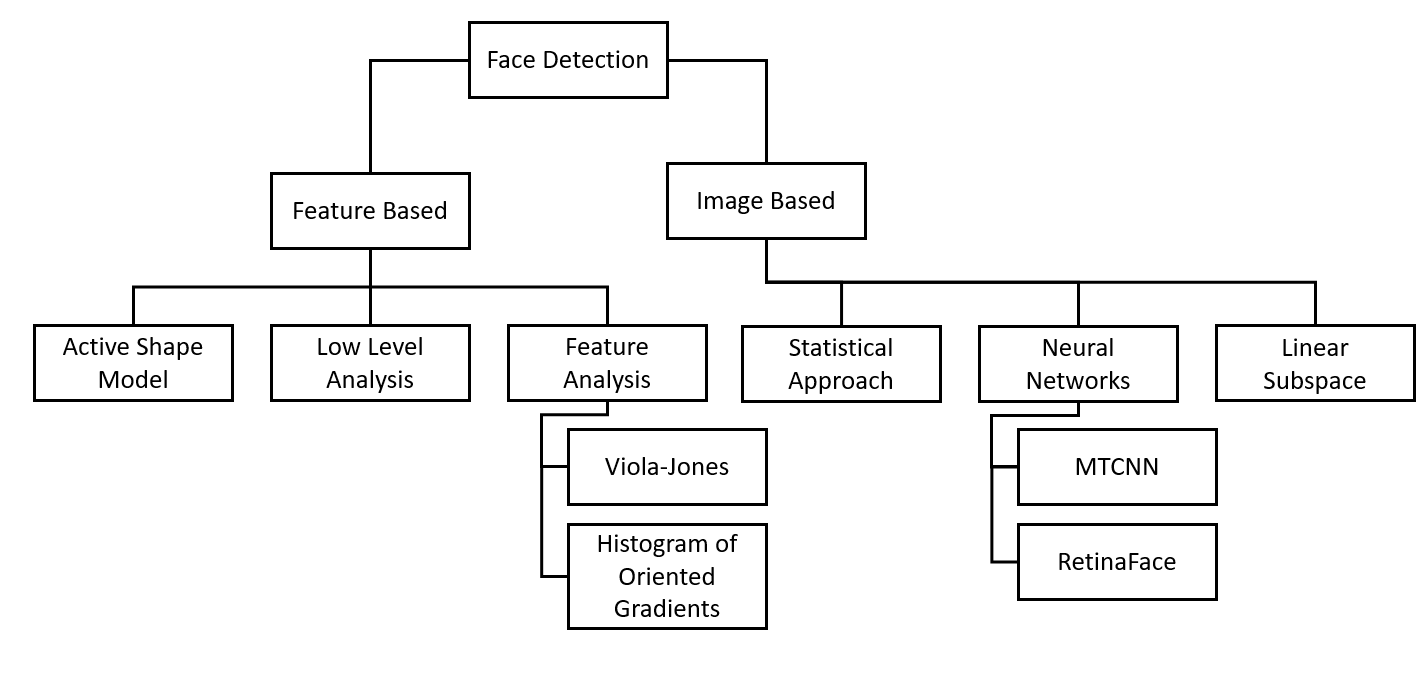
\includegraphics[width=\textwidth]{images/map.png}
    \caption{Diagram of face detection approaches modified from: Face Detection: A Survey (\cite{survey}).}
    \label{map}
  \end{minipage}  
\end{figure}
% \section{Face Detection Scene} 
% The computer vision field is a relatively young area of study within computer science. The major advancements for facial and object detection came at the turn of the century with the Viola and Jones paper in 2001 \cite{viola}. This paper proposed a method of detecting faces with little processing power. It used an integral image for the quick computation of its HAAR like features which were generated by comparing areas of intensity. This combined with the cascade structure meant the framework was efficiently able to detect faces with a low false positive rate. This foundational method for face detection was important in the scene of computer vision and helped lay the groundwork for future frameworks. 4 years later HOG \cite{hog} built upon this research by using features similar to Viola and Jones. Its features were calculated using a histogram based on the direction of gradients for an image. The HOG descriptor values could also be normalised over regions in the image which improved the robustness of the framework when given images of varying brightness. Both are still used today for their efficiency and simplicity and can be praised as the algorithms that helped dictate the direction of future work in the field.  
% Recently in the pursuit of accuracy there has been a domination of CNN and "deep learning" methods in the field that were aided with the rise of faster GPU's and more computational power, which the foundational methods didn't have. R-CNN \cite{rcnn} and MTCNN \cite{mtcnn} are two of these methods released recently. Although they both use CNN's they operate in different ways. R-CNN makes region proposals of bounding boxes on an image and then uses a deep CNN network to localise and segment the objects. MTCNN instead uses a cascaded multi-task network that predicts the bounding boxes and landmarks and then refines them through its 3 networks. It's multi-task learning improves its efficiency and performance. MTCNN and R-CNN are state-of-the-art algorithms that harness the advancements of deep learning. These algorithms are magnitudes more accurate than the 2 foundational methods (\cite{hog},\cite{viola}) but due to the complex structure of CNN's they are slow and computationally expensive.
% Generally most of the algorithms in the field can be put into two groups, feature extraction methods and deep CNN methods. Both have their positives and negatives and too truly understand if a bias exists in the field then it would be important to look at both groups.
\section{Types of Face Detection}
Face Detection: A Survey (\cite{survey}), details that face detection approaches can be placed into two distinct categories. These being feature-based methods and image-based methods, seen in figure \ref{map}. Both methods use a similar approach to detect faces by searching for features within an image. The difference comes from how the representation of a feature is encoded into the algorithms.
\subsection{Feature-Based}
\label{featurebased}
% the knowledge of face
% geometry has been employed to characterize and subsequently verify various features from
% their ambiguous state
% Most faces are of a similar shape so creating a filter that would search for this shape would allow for reasonable accuracy in face detection. Combining this filter with others that look for skin tone, or filters that use pixel intensities to find edges, would result in a stronger filter that could detect faces with more accuracy
 Feature-based detection is form of face detection that uses handcrafted filters that look for features in the image. These filters are created manually and leverage the pre-existing knowledge into the facial domain to understand what features can be extracted from the image. The knowledge of the facial domain consists of understanding things such as the geometry of features, regions of brightness and other hidden structures that are present in faces. These shared characteristics of the face are encoded into a classifier that is trained to recognise them. If the classifier locates these features in an image. Then a face is detected. This type of face detection was a very popular method to detect faces as it was relatively easy to understand and implement. Many of the early detectors in the field of computer vision were feature-based detectors. They are still used today, combining with machine learning classifiers to become strong tools when it comes to face detection and classification. They are usually very efficient and accurate when the filters can match in the image. Although, due to their handcrafted design, they can fail spectacularly when the filters don't match. This results in a lack of robustness when using them in uncontrolled environments, where the faces could have different expressions, lighting and occlusion. These filters could be engineered to perform better in these circumstances but this becomes a difficult and complex task as the number of factors the filter has to be prepared for increases. 
\subsection{Image-Based}
\label{imagebased}
Image-based detection is another form of detection and is the category most of the current state-of-the-art detectors belong to. CNN and deep learning are both image based methods (\cite{mlm}). In this method the face detection is accomplished by using a convolutional neural network, which in its base form is a deep learning algorithm. It can take a set of images and understand the hidden structures and encodings within them automatically. This is done through the use of the convolution layer, which is where the the input image is multiplied by a set of weights, these weights are the filter. By training the algorithm with a dataset of annotated faces, to minimise the euclidean distance between predicted coordinates and ground truth coordinates. The weights and therefore filter, are altered in accordance to this learning problem. This means the weights/filter would eventually learn the task and be able to predict coordinates for landmarks and bounding boxes with accuracy. Unlike handcrafted detectors where the filter has to be created depending on pre-existing domain knowledge. The CNN method allows a filter to be learned and optimised automatically using a dataset and learning problem (\cite{mlmconv}). It is a very robust method and benefits from more data being fed into it to further improve its prediction accuracy. With the rise of faster GPU's, image-based methods dominate the face detection field.

\section{Algorithms}
\label{algorithms}
% This chapter discusses the 4 algorithms and how they work in regards to face detection and landmark detection. There are many more intricacies that are present in the algorithms that are not discussed as they do not relate to the early stage of face detection.
Following are the details behind the 4 algorithms that were evaluated for this project. The algorithms differ in structure and design. They were chosen based on their novel approaches to face detection, as they contained a variety of components present in the computer vision scene.
\subsection{Viola-Jones Algorithm}
\label{viola}
The Viola-Jones algorithm (\cite{viola}), is a foundational feature-based algorithm. It is one of the earliest algorithms in the field and the simplest. The ability to detect faces accurately and efficiently is why it is still being used today as a baseline comparison algorithm.
\begin{figure}[h!]
\centering
  \begin{minipage}{\textwidth}
  \centering

    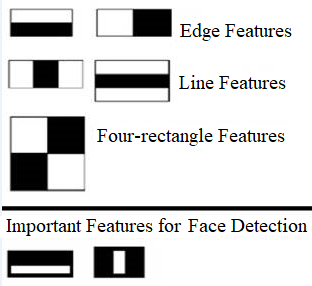
\includegraphics[width=0.5\textwidth]{images/haarlike_features.png}
    \caption{Haar-like features taken from: Towards Data Science (\cite{haarlikeimage}).}
    \label{haarlike_features}
  \end{minipage}  
\end{figure}

The algorithm works by using the pre-existing knowledge that features in a face vary in brightness. If the algorithm can find these features then it can classify the face. It does this by using haar-like features based on haar wavelets as described in \cite{haar}. These simple image features can be visualised as white and black adjacent rectangles as seen in Figure \ref{haarlike_features}. They are calculated by taking the difference of pixel intensities of adjacent regions in a rectangle in the image. For example, in a face the region around the eyes would usually be darker than the eyes themselves resulting in a haar-like feature for the eyes. In the same way that the centre of the nose would be brighter than the region around it, resulting in another haar-like feature which represents the nose. This is described in figure \ref{haarlike_features_face}, where the haar-like visualisations have been imposed over a face. This feature representation is what helps the algorithm understand what facial features it is seeing in an image.
 
\begin{figure}[h!]
\centering
  \begin{minipage}{\textwidth}
    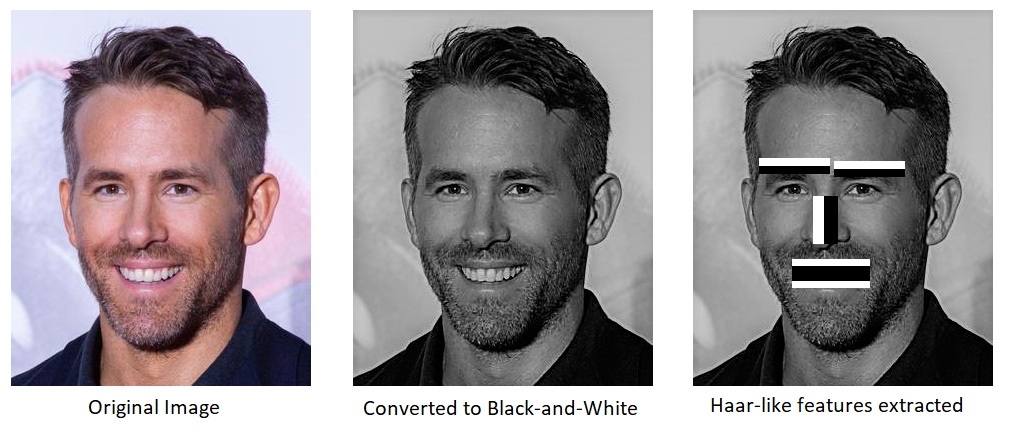
\includegraphics[width=\textwidth]{images/haarlike_features_face.png}
    \caption{Haar-like features imposed over face. }
    \label{haarlike_features_face}
  \end{minipage}  
\end{figure}

Computing these features can be costly which is why the Viola-Jones algorithm uses an intermediate representation for the image, called the integral image. This allows for quick calculation of the haar-like features by having every pixel represent the sum of every pixel to its left and above it. To extract a feature, the 4 corners of a region in the integral image can be used to calculate the pixel intensity difference for the whole region. This is more efficient then adding up each pixels intensity separately in the regions and subtracting them. 

To understand what haar-like features are the most important to classify a face, a strong classifier is created by combining weaker classifiers together through adaptive boosting. This works by starting at a weak classifier which used one feature to classify an image. This classifier was taken and another feature was added to it. The feature added to it was chosen based on how well it would compliment the previous classifiers feature. This meant that it was chosen based on the images the previous classifier got wrong, and what feature could best classify these images. This would increase the weight of the images the classifier had trouble with, and lead to optimising a strong set of features that classify a face.

The Viola-Jones algorithm uses a cascade of classifiers, where each classifier was trained with 9832 training faces and 10,000 non-face sub windows using the AdaBoost learning technique. The algorithm continually scans the integral image using a window looking for the most important general feature. If this haar-like feature is not present then the window can be rejected and classified as not containing a face. However, if the feature is present then the window moves to the next stage in the cascade, where another feature more specific than the previous is searched for. If this feature exists then the window again moves forward to the next stage. As the stages in the cascade continue, the haar-like features that are being searched for are more specific. If a window can go through every stage of the cascade without being rejected. Then every haar-like feature has been found, and the window contains a face. The cascade structure of the classifiers means that only the strongest candidate windows would reach the strongest and most computationally expensive classifiers. This method reduced the computation time drastically whilst improving the efficiency. 

% The classifier was trained using 4960 images that were manually annotated with faces and 9544 non-facial images. The cascade of classifiers introduced was a concept used in countless algorithms after the Viola-Jones paper. It worked by applying simple classifiers to the image first, these would reject many negative bounding box predictions so that only the strongest candidates would make it to the strongest and most expensive classifiers. This method reduced the computation time drastically whilst improving the efficiency. 

% This algorithm was heavily dependant on its feature extraction and only worked as a fully frontal face detector in very controlled situations as faces that were tilted or turned created problems for the algorithm to detect features for.
\subsection{Histogram of Oriented Gradients}
\label{hog}
The histogram of oriented gradients (\cite{hog}) is a popular feature based detector available through the DLIB library, which is a machine learning and data analysis toolkit (\cite{dlib}). The DLIB face detector can be broken down into 2 stages, a histogram of oriented gradients feature descriptor and a linear support vector machine classification algorithm. 

The detector works by using a histogram of oriented gradients to represent an image. As a feature descriptor, its purpose is to represent the image in a form that is easier for the computer to understand. By transforming the image into its gradients, the excess information is removed that the algorithm doesn't require like colour and background. These oriented gradients describe the edges in an image through the changes in intensity. 

To calculate the oriented gradients of an image. Two kernels are applied. These kernels output the respective horizontal and vertical gradients in the image according to the changes in intensity between the adjacent pixels around the target pixel. Using this information the gradient magnitude and orientation can be calculated for the horizontal gradient, \(g_x\) and vertical gradient, \(g_y\).
\[ g = \sqrt{g_x^2 + g_y^2} \]
\[ \theta = arctan (g_y/g_x) \]
The pixels can be represented as a combination of oriented gradients with both magnitude (\(g\)) and direction (\(\theta\)) associated with them.

\begin{figure}[h!]
  \centering
  \begin{minipage}{\textwidth}
  \centering
    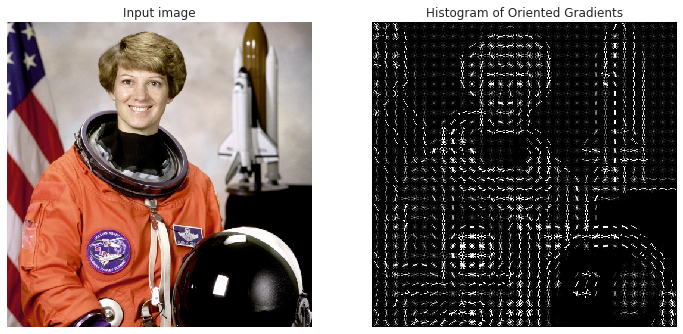
\includegraphics[width=0.7\textwidth]{images/hog_face.png}
    \caption{Histogram of oriented gradients representation from: Opengenus IQ (\cite{hogastro}).}
    \label{hog_face}
  \end{minipage}
  \hfill
\end{figure}

This results in an intermediary representation of the image with only its oriented gradients and magnitude as seen in figure \ref{hog_face}. Here the image can still be realised even though it doesn't have its other characteristics like colour and background.

The next step is to generate the histogram of these oriented gradients within the image. This works by looking at 8x8 blocks of pixels in the image and calculating a histogram of the gradients and directions. Each histogram consists of 9 bins of \(20^o\). The bin is chosen depending on the value of orientation, and the value placed within the bin is dependant on the magnitude. This is to say that if a pixel is halfway between two bins, then its magnitude is split evenly for each bin. If the pixel is closer to one bin than the other, then one bin will have a larger share of the magnitude.

Often the 8x8 blocks are very sensitive to lighting differences as some might be brighter than others. To reduce this variation 4 8x8 blocks are used to create a single 16x16 block. From this block, the 36x1 vector representing the histogram will be normalised. For a 36x1 vector, V:
\[V=[x_1,x_2,x_3,...x_{36}]\]
The normalisation factor k, would be the root of the sum of squares for each value:
\[ k = \sqrt{x_1^2,x_2^2,x_3^2,...x_{36}^2} \]
Resulting in the normalised vector being every value in vector \(V\) divided by the normalisation factor:
\[Normalised Vector = (\frac{x_1}{k},\frac{x_2}{k},\frac{x_3}{k},...\frac{x_{36}}{k})\]
This normalised vector would be calculated for all 16x16 grids in the image and combined to produce one large feature vector which would be trained with the SVM classifier to detect faces. If the classifier came across an image which resulted in a feature vector similar to a feature vector it had been trained to understand represents a face. Then the classifier would be able to classify that a face has been detected. This method uses the HOG descriptors as feature representations for the image, similar to how the Viola-Jones algorithm used haar-like features.

The landmark predictor present in the DLIB library is based on the algorithm from \cite{onemilli}. The landmark coordinates are predicted through the use of a predictor trained on the 68 point i-BUG dataset (\cite{300w}). An initial prediction of the 68 points are generated based on the mean of the training data scaled by the bounding box. This prediction is then altered by a slight amount and updated continuously based on adjacent pixel intensities to help regress the 68 points to their most accurate positions.
% \begin{figure}[h!]
%   \centering
%   \begin{minipage}{0.6\textwidth}
%     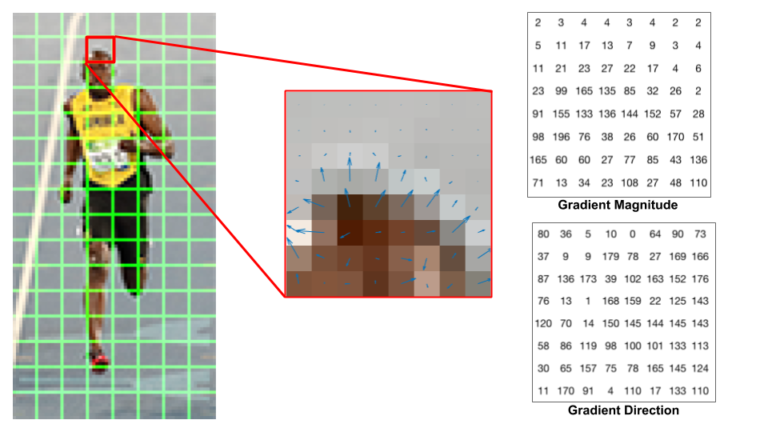
\includegraphics[width=\textwidth]{images/hog_split.png}
%     \caption{Average Error Values Across Algorithms}
%     \label{hog_split}
%   \end{minipage}
%   \hfill
% \end{figure}
%talk about 68 point detector

\subsection{Multitask Cascaded Convolution Networks}
\label{mtcnn}
The MTCNN algorithm is an image-based CNN algorithm which leverages interesting design to improve its accuracy and efficiency (\cite{mtcnn}). It uses 3 different neural networks to perform bounding box calibration, face landmark localisation and face classification. The proposal network (P-Net) is used to propose bounding boxes and performs non-maximum suppression. The refine network (R-Net) is used to refine the bounding boxes through bounding box regression and NMS. The final output network (O-Net) is used to output the five facial landmarks present in the face. These 3 networks are visualised in figure \ref{mtcnn_pipeline}
\begin{figure}[h!]
  \centering
  \begin{minipage}{\textwidth}
  \centering
    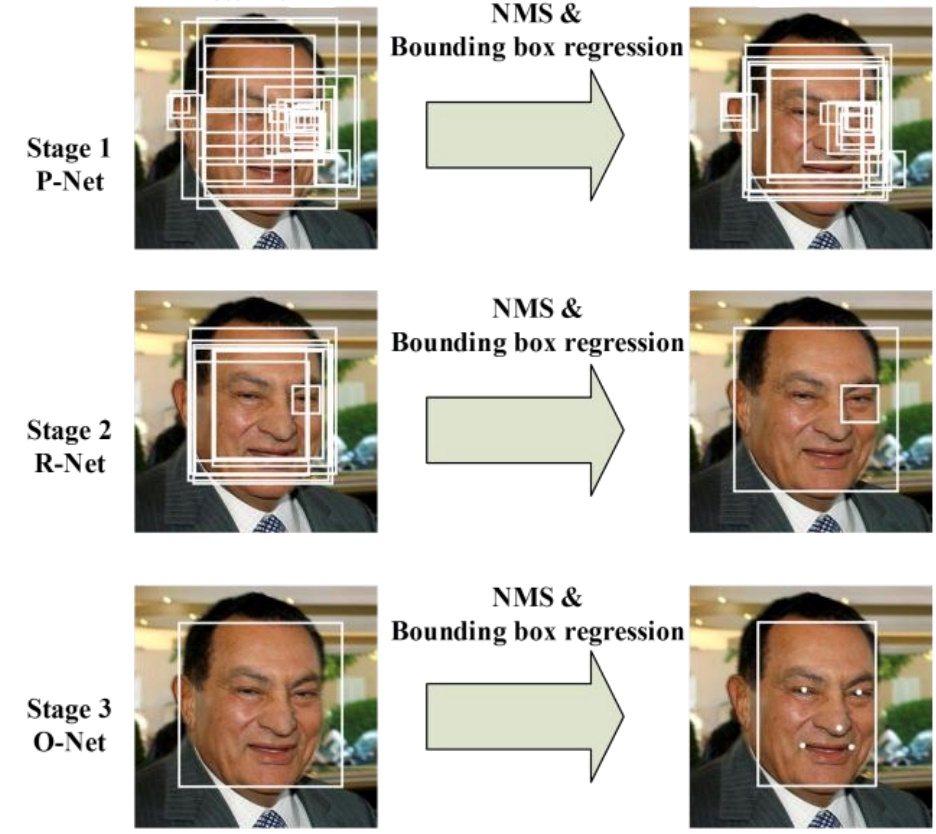
\includegraphics[width=0.4\textwidth]{images/Inkedcropped_mtcnn_pipeline.jpg}
    \centering
    \caption{MTCNN pipeline modified from: Joint Face Detection and Alignment using Multi-task Cascaded Convolutional Networks (\cite{mtcnn}).}
    \label{mtcnn_pipeline}
  \end{minipage}
  \hfill
\end{figure}

The algorithm uses a sliding window to scan through the image and send 12x12 pixel sized regions to the first neural network, the P-Net. Although, before it can do this the image is first re-scaled to create an image pyramid. This is a series of the image all scaled to smaller sizes. The reasoning behind scaling the input image to different sizes is too reduce the complexity and allow the larger faces to be scaled down to a size that the scanning window can recognise, as well as maintain the larger image so that smaller faces within it can be identified. This is illustrated in figure \ref{ip}, where the sliding window cannot recognise the original scale face as it is too large for the window. However, when the image is scaled down through the image pyramid. The sliding window is able to detect the presence of a face as it fits within the window size. This is an important step as it allows faces of different sizes the opportunity to be correctly recognised by the first network. 
\begin{figure}[h!]
  \centering
  \begin{minipage}{0.9\textwidth}
    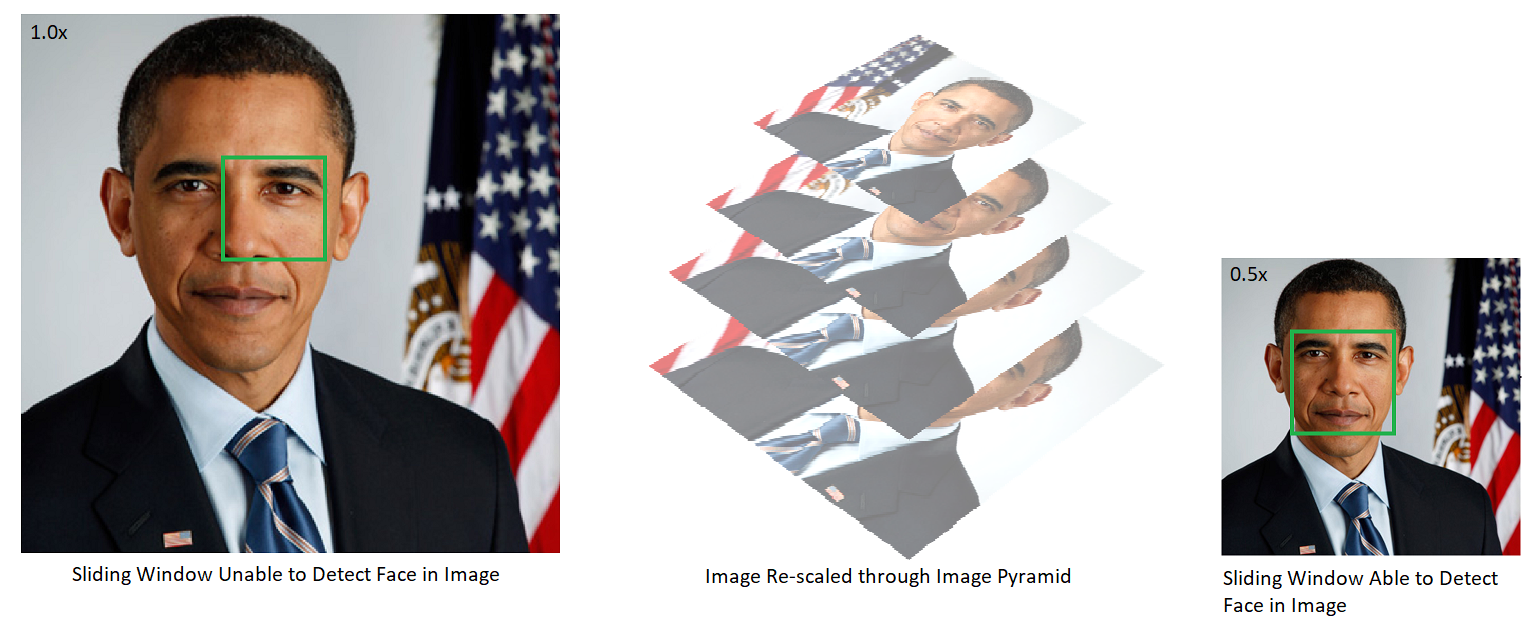
\includegraphics[width=\textwidth]{images/ip_better.PNG}
    \caption{Image pyramid re-scaling image for detection window.}
    \label{ip}
  \end{minipage}
  \hfill
\end{figure}

The P-Net proposes the first set of bounding boxes it detects in the image. Each box has a confidence score assigned with it, which relates to how confident the algorithm is that its successfully detected a face. To reduce the computational effort in the later networks, any bounding boxes with low confidence scores are removed. This reduces the number of candidates, but to further reduce them, non-maximum suppression occurs. This sorts the candidate bounding boxes by their confidence score and removes those candidates which have a large overlap with other higher confidence candidates. This means that the P-Net outputs a list of bounding boxes the network is most confident in. These are re-scaled and fed into the next network, the R-Net. This network performs similarly to the P-Net and looks to regress the bounding boxes to more accurate coordinates, as well as reduce even more candidates through NMS merge. The final network takes the bounding boxes returned by the R-Net and predicts the landmark locations and a confidence level for each box. Boxes with a lower confidence level are removed and NMS occurs. This should result in each face detected having a single bounding box and set of landmarks associated with it.

Each layer of the network is trained differently. The P-Net is trained using randomly selected images from the WIDER FACE (\cite{widerface}) dataset for classification and the CelebA dataset (\cite{celeba}) for landmark localisation. The R-Net is trained using the P-Net's detected faces from WIDER FACE for face classification and detected faces from the CelebA dataset for landmark localisation. The final network O-Net is trained similarly to the R-Net but both classification and landmarks localisation is trained on faces detected with P-Net and R-Net from WIDER FACE and CelebA respectively. 

\subsection{RetinaFace}
\label{retinaface}
RetinaFace is a single shot image-based detection method which has the goal of accurate detection of multiple faces in a image (\cite{retinaface}). Single shot means that the method doesn't use the two stage architecture of proposal and refinement in which coordinates are proposed and rejected, but instead predicts directly from its feature maps through pixel-wise face localisation. This results in an efficient algorithm as there is no time consuming proposal stage.

\begin{figure}[h!]
  \centering
    \begin{minipage}{0.49\textwidth}
    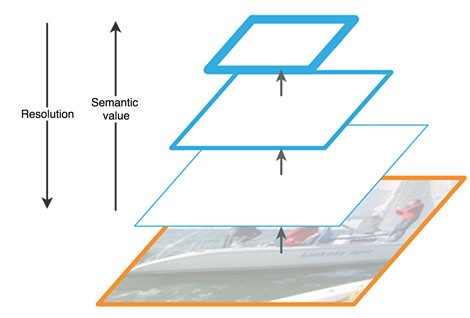
\includegraphics[width=0.94\textwidth]{images/fp_semantics.jpeg}
     \vspace*{-0.6mm}
    \caption{Feature pyramid network semantic value and resolution from: Medium (\cite{fpnsemantic}).}
    \label{fpnsemantic}
  \end{minipage}
  \hfill
  \centering
  \begin{minipage}{0.49\textwidth}
    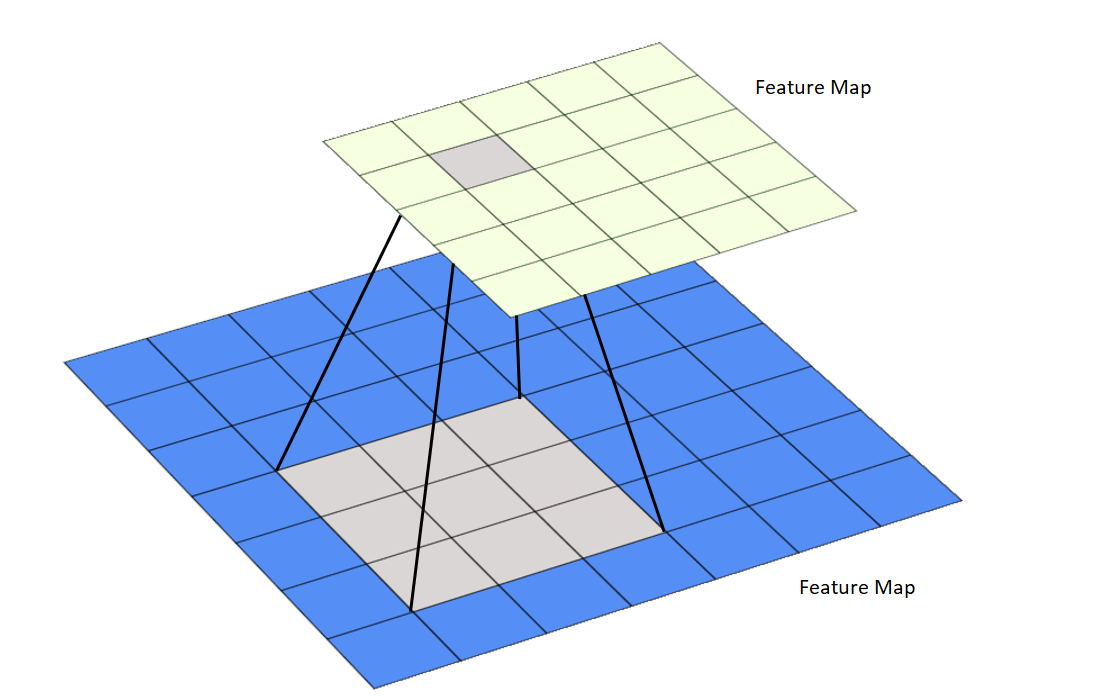
\includegraphics[width=\textwidth]{images/fp_scaling.PNG}
    \caption{Diagram showing how semantic information is increased through layers of pyramid.}
    \label{fp_scaling}
  \end{minipage}
  \hfill
\end{figure}
It uses a CNN method which utilises 3 main components. A feature pyramid network, context head module and cascade multitask loss. From these 3 components the most important to understand for RetinaFace is its feature pyramid network.
% \begin{figure}[h!]
%   \centering
%   \begin{minipage}{0.5\textwidth}
%     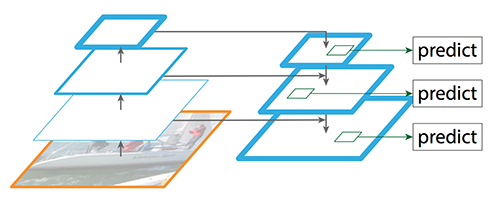
\includegraphics[width=\textwidth]{images/fp_lateral.png}
%     \caption{Feature Pyramid Network Up-sampling and Down-sampling Structure from: Feature Pyramid Networks for Object Detection
% (\cite{fpn}) }
%     \label{ip}
%   \end{minipage}
%   \hfill
% \end{figure}
% \begin{figure}[h!]
%   \centering
%     \begin{minipage}{0.49\textwidth}
%     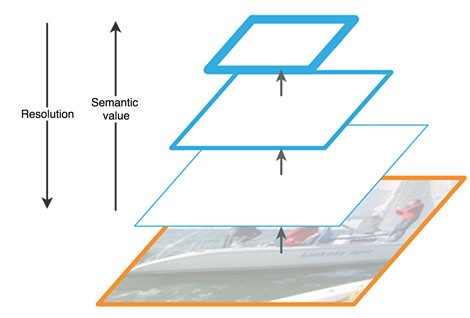
\includegraphics[width=0.94\textwidth]{images/fp_semantics.jpeg}
%      \vspace*{-0.6mm}
%     \caption{Feature Pyramid Network Semantic Value and Resolution from: Medium (\cite{fpnsemantic})}
%     \label{fpnsemantic}
%   \end{minipage}
%   \hfill
%   \centering
%   \begin{minipage}{0.49\textwidth}
%     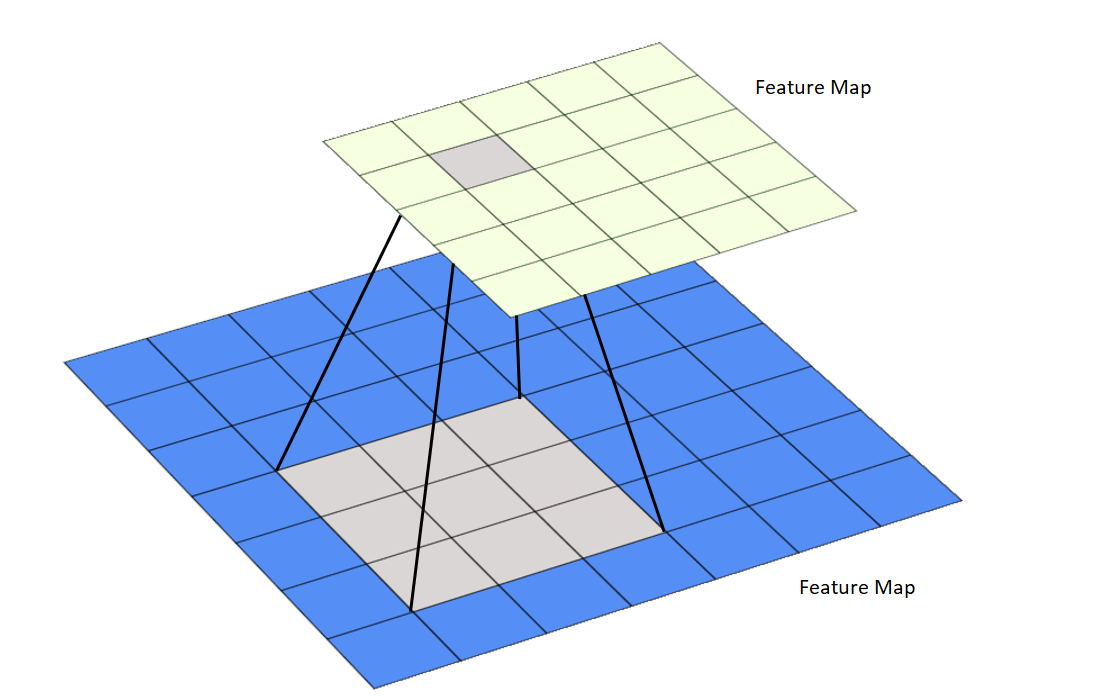
\includegraphics[width=\textwidth]{images/fp_scaling.PNG}
%     \caption{Diagram showing how Semantic Information is Increased through Layers of Pyramid}
%     \label{fp_scaling}
%   \end{minipage}
%   \hfill
% \end{figure}
The feature pyramid is similar to an image pyramid in only its shape. The difference is that in an image pyramid, the image itself is scaled to different sizes and features are extracted from each scale. This can be time consuming when it comes to training the algorithm and it often requires a large amount of memory for the multiple scaled images it has to store. A feature pyramid instead generates feature maps for the single scale image and then uses those feature maps to generate different sized feature maps as seen in figure \ref{fpnsemantic}. A feature map is the output of applying a filter on an input image. Through figure \ref{fp_scaling}, it can be seen that the structure of the feature pyramid network results in each layer taking its previous layer and reducing its size, but by doing so, also compressing the information from one feature map into the smaller output feature map. This means that each subsequent layer in a bottom-up approach has a lower resolution but more semantic information contained within it.

The RetinaFace algorithm uses these lower resolution, high level feature maps to detect faces. The layers with more semantic information can be used to reconstruct higher resolution feature maps which can then be used to make predictions of faces and landmarks. Due to the upsampling and downsampling, the location of faces within an image wont be precise. To solve this there are lateral connections between feature maps and their reconstructed counterparts at each layer. This helps the reconstructed layers with precise location and assists the detector in making more accurate predictions (figure \ref{ip_lateral}).
\begin{figure}[h!]
  \centering
  \begin{minipage}{\textwidth}
  \centering
    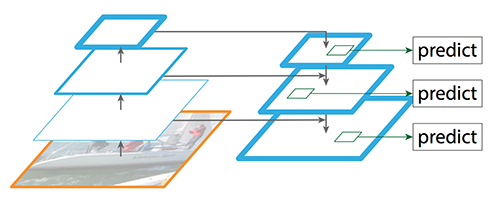
\includegraphics[width=0.7\textwidth]{images/fp_lateral.png}
    \caption{Feature pyramid network upsampling and downsampling structure from: Feature Pyramid Networks for Object Detection
(\cite{fpn}). }
    \label{ip_lateral}
  \end{minipage}
  \hfill
\end{figure}

% The context module provides extra contextual information on top of the outputs of the FPN through the use of deformable convolutional networks (\cite{dcn}). It makes predictions and outputs regression parameters. The first context head module starts by predicting the bounding boxes using the original boxes. Then the second context head module adjusts the boxes using the regression parameters outputted by the first context head module to predict an accurate bounding box and landmark coordinates.

The RetinaFace algorithm is trained using the WIDER FACE dataset (\cite{widerface}), which contains 32,203 images and 393,703 annotated bounding boxes. The five facial landmarks of nose, eyes and mouth edges have been manually annotated onto this dataset to train the algorithm for landmark detection.
\section{Bias Existing}
\label{bias}
There are many notable cases of facial analysis algorithms performing in a biased way and due to the rise of this emerging technology, these cases are becoming more common. In 2017 with Apple's new iPhone X launch, came their new Face ID feature which used faces as biometric security. Their implementation created issues as it was reported that in China the facial detection was under performing. It was unable to distinguish faces correctly, and would unlock the phone under falsely identifying someone as the correct user (\cite{iphone}). This problem was only evident in China indicating a bias towards race. Another example is Amazon's face recognition system called "Rekognition", mismatching members of the American congress to mugshots of criminals (\cite{amazon}). This was criticised on the fact that 40\% of the mismatched faces belonged to 20\% of the people of colour. These disproportionate results indicated the underlying bias present in the company's system. At a larger scale the UK Home Office implemented a new passport checking service, in which the users face would be detected and compared against a database of faces to match faces to passports. The system failed as the facial detection didn't work upon very light or dark skin tone individuals (\cite{passport}). This was a technology that was approved and introduced into real world use which had a major bias present within it. It is evident there are many cases of this bias existing, and with the current use cases of face detection in law enforcement and hospitals. The existence of bias would cause major repercussions for the targeted groups.
\section{Previous Work}
Since the mainstream introduction of computer vision technologies, only recently has there been dialogue in recognising the existence of bias within them. Therefore, there are not many published papers available that directly research this bias. However, there are a few pieces of literature that stand out.
\subsection{Gender Shades}
The Gender Shades paper (\cite{gendershades}), discusses an approach to evaluate bias present in facial analysis algorithms in regards to race and gender. They evaluated 3 commercial classifiers from Microsoft, IBM and Face++. They found that all classifiers performed better on male faces than female faces, and all classifiers performed better on lighter faces than darker faces. This led them to believe that single performance metrics are occlusive to the field and industry because the classifiers they tested all had accuracy values ranging from 87.9\% to 93.7\%. This meant that the classifiers could be described and marketed as accurate, but as their results indicated this accuracy broke down completely when it came to females and darker skin tones. They also recognized the lack of datasets available in which phenotypic features such as skin tone were labelled. Understanding that the lack of datasets causes a large training bias, they constructed the Pilots Parliamentary benchmark dataset. It consisted of 1270 parliamentary subjects that were evenly distributed in regards to gender and skin colour. This paper is important as it discusses many of the issues with bias and ultimately shows that it exists for even the largest tech companies algorithms. Being a recent paper from 2018 means that there is a lot of work left to do for facial detection to be used fairly in the wild.
\subsection{IBM: Diversity in Faces}
IBM's Diversity in Faces (\cite{dif}), proposed a new unbiased dataset by providing a diverse large annotated face dataset to train and evaluate algorithms. In this paper diversity isn't reduced to only ethnicity or gender, which some other datasets conclude is representative. Instead diversity is put down to 10 different coding schemes which include gender, age, skin colour, facial symmetry and different craniofacial differences. This dataset looks to have an even distribution of faces according to their different coding schemes. They found that this approach to diversity would mean a largely unbiased dataset as diversity was being statistically measured to ensure that the different factors that made faces diverse were being evenly distributed. This paper also evaluated other popular datasets available. They found that these datasets like IJB-C (\cite{ijb-c}) and AgeDB (\cite{agedb}), were heavily skewed towards containing a smaller percentage of darker skin tone faces and females. This emphasised the need for their fairer dataset. The paper made a large step in addressing the bias present in training data, and helping advance the study of fairer datasets.
%Algorithms training on this type of dataset would perform with much less bias as its not inherently being introduced at the training stage so any bias that exists would be within the algorithm itself
\subsection{Pride or Prejudiced?}
Deep Learning for Face Recognition: Pride or Prejudiced? (\cite{prideorpre}), looked to develop a deeper understanding into the bias of deep learning face recognition systems, and if the bias existing in the deep networks was similar to that of the bias within the human brain. The key findings of their research included that when a deep learning network is trained upon data representative of real world situations, such as a lack of exposure to specific races/ages. Then the network would show in-group bias across these characteristics similar to how humans would. Their experiments also indicated that in the case of two separate sets of images for two different races. That training a model on one race would always result in worst performance for images of the other. The paper analysed the bias existing with deep learning methods, and looked specifically into the datasets as opposed to the components of the network. This brought forward the conclusions that there are benefits in using larger datasets to improve performance. However, it is not a complete solution to remove bias in regards to race and age.
\subsection{Role of Demographic Information}
Face Recognition Performance: Role of Demographic Information (\cite{demographic}), looked at 3 more commercial face recognition algorithms and evaluated their performance against a dataset labelled with race, ethnicity, gender and age. The results of the study found that females in the black and younger groups were harder to recognise for every algorithm. They found that training the algorithms with images of faces that are well distributed across the groups is very important in reducing the difficulties for recognising the specific groups. This paper was published in 2012 and shares many relevant findings with the 2018 Gender Shades paper. This shows that within a six year gap there hasn't been a considerable improvement in reducing bias at a large scale, even though the problem has been evident for years.
%==================================================================================================================================

\chapter{Implementation}
\label{implementation}
This chapter discusses the brief set of requirements and implementation details behind the 4 algorithms that were used for this projects research. 
\section{Requirements}
When implementing the different algorithms there were certain requirements that had to be kept in mind. These requirements were formulated based on the research question. They describe the minimum required from the implementation, so that it can be evaluated to see if there exists a bias.
\begin{itemize}
  \item Algorithms must provide bounding box coordinates.
  \item Algorithms must provide landmark locations.
  \item Open source implementations used must not differ from the training described in the original papers.
\end{itemize}
Requiring the implementations to provide bounding box coordinates and landmark locations is necessary as this is the first stage of detection, and the coordinates are required to indicate accuracy. Ensuring that the implementations used weren't trained on other datasets was also necessary, because evaluation of the algorithms training data would be harder if they were fine tuned with out explicitly stating so.
\section{Notebooks}
The algorithms were implemented within the Google Colab environment. This is a cloud based Python notebook that allows for quick execution of code and provides a GPU memory allocation for any machine learning tasks. Each algorithms implementation was self-contained in its own notebook as they used an assortment of libraries and modules which would've caused compatibility issues if present in the same notebook.
\subsection{Viola-Jones Algorithm}
The Viola-Jones algorithm is implemented using the OpenCV Python library (\cite{opencv}), which consisted of useful Python bindings that assisted in computer vision and more specifically, face detection tasks.

To run the algorithm, the pre-trained haar cascade classifier present in the OpenCV library is instantiated. Accessing the frontal face classifier allows the face detector to detect faces that are fully frontal facing because this is what the classifier has been trained for. The image is imported into the notebook through OpenCV. This imports the image as a colour image in the BGR colour mode. Since the classifier doesn't require colour, the image is converted to gray scale. To call the detector, the \textit{detectMultiScale()} function is called with an image as a parameter. This returns an array of length 4 that contains the bounding box values. These values are bounding  box's x and y coordinate of the top left point, along with the height and width. Using these 4 values, the coordinates of the 4 corner points on the bounding box can be obtained. The bounding box values for each image are placed into a dictionary and exported as a JSON file for further analysis.

The Viola-Jones algorithm doesn't output landmark locations because the filter is only trained to classify faces and output bounding boxes. There are smile classifiers and eye classifiers available through the OpenCV library, these could be used to get the location of landmarks. However, these filters only place a box around the feature instead of returning a coordinate point. The lack of precision and not being discussed in the original paper is why these filters weren't considered for the implementation.
\subsection{Histogram of Oriented Gradients}
The 68 point HOG detector implementation is heavily inspired from Adrian Rosebrock's blog (\cite{68p}), in which he discusses a method to detect facial landmarks using DLIB, OpenCV and Python.
\begin{figure}[h!]
  \centering
  \begin{minipage}{0.5\textwidth}
    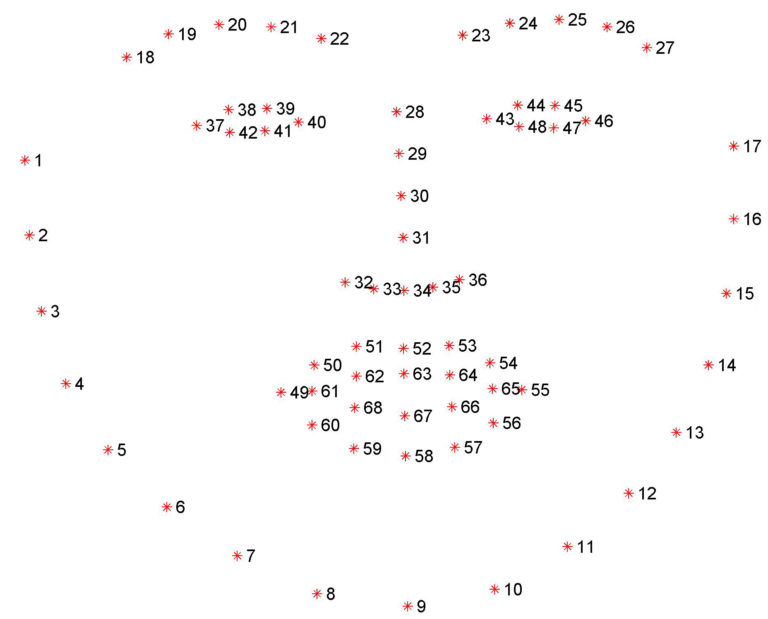
\includegraphics[width=\textwidth]{images/68point.jpg}
    \caption{Positioning of the 68 landmark coordinates from: Py Image Search (\cite{68p}).}
    \label{68p}
  \end{minipage}
  \hfill
\end{figure}

The model being used has been trained on the iBUG dataset (\cite{300w}), which consists of face images annotated with 68 points, these are visualised in figure \ref{68p}. This model will predict coordinate points around the face and landmarks creating a mask. First the 68 point pre-trained model is downloaded and instantiated as the predictor through the dlib \textit{shape\_predictor function()}. The face detector is also instantiated using the \textit{get\_frontal\_face\_detector()} function. This function initialises the HOG + SVM detector that DLIB has altered to work with face detection as opposed to general object detection. Similar to the haar cascade classifier, the DLIB detector doesn't require the images colours, so each image is transformed into gray scale. The instantiated detector is called on an image, which returns a rectangle object that contains the 4 values to describe the bounding box points. The predictor is then called which takes the image and calculated bounding box, and returns the predictions on the 68 coordinate points within a shape object. The helper function transforms the shape object to a numpy array for easier manipulation.

The 68 point detector varies in point selection from the 5 point detectors. This is because the eye landmarks which sit in the centre of the eyes are not present in the 68 point predictions. These points are important because they are two of the five landmarks present in the other algorithms. The predictor does make predictions for points on the edges of the eye as seen by points 37,40,43 and 46 in figure \ref{68p}. This means that an estimate of the eye landmarks can be generated. This estimate is created by taking the midpoint between the line connecting the edge points for each eye. It should indicate the centre of the eye with reasonable accuracy. The nose and mouth landmarks are present in the 68 point model, so these are extracted from the 68 points predicted. The 5 landmark coordinates and 4 bounding box values are placed in a dictionary of structure seen in figure \ref{dict}. This is then exported to a JSON file for further analysis.

%The structure of the dicutoanry
\begin{figure}[h!]
  \centering
  \begin{minipage}{0.8\textwidth}
    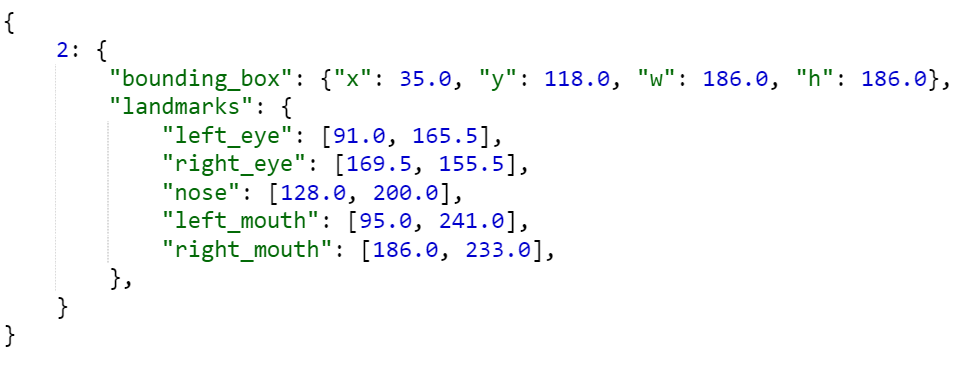
\includegraphics[width=\textwidth]{images/dictionary_structure.PNG}
    \caption{Dictionary structure of bounding box and landmark coordinates.}
    \label{dict}
  \end{minipage}
  \hfill
\end{figure}

\subsection{Multitask Cascaded Convolution Networks}
The algorithm is implemented through a Pytorch implementation of the pre-trained MTCNN face detection model available on Github (\cite{mtcnngit}). Using the infer notebook supplied on the repository provided a solid base to set the algorithm up. The implementation heavily followed the steps detailed within it.

First the MTCNN module is instantiated with its specified parameters. These include the minimum face size, image pyramid scaling factor, thresholds and margin. All the parameters besides image size remain at their defaults values. The image size parameter was set to 300. This was to ensure the best results, as the images it would be evaluated against would be of 300 width.

A loader object is then instantiated that is  used to load in the images into the algorithms detection stage. For every image in the loader the \textit{detect()} method is called on it, with the landmarks parameter set to true. This returns bounding box values, landmark locations and a probability value. The probability value is a number between 0 and 1 indicating how confident the algorithm is in its prediction. The bounding box values returned aren't of the standard form of x,y,w,h but instead are the x,y values of the top left and bottom right coordinates in the bounding box. To put these into the standard form of x,y,w,h. The height and width is calculated using the distance between the coordinates, and stored alongside the x and y coordinates of the top left point. The bounding box values along with the landmark locations are placed into a dictionary (figure \ref{dict}), which is exported as a JSON file.
\subsection{RetinaFace}
The RetinaFace algorithm is implemented based on a PyTorch implementation on Github (\cite{retinagit}). The detection is very simple and all that is required is the pre-trained model. This pre-trained model is trained on the WIDER FACE (\cite{widerface}) dataset as stated in the RetinaFace paper (\cite{retinaface}). It is downloaded through the \textit{get\_model()} function and is instantiated as the model with the parameters of max size set to 300. The max size is set to 300 to improve the performance of the algorithm. Every image is of 300 width with varying height to maintain its ratio. This means that setting the max size to 300 allows the same model to be used for every image and provide consistent results. After the model is set, face detection can be carried out by calling the \textit{predict\_jsons()} function on each image. This returns a list of dictionaries for every face it detects. Each dictionary contains the bounding box coordinates of the top left and bottom right points, as well as the landmark coordinates. The bounding box coordinates are used to generate the height and width, so that they can be stored of the form x,y,w,h in the output dictionary (figure \ref{dict}),
alongside the landmarks. This dictionary is then exported as a JSON file.
%Include section discussing evaluation notebook and problems encountered throufh proejct
\chapter{5025 Dataset}
\label{dataset}
This chapter discusses the motivation and design methodology behind the novel 5025 dataset. With in depth discussion on design decisions and limitations of the dataset.
\section{Motivation}
\label{datasetmotivation}

Throughout the course of the project it was realised that a dataset would be required to evaluate the performance of the algorithms. The motivation was to obtain a dataset that had an evenly distributed number of different races and genders, such that the accuracy of the algorithm could be compared between the different groups within the dataset. This annotated dataset was called the 5025 dataset and consisted of the images seen in figure \ref{5025}.
\begin{figure}[h!]
  \centering
  \begin{minipage}{\textwidth}
    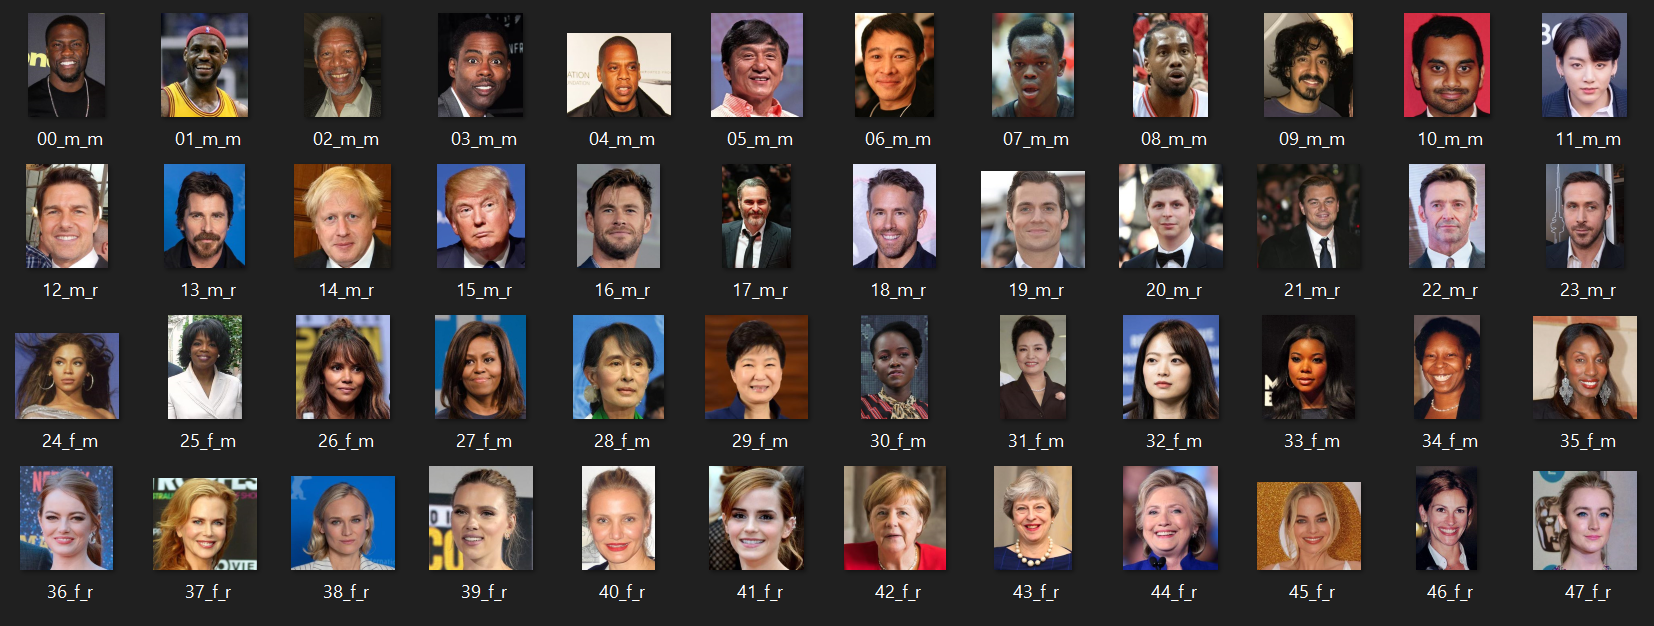
\includegraphics[width=\textwidth]{images/dataset.PNG}
    \caption{Images of 5025 dataset.}
    \label{5025}
  \end{minipage}
  \hfill
\end{figure}
\section{Design}
\label{datasetdesign}

\subsection{Pre-existing or Novel}
There were many considerations into the design of the dataset. The largest being whether to use a pre-existing dataset or compile a new one. Due to previous research being completed on understanding the bias within facial analysis algorithms, there existed datasets that contained faces of varying gender and race along with annotations labelling these aspects. These datasets were detailed in other papers such as Gender Shades (\cite{gendershades}) and FairFace (\cite{fairface}). Using these would be a valid approach as the annotations relate specifically to race and gender, which would allow the dataset to be split into distinct groups for evaluation. However, there is a lack of response in requesting many of these datasets which reduces their viability. There also exists difficulties coming from the variance of photos in the dataset. Often these images are taken in the wild, meaning that considerable effort would be required to comb through the datasets for images that were of little variance. Therefore, to allow for more control of every aspect of the dataset, a novel one was created.
\subsection{Dataset Diveristy}

To ensure the dataset was diverse and valid for evaluating if a bias was present, the judgement was made that the two factors of race and gender would be combined evenly into two categories. Represented and underrepresented faces. These categories better described the different races and genders that could be affected by bias, whilst maintaining two distinct groups. Gender was limited to males or females, and was split equally between the two categories. Race however wasn't limited the same way. Looking towards a specific race or by extension skin tone, would result in many groups in the dataset. To overcome this, race was generalised by using the idea of representation. Representation would consider how well a race was represented in the available datasets, and it would be placed in the corresponding group. This allowed for multiple races to be categorised in the dataset under the two groups. Underrepresented faces were faces considered to be underrepresented in benchmark datasets, which resulted in African American, South Asian and East Asian faces present. Whereas represented faces contained those of mainly European and American Caucasian faces, which are prevalent as the majority of faces in benchmark datasets. By considering race not as discrete races but as a continuous spectrum, allowed multiple races to be categorised into each group. This ensured the dataset was diverse, whilst maintaining it's ability to assess if a bias was present with race and gender.


% Both categories contained an equal number of males and females. This was done to maintain fairness in the categories.



% Gender was limited to males or females such that both categories had an equal number of genders. Race wasn't limited in the same way. Instead of looking towards a specific race or by extension skin tone, the goal was to generalise race by using the idea of representation. Representation would consider how well a race was represented in the data and it would be placed in the corresponding group. This allowed for multiple races to be represented in the dataset under the two groups. Underrepresented faces were faces considered to be underrepresented in benchmark datasets, which resulted in African American, South Asian and East Asian faces present. Represented faces contained those of mainly European and American Caucasian faces. It was important to consider race not as discrete races but as a continuous spectrum and therefore include multiple races under the underrepresented group, as when looking for a bias to do with race, its important to look at more than just one singular race.


% Both categories contained an equal number of males and females. This was done to maintain fairness in the categories.


% Race was the other important factor to consider. Instead of looking towards a specific race or by extension skin tone, the goal was to generalise race by using the idea of representation. Representation would consider how well a race was represented in the data and it would be placed in the corresponding group. This allowed for multiple races to be represented in the dataset under the two groups. Underrepresented faces were faces considered to be underrepresented in benchmark datasets, which resulted in African American, South Asian and East Asian faces present. Represented faces contained those of mainly European and American Caucasian faces. It was important to consider race not as discrete races but as a continuous spectrum and therefore include multiple races under the underrepresented group, as when looking for a bias to do with race, its important to look at more than just one singular race.
\subsection{Collation of Images}
There were multiple ways to collate the images. These being through Google Images, pre-existing datasets or manually capturing images.
The latter would have involved taking photos of participants belonging to represented and underrepresented groups within a controlled environment. It would provide the most control over the images but due to ongoing Covid-19 pandemic, it wasn't viable. The second option would've been to comb through the datasets that were available and select faces belonging to a specific race or gender, such that there was an even distribution. The problem with this was that many of the datasets were not labelled with race or gender, which combined with their large number of images, made it difficult to automatically or manually extract images of specific race or gender from them. The option of Google Images was chosen to collate dataset photos. When choosing the photos, it was ensured that they were of creative commons licence and that the photos had relatively little factors that would impact them in comparison to others. These factors included expression, illumination, shadows, occlusion and pose, as described in \cite{expression}. Minimising the differences was important in ensuring a fair evaluation of each group in regards to only race and gender.  The images were collated with the goal to ensure faces were fully frontal facing and showed little variance. To increase the number of available photos to select from, celebrities and public figures were specifically searched for, as they would have more photos available of them due to their significance. It was difficult to minimise the variance in the photos when capturing them from Google Images because the photos of the celebrities were taken under different conditions. To counteract this the photos were cropped and aligned manually. Faces showing neutral or smiling expressions and images that didn't have radically different lighting conditions were also specifically chosen to reduce variance. To further bring consistency to the dataset, the collated photos were resized so that every image was of 300 pixel width whilst maintaining the same aspect ratio. This ensured that the results wouldn't be skewed depending on the size of each face.
% The latter wasn't viable due to the ongoing Covid-19 pandemic. This method would have involved taking photos of participants belonging to represented and underrepresented groups within a controlled environment. It would

\subsection{Technical Details}
The dataset consisted of 48 distinct faces. Each image had a width of 300. This was decided by using the smallest width image and resizing every other image to match its width whilst maintaining the same aspect ratio. There were 24 represented faces and 24 underrepresented faces. Both these groups contained an equal number of males and females at 12 each. Each image was labelled following the scheme: \[ ID\_GENDER\_GROUP \] The ID was the face id ranging from 0 to 47, the gender was assigned either "m" or "f" indicating male or female and the group was assigned "m" or "r" indicating underrepresented or represented. 

\subsection{Annotations}
\begin{figure}[h!]
  \centering
  \begin{minipage}{0.8\textwidth}
    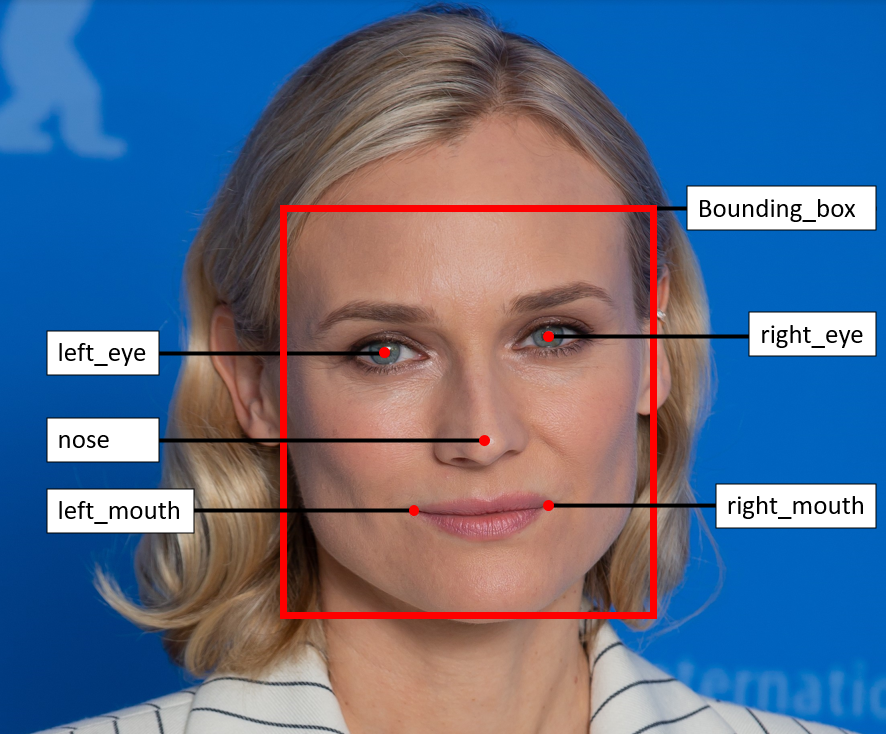
\includegraphics[width=\textwidth]{images/example_bb_better.PNG}
    \caption{Different landmarks annotated for each face.}
    \label{example_bb}
  \end{minipage}
  \hfill
\end{figure}
The dataset was annotated to provide a ground truth for the bounding box and landmarks. This consisted of annotating coordinates for the 5 landmarks and bounding box present for a face. The 5 landmarks consisted of the 2 eye landmarks, the nose landmark and the 2 mouth landmarks. The bounding box annotations were the x,y coordinates denoting the top left corner of the bounding box, along with the corresponding height and width in pixels. These annotations can be seen visualised in figure \ref{example_bb}
% \begin{figure}[h!]
%   \centering
%   \begin{minipage}{0.8\textwidth}
%     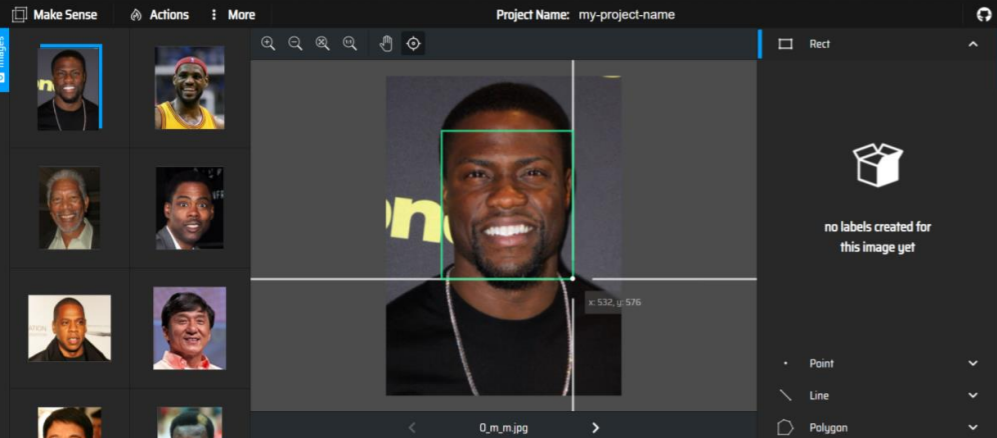
\includegraphics[width=\textwidth]{images/makesense.PNG}
%     \caption{MakeSense.ai Interface for Creating Manual Annotations}
%     \label{makesense}
%   \end{minipage}
%   \hfill
% \end{figure}

They were generated manually through the use of MakeSense.ai (\cite{makesense}), which is an online tool that provided a graphical interface to place points on each image and export the resulting coordinates as a CSV file. Manual annotation was chosen because each point could be placed accurately. With only 48 images, this task viable and not time consuming. A collaborative method was considered that would allow participants to annotate the images, which would then be averaged and used as the ground truth. However, this method was not used because it was apparent that different participants had a differing ideas of what they would consider a landmark location and bounding box. Meaning the results would be inconsistent even when averaged. Therefore, manual annotation of the image was completed by one individual.

\subsection{Limitations}
\begin{figure}[h!]
  \centering
  \begin{minipage}{0.32\textwidth}
    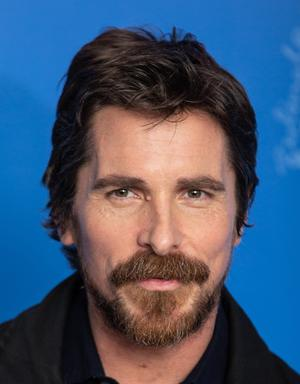
\includegraphics[width=\textwidth]{images/13_m_r.jpg}
    \caption{Occlusion of face due to facial hair.}
    \label{facehair}
  \end{minipage}
  \hfill
    \begin{minipage}{0.32\textwidth}
    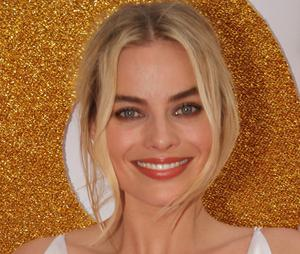
\includegraphics[width=\textwidth]{images/45_f_r.jpg}
    \caption{Expression variation due to smile.}
    \label{facesmile}
  \end{minipage} 
    \hfill
  \begin{minipage}{0.32\textwidth}
    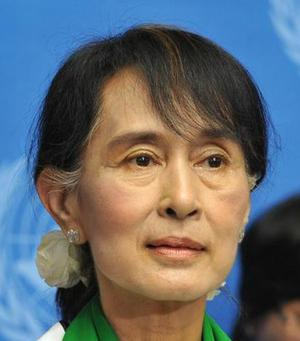
\includegraphics[width=\textwidth]{images/28_f_m.jpg}
    \caption{Pose variation due to head rotation.}
    \label{facepose}
  \end{minipage}
    \hfill
\end{figure}

Considerable effort was put in to the creation of the dataset such that it could provide a valid evaluation for the research into the algorithms bias. This however didn't ensure the dataset was perfect as it had many limitations. The size of the dataset was a major limiting factor. The relatively low number of images meant that the accuracy of the average results would suffer, as well as introduce a larger error margin. The other limitation was the variance present in the characteristics of the images. Images were selected to reduce variance but due to the selection method, it was difficult for every image to be standardised. Variance within the dataset consisted of slight pose variation in which some faces were not fully frontal facing (figure \ref{facepose}) as well as expression (figure \ref{facesmile}), and occlusion due to facial hair (figure \ref{facehair}). These variables of the images were difficult to control and would impact the robustness of the results, when looking for a bias.
%annoation methodloy



%==================================================================================================================================
\chapter{Evaluation}
\label{Evaluation}

This chapter discusses the strategy used to evaluate the algorithms and assess if there exists a bias towards race and gender. It also details the metrics used and the figures generated.
\section{Evaluation Strategy}
The general methodology followed that of previous work such as Gender Shades (\cite{gendershades}) and InclusiveFace (\cite{inclusivenet}). Where an algorithmic framework was chosen and evaluated against a dataset containing an evenly distributed number of faces, of different genders and races. The performance of the algorithm on the different groups indicated if any bias existed towards the groups.

For the specific research question, the algorithms were chosen such that they represented the different aspects of the computer vision field throughout the last 20 years. This was done by using algorithms that had the old foundational hand crafted filter structure, and also using newer state-of-the-art algorithms that leveraged deep learning to detect faces. The dataset used was the 5025 dataset, which consisted of two groups, represented and underrepresned faces, that contained different races and genders. To understand if a bias existed within the range of algorithms, they were executed against the 5025 dataset and the resulting coordinate predictions were compared to the ground truth coordinates for each image. This comparison provided a strong indication to the accuracy of the algorithms against the represented and underrepresented groups. If an algorithm was more accurate for one group over the other, then a bias could exist towards race and gender.
% The euclidean distance between these coordinates was taken, normalised by the distance between the eyes and multiplied by 100. This comparison resulted in "error differences" which showed quantitatively the performance of the algorithm in respect to the represented and underrepresented groups as well as provided a strong means of analysis.
%  The 4 algorithms consisted of concepts such as single shot detection, feature pyramid networks, multi task learning, feature extraction and image pyramids. All of which helped each algorithm distinguish itself such that the 4 algorithms were representative of a wide proportion of the computer vision field
\section{Evaluation Metrics}
\label{experimentaldesign}

The accuracy measure is calculated using the difference between the ground truth coordinates and the algorithms predicted coordinates. This involved taking the euclidean distance between the predetermined ground truth, and the predicted coordinates by the algorithms. This distance value on its own is not useful as a comparison metric because every face differs in size. To combat this discrepancy, each distance value for a face is normalised by the euclidean distance between the ground truth eye landmarks for that face. These normalised values are multiplied by 100 to produce larger numbers to work with. This metric called "Error Differences" is calculated for every annotation across the faces and algorithms. It shows the normalised distance between the ground truth coordinates and the algorithms predicted coordinates for a specified face. 

The metric is used to assess the accuracy of the underrepresented and represented groups in the dataset, and generate the different figures detailed below.
%include image
\subsection{Frequency of Error Differences at Different Thresholds}
The frequency of error difference at different thresholds is calculated by counting the number of error differences above each error difference magnitude for both groups. The number of errors indicates the accuracy of the group. If there is a large number of errors at the large thresholds then the group is inaccurate. The data is plotted as a line graph for both groups, in which a difference between the lines indicates a difference in accuracy.

% The error difference is used to compare and contrast with the two groups of underrepresented and represented faces. By thresholding different magnitudes of difference for every landmark, the number of landmarks which have an error difference value lower than the threshold are recorded between the groups. This shows how accurate each algorithm is, by using its frequency of error differences at every threshold. The data is plotted on a line graph for each group. The graph indicates if there is a difference in the number of errors between underrepresented and represented faces at different magnitudes of error difference. 
\subsection{Bounding Box Accuracy Histogram}
The intersection over union explains a lot about the accuracy of the bounding boxes (\cite{iou}). To calculate this, the area of overlap is divided by the area of union between the ground truth bounding box and predicted bounding box. A high percentage overlap of the predicted bounding box with the ground truth bounding box indicates a high level of accuracy. The percentage of overlap for each face and algorithm is placed into bins with intervals of 4\%. This means that the bins contain the frequencies of certain magnitudes of overlap. Histograms are generated using these bins, which show the distribution of bounding box accuracy between both groups for every algorithm.
\subsection{Landmark Error Difference Histogram}
The landmark error difference histogram gives more detail into the performance of the groups by separating the performance of the algorithm by landmark. To calculate the histogram of error differences for each of the landmarks. The error differences between both groups for each landmark are placed into 7 equally sized bins ranging from 0 to 14 error difference. The bins capture the frequency of the error differences at specific magnitudes for the landmarks. Histograms are generated from the sets of bins for both groups. These histograms show the distribution of error difference for each of landmarks, across both groups and every algorithm. 
% To gain further insight into the specific error differences behind thresholds. Both groups for each of their 5 landmarks had the error differences placed into 7 equally sized bins ranging from 0 to 14 error difference. This captured the frequency of error differences for each of the landmarks in both of the groups and showed the distribution by generating a histogram using these bins.
% To gain further insight each error difference dictionary was split between its underrepresented and represented faces. This was done to get two separate groups. Each landmarks error difference for the both groups was placed into 7 equally sized bins ranging from 0 to 14. This captured the frequencies of error differences and a histogram was created. The histogram showed the distribution of error differences in certain ranges for underrepresented and represented groups. 
\subsection{Average Error Difference}
The average values are calculated by using the landmark error differences of both groups for each of the algorithms. The error differences are added up for every landmark and are divided by the size of the groups, which is 24. This results in average error values for every landmark across the groups and algorithms. Each average value is used to create a difference metric between the groups. This is the average error difference of the underrepresented landmark subtracted by the average error difference of the represented landmark. If the value is positive then represented faces perform better, and if the value is negative then the underrepresented faces perform better. Since the average is being calculated, there is a corresponding uncertainty with it. The uncertainty is calculated through bootstrapping. Where the average results are taken of each landmark for multiple random subsets of the dataset. The standard deviation is calculated of these averages and gives an indication to the uncertainty of the average results for the landmarks.
\subsection{Qualitative Image}
To generate qualitative data each image within the dataset for the HOG, MTCNN and RetinaFace algorithms, has its bounding box and landmark locations imposed onto it. The ground truth is also imposed onto the images, so that visual comparisons can be made between the algorithms and faces. The Viola-Jones algorithm doesn't predict landmarks, so its visualisation only consists of the predicted bounding box and ground truth bounding box imposed onto the images.

\chapter{Results}
\label{results}
This chapter describes the results of the evaluation. The different metrics and figures generated are explained in detail.
\section{Frequency of Error Differences at Different Thresholds}
\label{erroratthresholds}
% The errors at thresholds describe the overall performance of each algorithm by looking at the number of errors above each error threshold, for both groups. 
\begin{figure}[h!]
  \centering
  \begin{minipage}{0.49\textwidth}
    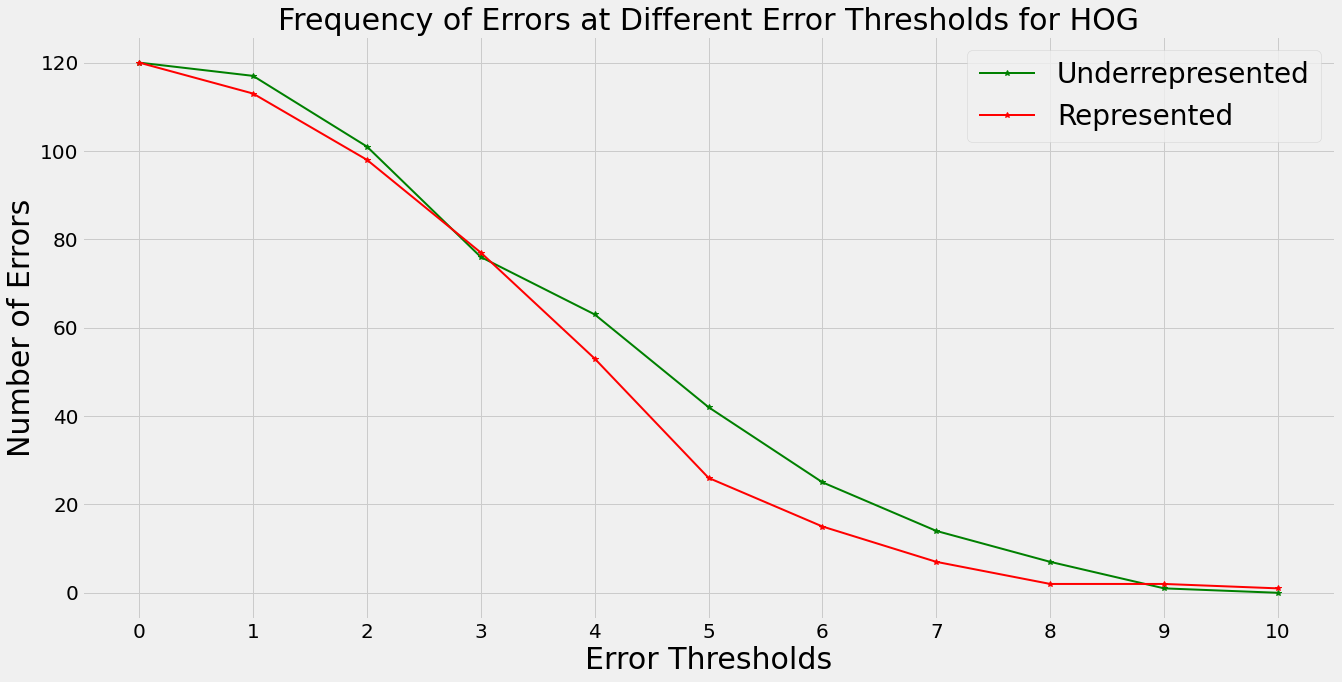
\includegraphics[width=\textwidth]{images/dlib_threshold.png}
    \caption{Threshold graph for HOG error difference.}
    \label{dlib_threshold}
  \end{minipage}
  \hfill
  \begin{minipage}{0.49\textwidth}
    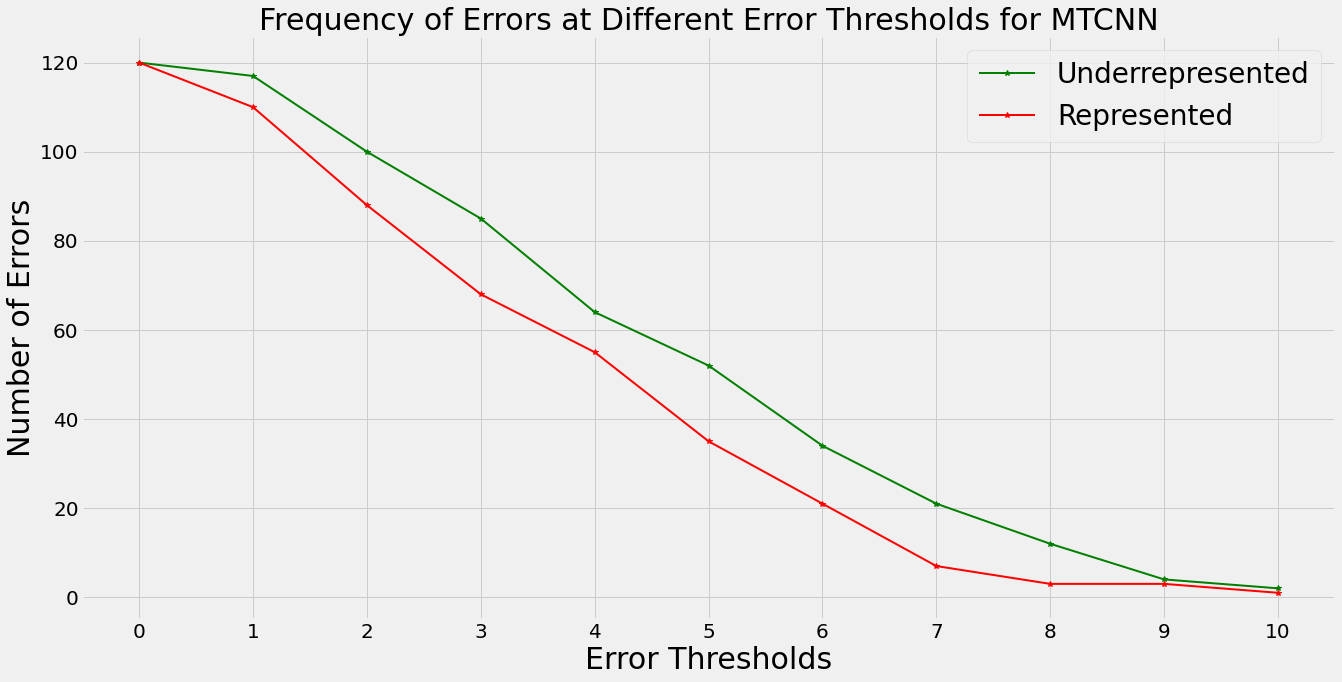
\includegraphics[width=\textwidth]{images/mtcnn_threshold.png}
    \caption{Threshold graph for MTCNN error difference.}
    \label{mtcnn_threshold}
  \end{minipage}
  \hfill
  \begin{minipage}{0.49\textwidth}
    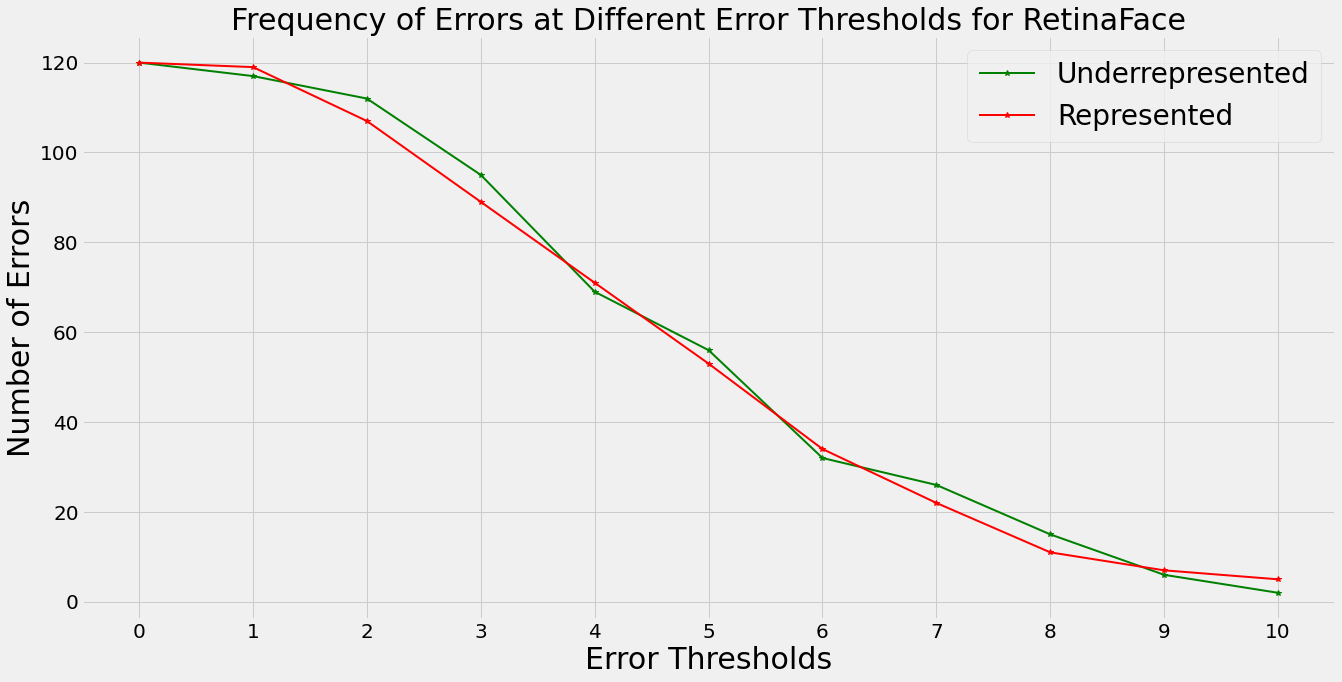
\includegraphics[width=\textwidth]{images/retinaface_threshold.png}
    \caption{Threshold graph for RetinaFace error difference.}
    \label{retinaface_threshold}
  \end{minipage}  
  
\end{figure}

The 3 algorithms exhibit 3 differing trends between the represented and underrepresented groups in the graphs. The HOG algorithm (figure \ref{dlib_threshold}), shows a similar number of errors between the represented and underrepresented groups until the 3 error threshold. However, after this threshold there is consistently more errors for underrepresented faces than there are for represented faces. This differs from the MTCNN algorithm (figure \ref{mtcnn_threshold}), which shows a larger number of errors throughout every error threshold for underrepresented faces, with the largest difference of around 15 errors being between the 5 and 7 thresholds. The RetinaFace algorithm (figure \ref{retinaface_threshold}), performs with more errors in total for each threshold in comparison to the other algorithms, but its performance between represented and underrepresented groups is very similar. With underrepresented faces showing only a slightly higher number of errors at the thresholds.

% The MTCNN algorithm performs worst for underrepresented faces than represented faces. The HOG algorithm follows this to a lesser extent, and the RetinaFace algorithm shows no real disparity between both groups.
\section{Landmark Error Difference Histogram}
% The histograms for each of the algorithms show the same trends that are present in the error thresholds. The histograms are split by landmark, this allows each algorithm to be broken down to see how much a specific facial feature is differing in performance between the groups.
\subsection{HOG}
\begin{figure}[h!]
  \centering
  \begin{minipage}{0.49\textwidth}
    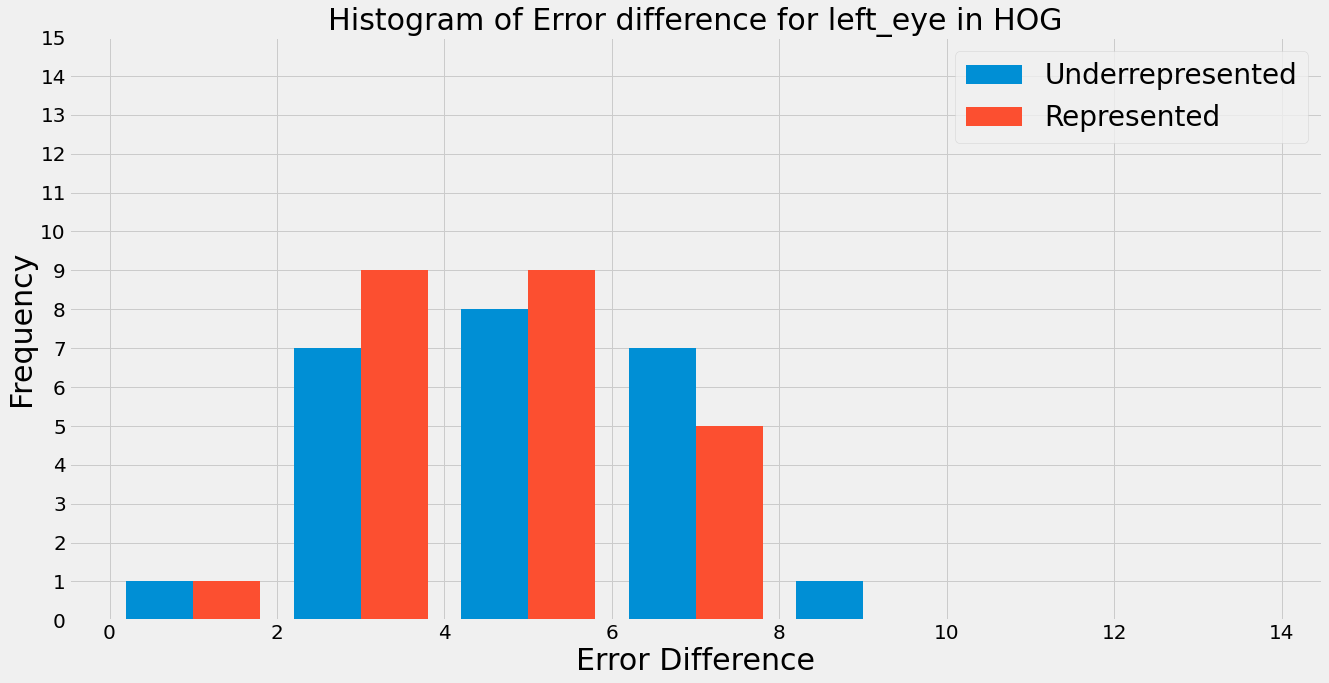
\includegraphics[width=\textwidth]{images/dlib_lefteye.png}
    \caption{Left eye histogram of error difference for HOG.}
    \label{dlib_lefteye}
  \end{minipage}
  \hfill
  \begin{minipage}{0.49\textwidth}
    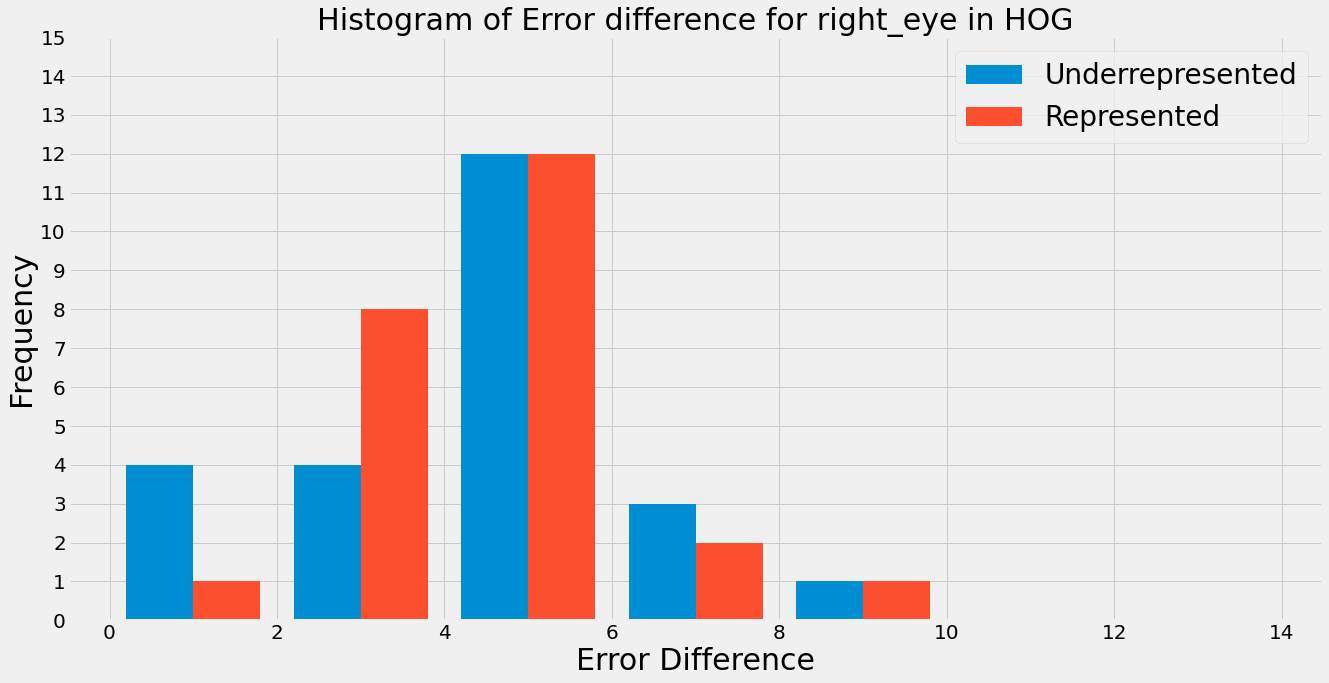
\includegraphics[width=\textwidth]{images/dlib_righteye.png}
    \caption{Right eye histogram of error difference for HOG.}
    \label{dlib_righteye}
  \end{minipage}
  \hfill
  \begin{minipage}{0.51\textwidth}
    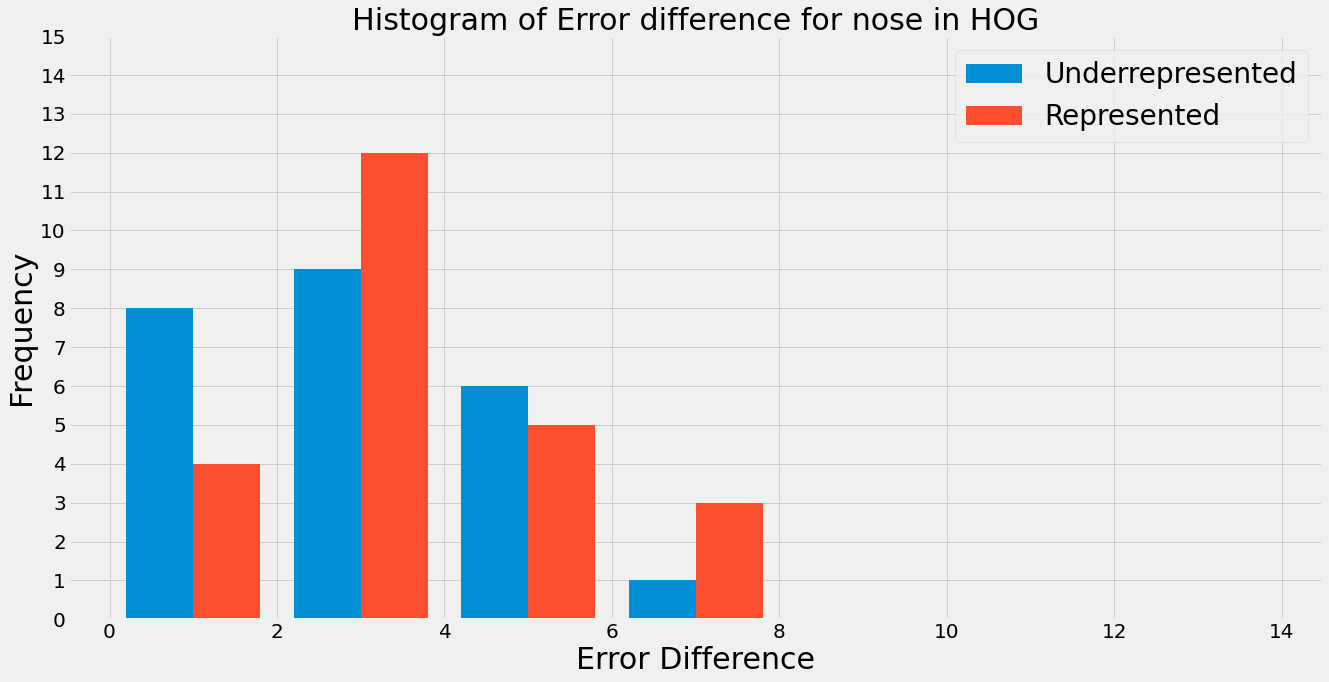
\includegraphics[width=\textwidth]{images/dlib_nose.png}
    \caption{Nose histogram of error difference for HOG.}
    \label{dlib_nose}
  \end{minipage}
    \hfill
  \begin{minipage}{0.49\textwidth}
    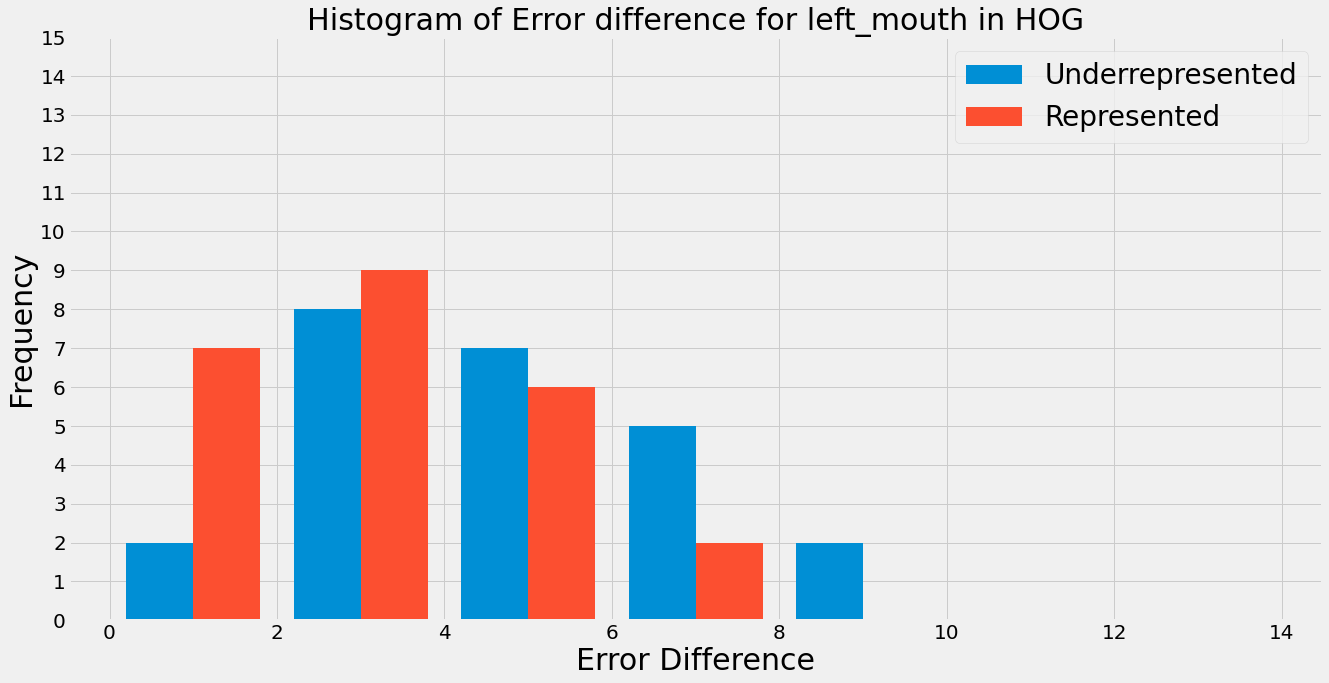
\includegraphics[width=\textwidth]{images/dlib_leftmouth.png}
    \caption{Left mouth histogram of error difference for HOG.}
    \label{dlib_leftmouth}
  \end{minipage} 
      \hfill
    \begin{minipage}{0.49\textwidth}
    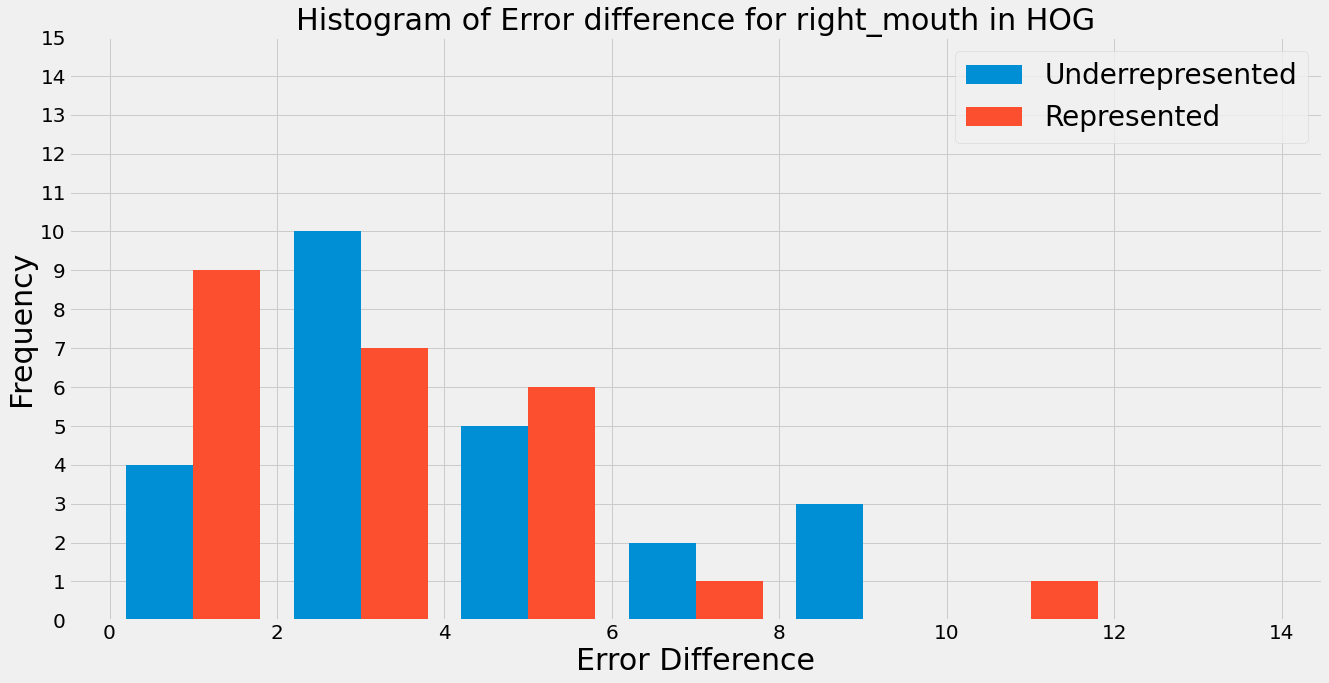
\includegraphics[width=\textwidth]{images/dlib_rightmouth.png}
    \caption{Right mouth histogram of error difference for HOG.}
    \label{dlib_rightmouth}
  \end{minipage} 
 
\end{figure}

Figure \ref{dlib_leftmouth} and figure \ref{dlib_rightmouth} show that the left and right mouth landmark locations for the HOG algorithm have a significant difference between the groups. There are a larger number of errors before the 4 threshold for represented faces than there are for underrepresented faces. This difference being 32 errors in total for the represented group in both landmarks, and 24 for the underrepresented group. For every landmark there is a higher or equal number of errors present for underrepresented faces above the 8 magnitude than there are for represented faces. For both mouth landmarks at the 8 magnitude extreme, there are 5 errors present in total for underrepresented faces and 1 for represented faces. This indicates the underrepresented groups performing worst for the mouth landmarks. Although, for the eye landmarks the difference is of a much smaller magnitude. From figures \ref{dlib_lefteye} and \ref{dlib_righteye}, there are 16 errors in total for left and right eye landmarks of underrepresented faces below the 4 threshold, whereas there are 19 for represented faces. This shows represented faces performing slightly better for the eye landmarks. Looking at figure \ref{dlib_nose}, underrepresented faces perform better than represented for the nose landmark, as there more occurrences of smaller errors for underrepresented faces. This being 8 underrepresented faces under the 2 error threshold, compared to the 4 represented faces. 


\subsection{MTCNN}

\begin{figure}[h!]
  \centering
  \begin{minipage}{0.49\textwidth}
    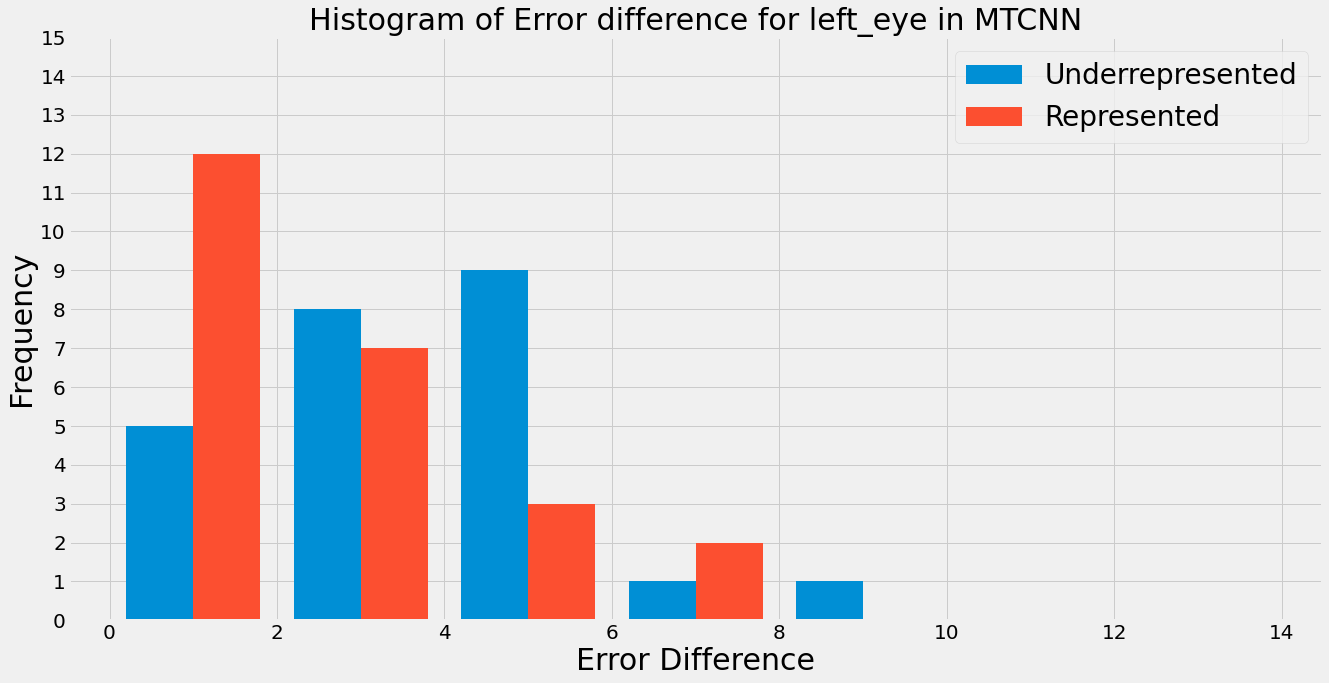
\includegraphics[width=\textwidth]{images/mtcnn_lefteye.png}
    \caption{Left eye histogram of error difference for MTCNN.}
    \label{mtcnn_lefteye}
  \end{minipage}
  \hfill
  \begin{minipage}{0.49\textwidth}
    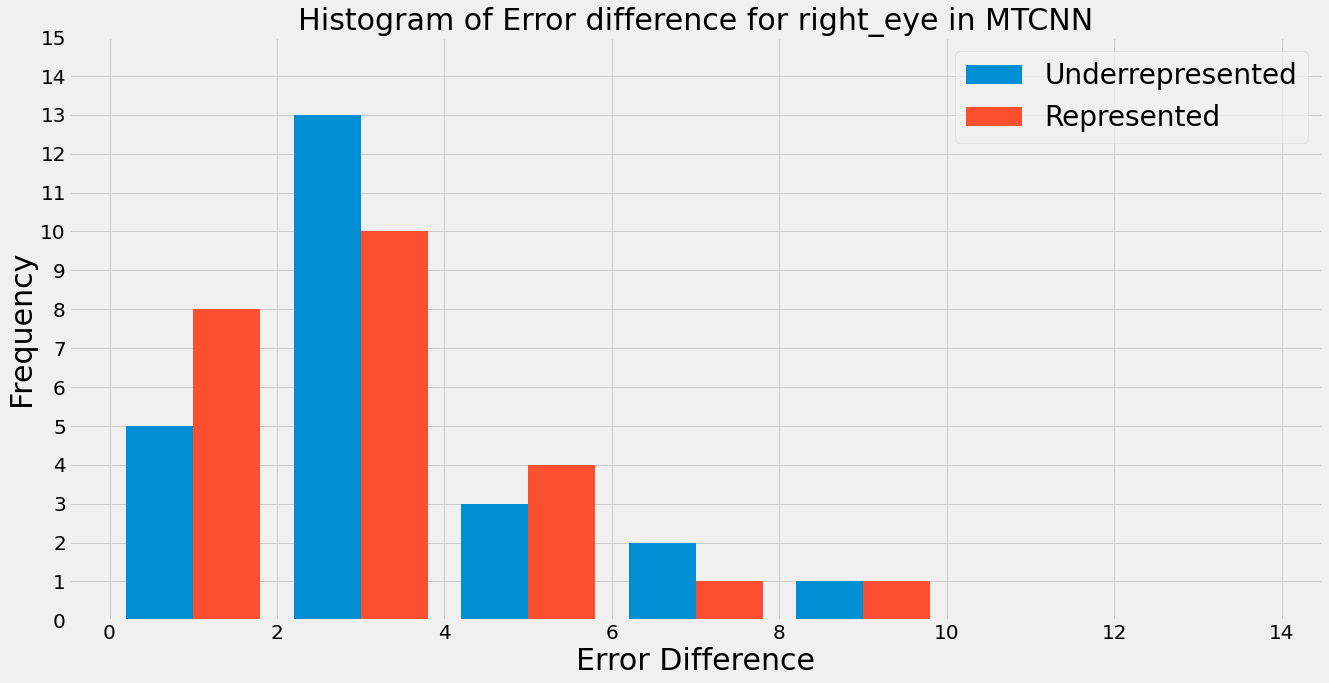
\includegraphics[width=\textwidth]{images/mtcnn_righteye.png}
    \caption{Right eye histogram of error difference for MTCNN.}
    \label{mtcnn_righteye}
  \end{minipage}
  \hfill
  \begin{minipage}{0.51\textwidth}
    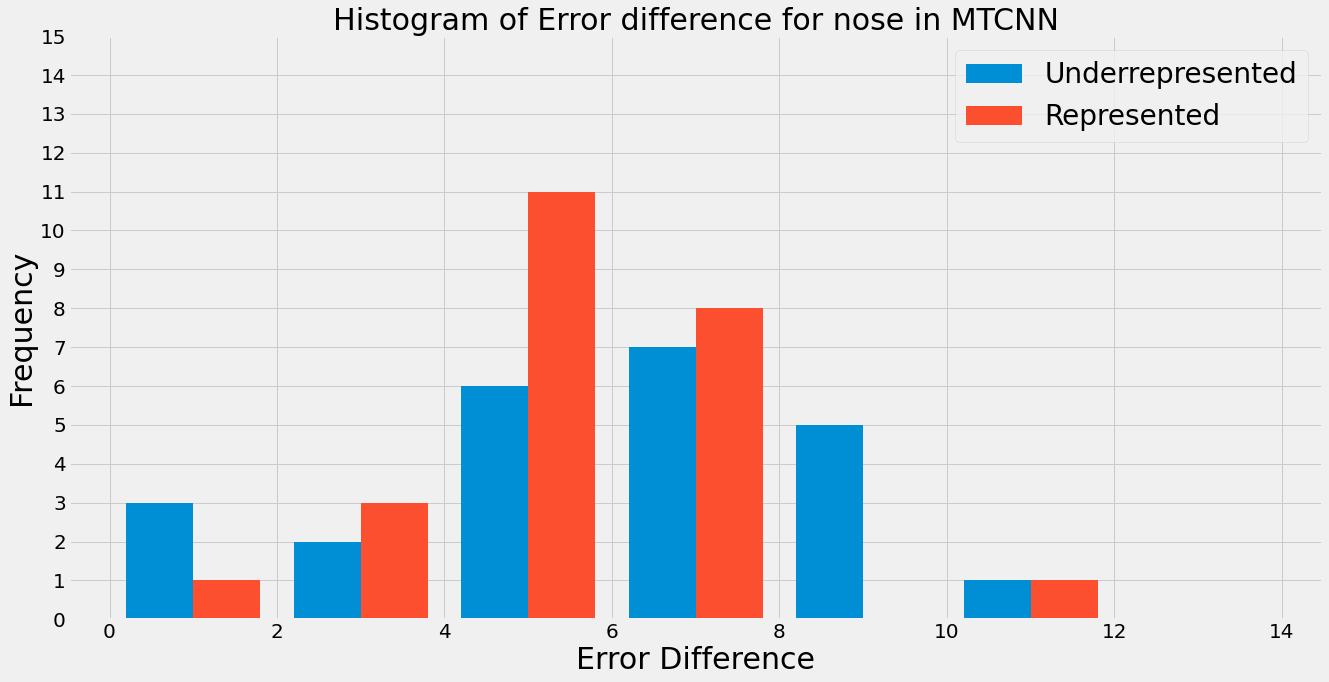
\includegraphics[width=\textwidth]{images/mtcnn_nose.png}
    \caption{Nose histogram of error difference for MTCNN.}
    \label{mtcnn_nose}
  \end{minipage}
    \hfill
  \begin{minipage}{0.49\textwidth}
    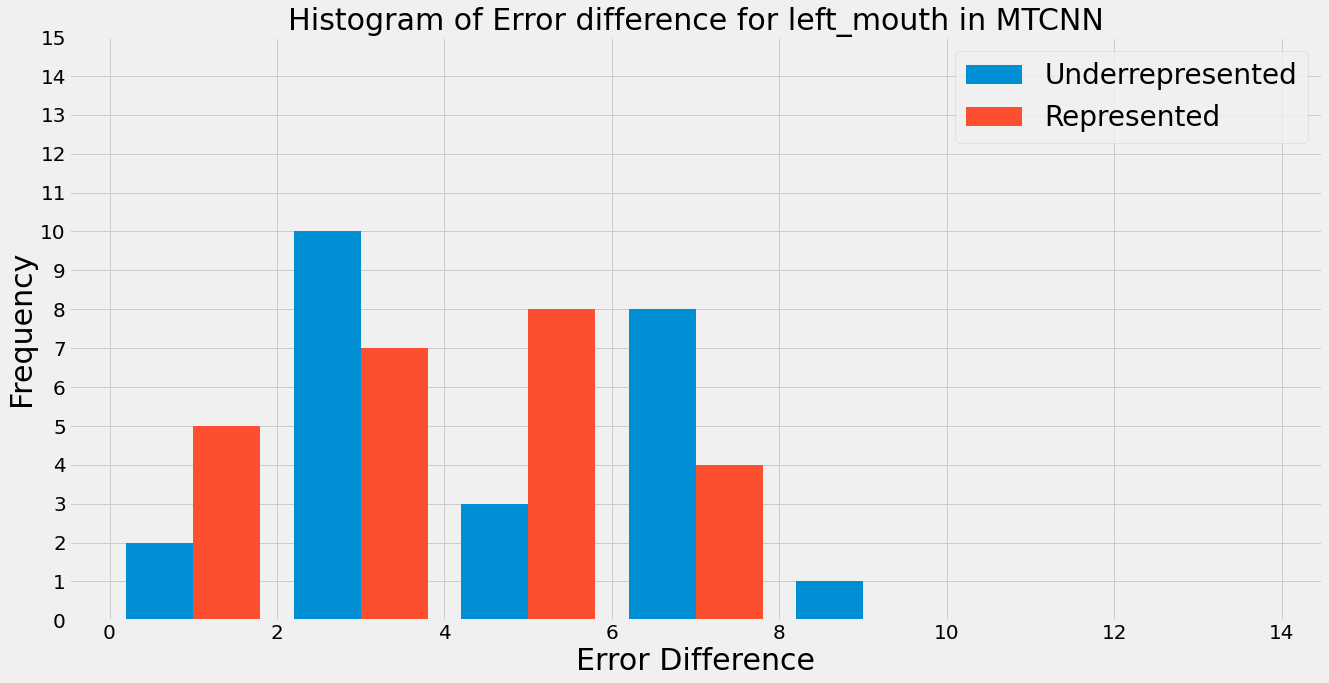
\includegraphics[width=\textwidth]{images/mtcnn_leftmouth.png}
    \caption{Left mouth histogram of error difference for MTCNN.}
    \label{mtcnn_leftmouth}
  \end{minipage} 
      \hfill
    \begin{minipage}{0.49\textwidth}
    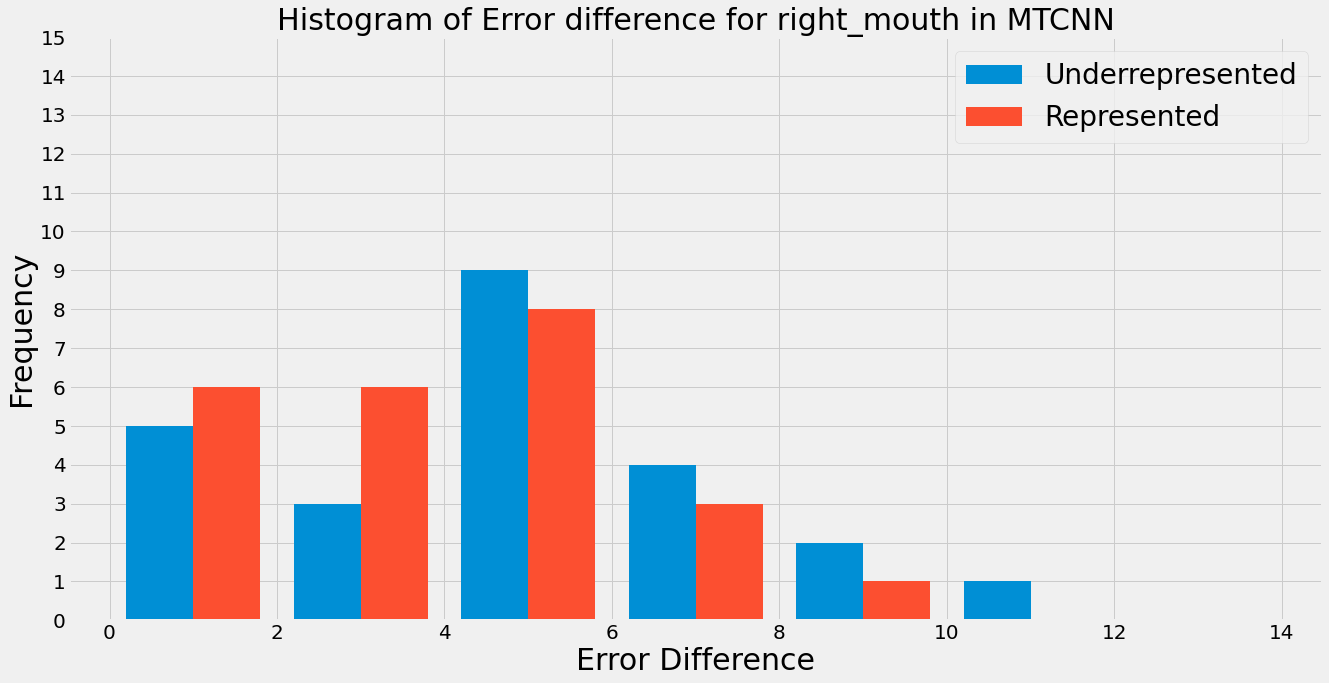
\includegraphics[width=\textwidth]{images/mtcnn_rightmouth.png}
    \caption{Right mouth histogram of error difference for MTCNN.}
    \label{mtcnn_rightmouth}
  \end{minipage} 
 
\end{figure}

The MTCNN algorithm shows that there are more errors that are of a larger magnitude of above 6, for underrepresented faces in each landmark. With the left eye landmark in figure \ref{mtcnn_lefteye}, not being consistent with this result, and instead having an equal number of errors between the groups. The nose landmark (figure \ref{mtcnn_nose}), shows that after the 6 threshold there are 13 errors for underrepresented faces and only 9 for represented faces. However, the majority of the nose errors being 11 out of the possible 24 for represented faces occur between the 4 to 6 error difference magnitudes. This shows that even for represented faces the algorithm isn't entirely accurate. The left mouth (Figure \ref{mtcnn_leftmouth}), shows that under the 2 threshold the represented faces perform better with more errors at smaller magnitude with 5, compared to the 2 for underrepresented faces. Figure \ref{mtcnn_rightmouth} for the right mouth, indicates the represented faces performing better than the underrepresented faces because there are more occurrences of errors at lower thresholds. At the higher thresholds for the mouth landmarks there are more errors for underrepresented faces. The left mouth shows that there are 9 errors above a threshold of 6 for underrepresented faces, where as there are only 4 errors for represented faces. The same can be seen for the right mouth landmark which shows that there are 4 errors for represented faces and 7 for underrepresented faces. This means the mouth landmarks perform much worst for underrepresented faces. The right eye landmark (figure \ref{mtcnn_righteye}), shows that the performance between the groups is very similar but the represented group performs slightly better than the underrepresented. This is seen with there being 8 errors for represented and only 5 for underrepresented faces under the 2 threshold. The left eye landmark (figure \ref{mtcnn_lefteye}), is the only landmark which shows that the represented faces performed equally with the number of errors above the 6 threshold, at 2 errors each. This equal performance is undermined by the higher number of errors for represented faces in the lower thresholds. Below 2 is where most of the represented errors are, with there being 12 errors compared to the 5 errors for underrepresented faces. This shows the represented faces performing better for the left eye landmark. 
% After the 6 threshold for the right eye landmark the difference is even smaller with underrepresented faces having only 1 more error than represented faces
\subsection{RetinaFace}
\begin{figure}[h!]
  \centering
  \begin{minipage}{0.49\textwidth}
    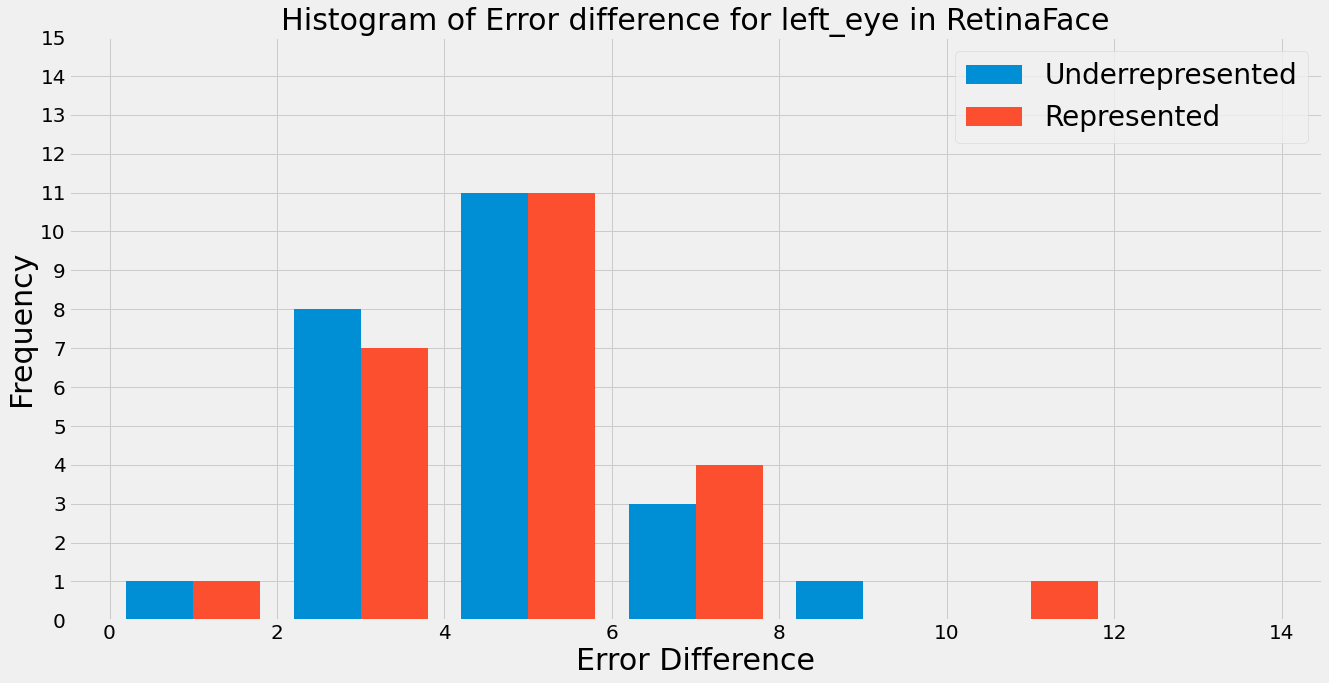
\includegraphics[width=\textwidth]{images/retinaface_lefteye.png}
    \caption{Left eye histogram of error difference for RetinaFace.}
    \label{retinaface_lefteye}
  \end{minipage}
  \hfill
  \begin{minipage}{0.49\textwidth}
    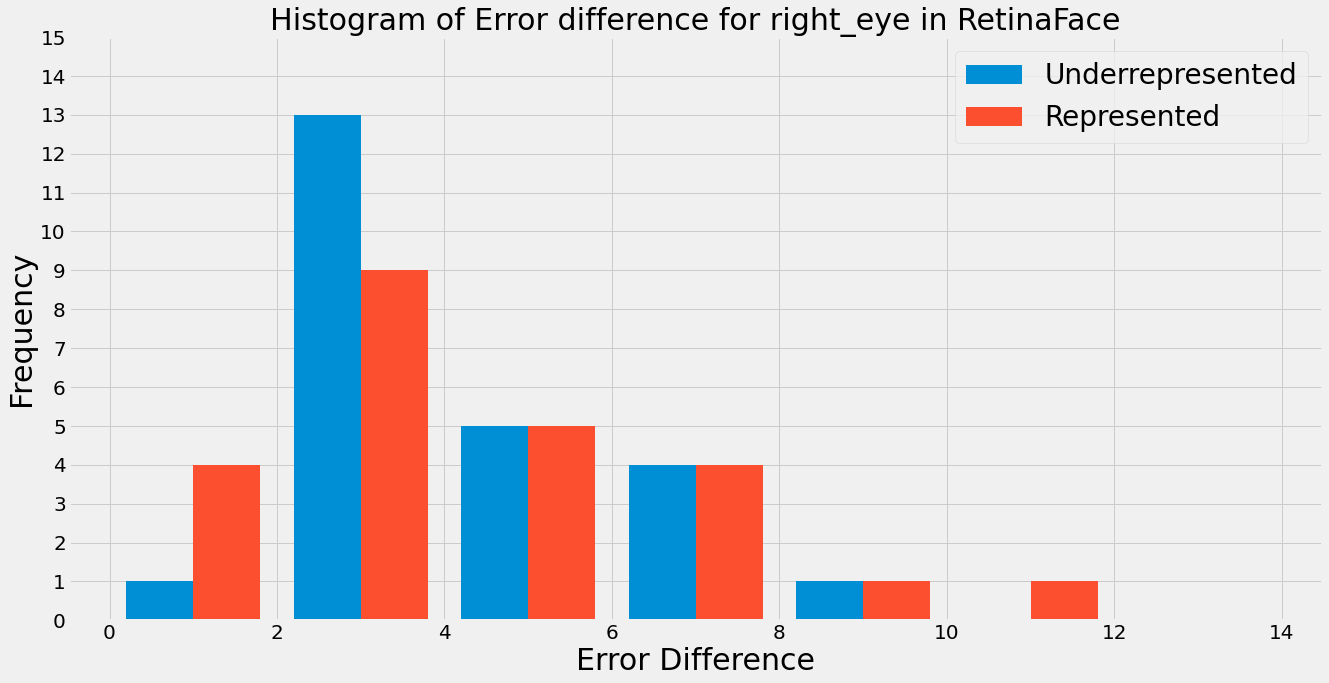
\includegraphics[width=\textwidth]{images/retinaface_righteye.png}
    \caption{Right eye histogram of error difference for RetinaFace.}
    \label{retinaface_righteye}
  \end{minipage}
  \hfill
  \begin{minipage}{0.51\textwidth}
    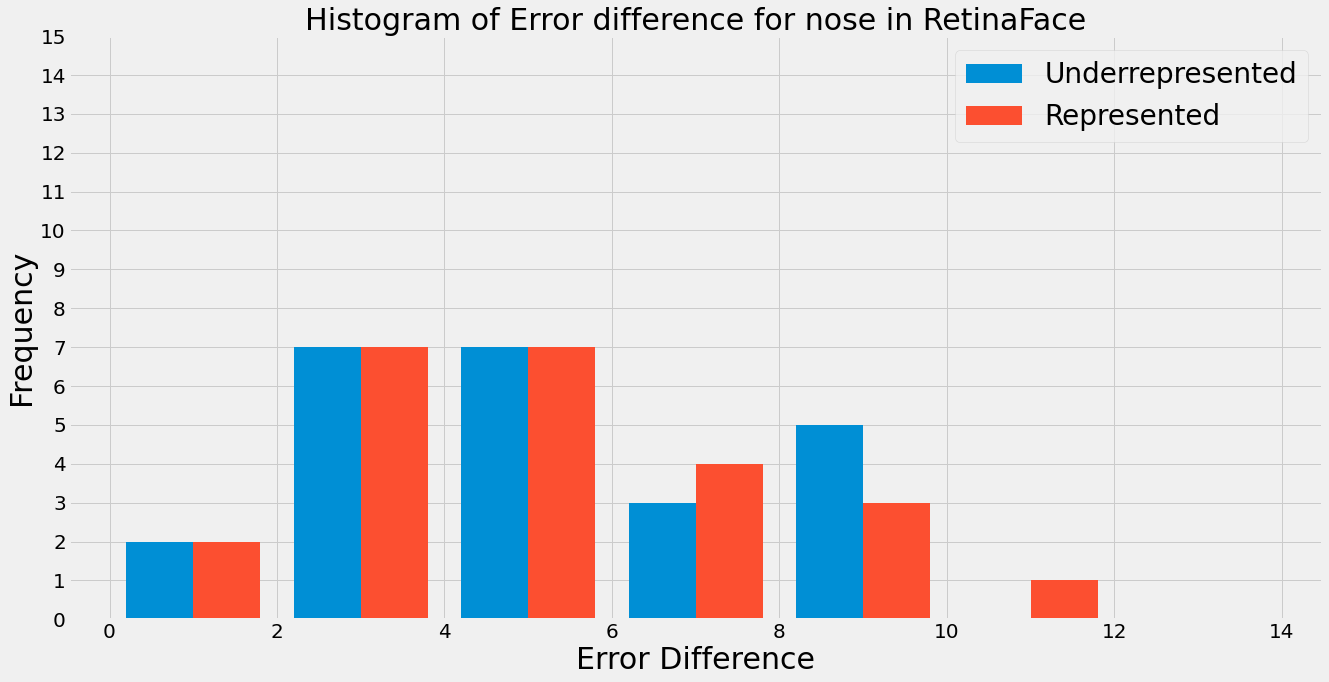
\includegraphics[width=\textwidth]{images/retinaface_nose.png}
    \caption{Nose histogram of error difference for RetinaFace.}
    \label{retinaface_nose}
  \end{minipage}
    \hfill
  \begin{minipage}{0.49\textwidth}
    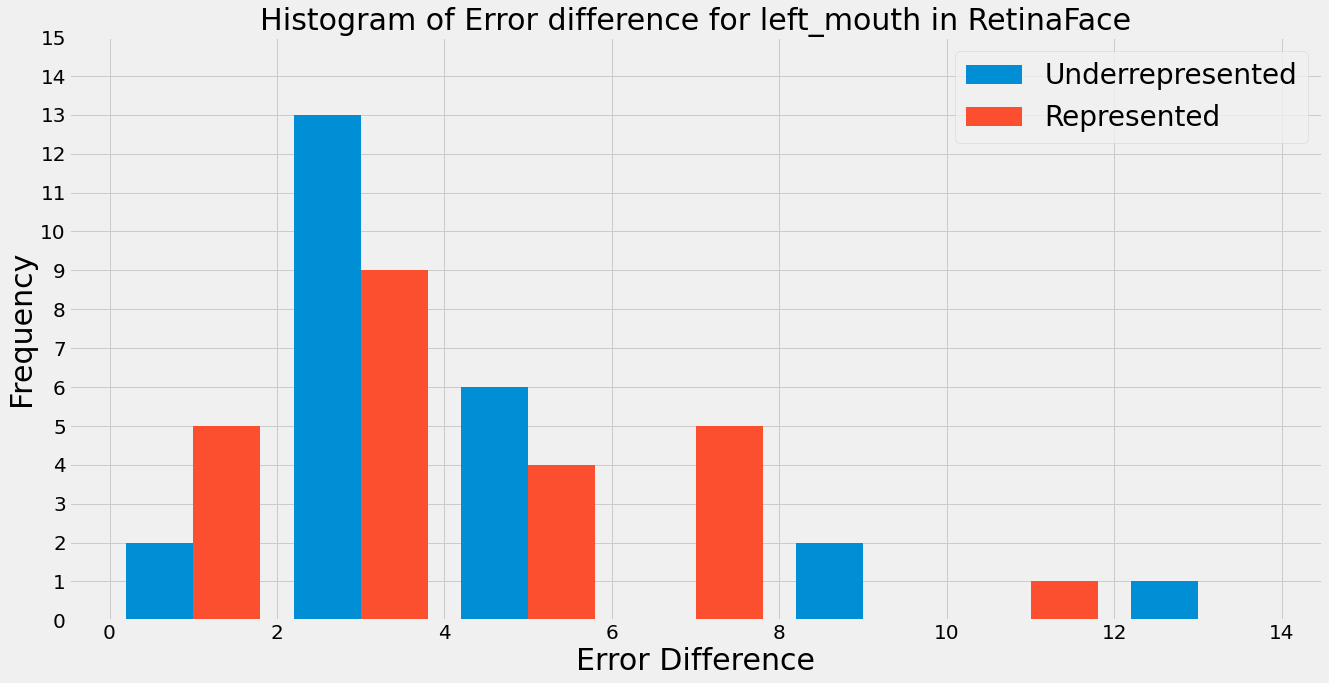
\includegraphics[width=\textwidth]{images/retinaface_leftmouth.png}
    \caption{Left mouth histogram of error difference for RetinaFace.}
    \label{retinaface_leftmouth}
  \end{minipage} 
      \hfill
    \begin{minipage}{0.49\textwidth}
    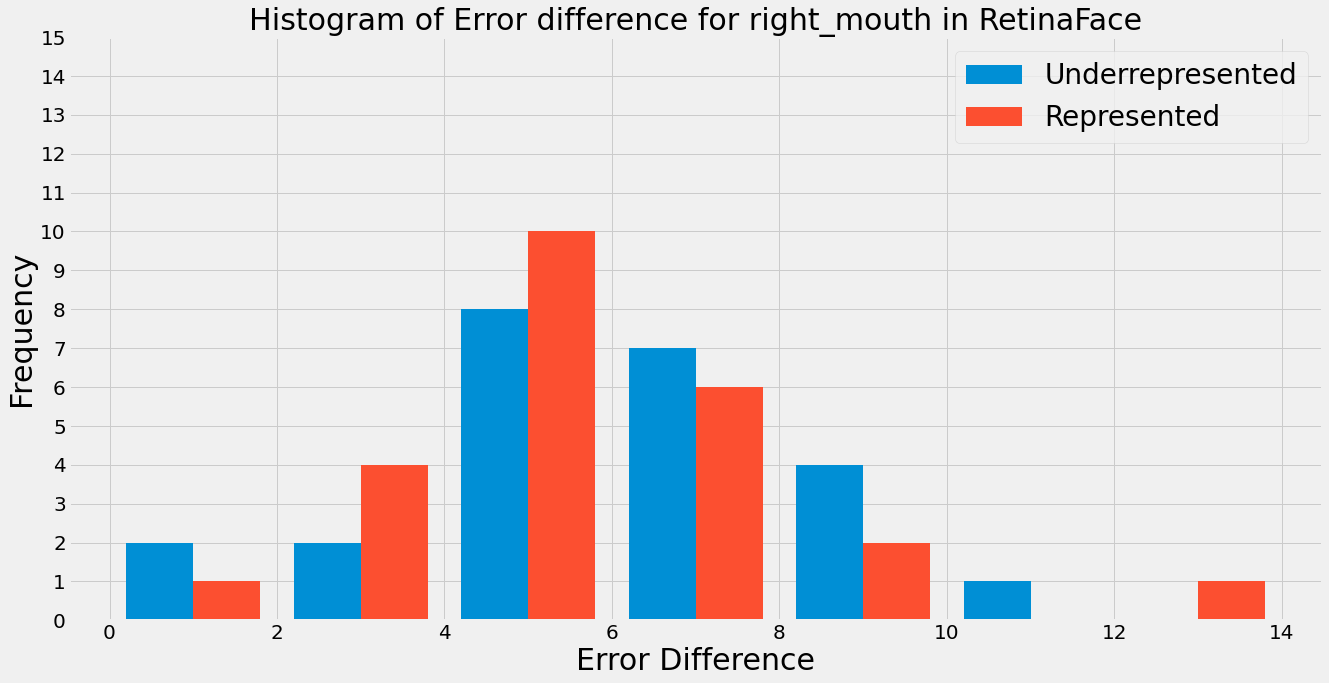
\includegraphics[width=\textwidth]{images/retinaface_rightmouth.png}
    \caption{Right mouth histogram of error difference for RetinaFace.}
    \label{retinaface_rightmouth}
  \end{minipage} 
 
\end{figure}

The RetinaFace algorithm has similar performance between both groups in each of the landmarks. The left mouth landmark (figure \ref{retinaface_leftmouth}), shows the largest difference between the groups under the 4 threshold, with there being 15 errors for underrepresented faces and 13 for represented faces. Figures \ref{retinaface_lefteye} and \ref{retinaface_righteye} for the left eye and right eye both have a difference of 1 error, where there is 1 more error for underrepresented faces. The right mouth landmark seen in figure \ref{retinaface_rightmouth}, also exhibits a difference of 1 error under the 4 threshold, but here there is one more error for represented faces. The nose landmark (figure \ref{retinaface_nose}), shows that under the 4 threshold the number of errors for represented and underrepresented faces are equal at 9 errors. There is no clear difference between the groups in any of the landmarks.
\section{Average Error Difference}

% \begin{figure}[h!]
%   \centering
%   \begin{minipage}{0.48\textwidth}
%     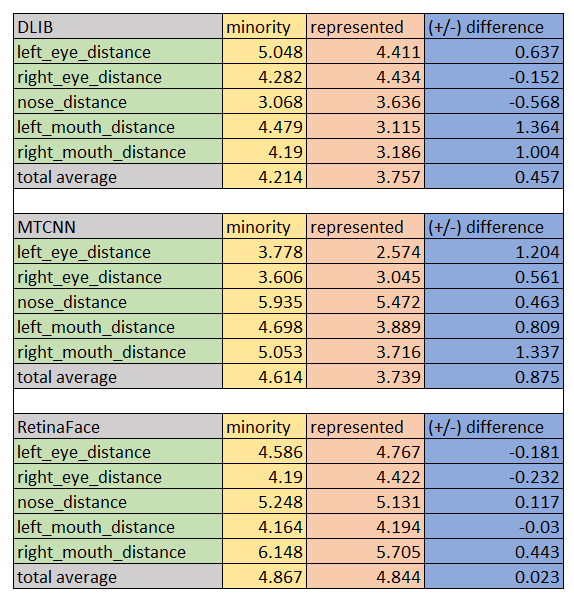
\includegraphics[width=\textwidth]{images/averages.png}
%     \caption{Average Error Values Across Algorithms for Represented and Underrepresented Faces}
%     \label{averages}
%   \end{minipage}
%   \hfill
% \end{figure}
% \begin{table}[!h]
% \centering
% \begin{tabular}{llll}
% \hline
% \multicolumn{1}{|l|}{\textbf{DLIB}} & \multicolumn{1}{l|}{\textbf{minority}} & \multicolumn{1}{l|}{\textbf{represented}} & \multicolumn{1}{l|}{\textbf{(+/-) difference}} \\ \hline
% \multicolumn{1}{|l|}{\textbf{left\_eye\_distance}} & \multicolumn{1}{l|}{5.048} & \multicolumn{1}{l|}{4.411} & \multicolumn{1}{l|}{0.637} \\ \hline
% \multicolumn{1}{|l|}{\textbf{right\_eye\_distance}} & \multicolumn{1}{l|}{4.282} & \multicolumn{1}{l|}{4.434} & \multicolumn{1}{l|}{-0.152} \\ \hline
% \multicolumn{1}{|l|}{\textbf{nose\_distance}} & \multicolumn{1}{l|}{3.068} & \multicolumn{1}{l|}{3.636} & \multicolumn{1}{l|}{-0.568} \\ \hline
% \multicolumn{1}{|l|}{\textbf{left\_mouth\_distance}} & \multicolumn{1}{l|}{4.479} & \multicolumn{1}{l|}{3.115} & \multicolumn{1}{l|}{1.364} \\ \hline
% \multicolumn{1}{|l|}{\textbf{right\_mouth\_distance}} & \multicolumn{1}{l|}{4.19} & \multicolumn{1}{l|}{3.186} & \multicolumn{1}{l|}{1.004} \\ \hline
% \multicolumn{1}{|l|}{\textbf{total average}} & \multicolumn{1}{l|}{4.214} & \multicolumn{1}{l|}{3.757} & \multicolumn{1}{l|}{0.457} \\ \hline
% \textbf{} &  &  &  \\ \hline
% \multicolumn{1}{|l|}{\textbf{MTCNN}} & \multicolumn{1}{l|}{\textbf{minority}} & \multicolumn{1}{l|}{\textbf{represented}} & \multicolumn{1}{l|}{\textbf{(+/-) difference}} \\ \hline
% \multicolumn{1}{|l|}{\textbf{left\_eye\_distance}} & \multicolumn{1}{l|}{3.778} & \multicolumn{1}{l|}{2.574} & \multicolumn{1}{l|}{1.204} \\ \hline
% \multicolumn{1}{|l|}{\textbf{right\_eye\_distance}} & \multicolumn{1}{l|}{3.606} & \multicolumn{1}{l|}{3.045} & \multicolumn{1}{l|}{0.561} \\ \hline
% \multicolumn{1}{|l|}{\textbf{nose\_distance}} & \multicolumn{1}{l|}{5.935} & \multicolumn{1}{l|}{5.472} & \multicolumn{1}{l|}{0.463} \\ \hline
% \multicolumn{1}{|l|}{\textbf{left\_mouth\_distance}} & \multicolumn{1}{l|}{4.698} & \multicolumn{1}{l|}{3.889} & \multicolumn{1}{l|}{0.809} \\ \hline
% \multicolumn{1}{|l|}{\textbf{right\_mouth\_distance}} & \multicolumn{1}{l|}{5.053} & \multicolumn{1}{l|}{3.716} & \multicolumn{1}{l|}{1.337} \\ \hline
% \multicolumn{1}{|l|}{\textbf{total average}} & \multicolumn{1}{l|}{4.614} & \multicolumn{1}{l|}{3.739} & \multicolumn{1}{l|}{0.875} \\ \hline
% \textbf{} &  &  &  \\ \hline
% \multicolumn{1}{|l|}{\textbf{RetinaFace}} & \multicolumn{1}{l|}{\textbf{minority}} & \multicolumn{1}{l|}{\textbf{represented}} & \multicolumn{1}{l|}{\textbf{(+/-) difference}} \\ \hline
% \multicolumn{1}{|l|}{\textbf{left\_eye\_distance}} & \multicolumn{1}{l|}{4.586} & \multicolumn{1}{l|}{4.767} & \multicolumn{1}{l|}{-0.181} \\ \hline
% \multicolumn{1}{|l|}{\textbf{right\_eye\_distance}} & \multicolumn{1}{l|}{4.19} & \multicolumn{1}{l|}{4.422} & \multicolumn{1}{l|}{-0.232} \\ \hline
% \multicolumn{1}{|l|}{\textbf{nose\_distance}} & \multicolumn{1}{l|}{5.248} & \multicolumn{1}{l|}{5.131} & \multicolumn{1}{l|}{0.117} \\ \hline
% \multicolumn{1}{|l|}{\textbf{left\_mouth\_distance}} & \multicolumn{1}{l|}{4.164} & \multicolumn{1}{l|}{4.194} & \multicolumn{1}{l|}{-0.03} \\ \hline
% \multicolumn{1}{|l|}{\textbf{right\_mouth\_distance}} & \multicolumn{1}{l|}{6.148} & \multicolumn{1}{l|}{5.705} & \multicolumn{1}{l|}{0.443} \\ \hline
% \multicolumn{1}{|l|}{\textbf{total average}} & \multicolumn{1}{l|}{4.867} & \multicolumn{1}{l|}{4.844} & \multicolumn{1}{l|}{0.023} \\ \hline
% \end{tabular}
% \vspace*{3mm}
% \caption{Average Error Values Across Algorithms for Represented and Underrepresented Faces}
% \label{averages}
% \end{table}
\begin{table}[h!]
\begin{tabular}{lllll}
\hline
\multicolumn{1}{|l|}{\textbf{HOG}} & \multicolumn{1}{l|}{\textbf{Underrepresented}} & \multicolumn{1}{l|}{\textbf{Represented}} & \multicolumn{1}{l|}{\textbf{Uncertainty (+/-)}} & \multicolumn{1}{l|}{\textbf{Difference}} \\ \hline
\multicolumn{1}{|l|}{left\_eye\_distance} & \multicolumn{1}{l|}{5.048} & \multicolumn{1}{l|}{4.411} & \multicolumn{1}{l|}{0.246} & \multicolumn{1}{l|}{\textbf{0.637}} \\ \hline
\multicolumn{1}{|l|}{right\_eye\_distance} & \multicolumn{1}{l|}{4.282} & \multicolumn{1}{l|}{4.434} & \multicolumn{1}{l|}{0.131} & \multicolumn{1}{l|}{-0.152} \\ \hline
\multicolumn{1}{|l|}{nose\_distance} & \multicolumn{1}{l|}{3.068} & \multicolumn{1}{l|}{3.636} & \multicolumn{1}{l|}{0.151} & \multicolumn{1}{l|}{-0.568} \\ \hline
\multicolumn{1}{|l|}{left\_mouth\_distance} & \multicolumn{1}{l|}{4.479} & \multicolumn{1}{l|}{3.115} & \multicolumn{1}{l|}{0.093} & \multicolumn{1}{l|}{\textbf{1.364}} \\ \hline
\multicolumn{1}{|l|}{right\_mouth\_distance} & \multicolumn{1}{l|}{4.19} & \multicolumn{1}{l|}{3.186} & \multicolumn{1}{l|}{0.436} & \multicolumn{1}{l|}{\textbf{1.004}} \\ \hline
\multicolumn{1}{|l|}{total average} & \multicolumn{1}{l|}{4.214} & \multicolumn{1}{l|}{3.757} & \multicolumn{1}{l|}{0.547} & \multicolumn{1}{l|}{\textbf{0.457}} \\ \hline
 &  &  &  &  \\ \hline
\multicolumn{1}{|l|}{\textbf{MTCNN}} & \multicolumn{1}{l|}{\textbf{Underrepresented}} & \multicolumn{1}{l|}{\textbf{Represented}} & \multicolumn{1}{l|}{\textbf{Uncertainty (+/-)}} & \multicolumn{1}{l|}{\textbf{Difference}} \\ \hline
\multicolumn{1}{|l|}{left\_eye\_distance} & \multicolumn{1}{l|}{3.778} & \multicolumn{1}{l|}{2.574} & \multicolumn{1}{l|}{0.196} & \multicolumn{1}{l|}{\textbf{1.204}} \\ \hline
\multicolumn{1}{|l|}{right\_eye\_distance} & \multicolumn{1}{l|}{3.606} & \multicolumn{1}{l|}{3.045} & \multicolumn{1}{l|}{0.132} & \multicolumn{1}{l|}{\textbf{0.561}} \\ \hline
\multicolumn{1}{|l|}{nose\_distance} & \multicolumn{1}{l|}{5.935} & \multicolumn{1}{l|}{5.472} & \multicolumn{1}{l|}{0.392} & \multicolumn{1}{l|}{\textbf{0.463}} \\ \hline
\multicolumn{1}{|l|}{left\_mouth\_distance} & \multicolumn{1}{l|}{4.698} & \multicolumn{1}{l|}{3.889} & \multicolumn{1}{l|}{0.249} & \multicolumn{1}{l|}{\textbf{0.809}} \\ \hline
\multicolumn{1}{|l|}{right\_mouth\_distance} & \multicolumn{1}{l|}{5.053} & \multicolumn{1}{l|}{3.716} & \multicolumn{1}{l|}{0.42} & \multicolumn{1}{l|}{\textbf{1.337}} \\ \hline
\multicolumn{1}{|l|}{total average} & \multicolumn{1}{l|}{4.614} & \multicolumn{1}{l|}{3.739} & \multicolumn{1}{l|}{0.669} & \multicolumn{1}{l|}{\textbf{0.875}} \\ \hline
 &  &  &  &  \\ \hline
\multicolumn{1}{|l|}{\textbf{RetinaFace}} & \multicolumn{1}{l|}{\textbf{Underrepresented}} & \multicolumn{1}{l|}{\textbf{Represented}} & \multicolumn{1}{l|}{\textbf{Uncertainty (+/-)}} & \multicolumn{1}{l|}{\textbf{Difference}} \\ \hline
\multicolumn{1}{|l|}{left\_eye\_distance} & \multicolumn{1}{l|}{4.586} & \multicolumn{1}{l|}{4.767} & \multicolumn{1}{l|}{0.181} & \multicolumn{1}{l|}{-0.181} \\ \hline
\multicolumn{1}{|l|}{right\_eye\_distance} & \multicolumn{1}{l|}{4.19} & \multicolumn{1}{l|}{4.422} & \multicolumn{1}{l|}{0.311} & \multicolumn{1}{l|}{-0.232} \\ \hline
\multicolumn{1}{|l|}{nose\_distance} & \multicolumn{1}{l|}{5.248} & \multicolumn{1}{l|}{5.131} & \multicolumn{1}{l|}{0.415} & \multicolumn{1}{l|}{\textbf{0.117}} \\ \hline
\multicolumn{1}{|l|}{left\_mouth\_distance} & \multicolumn{1}{l|}{4.164} & \multicolumn{1}{l|}{4.194} & \multicolumn{1}{l|}{0.319} & \multicolumn{1}{l|}{-0.03} \\ \hline
\multicolumn{1}{|l|}{right\_mouth\_distance} & \multicolumn{1}{l|}{6.148} & \multicolumn{1}{l|}{5.705} & \multicolumn{1}{l|}{0.344} & \multicolumn{1}{l|}{\textbf{0.443}} \\ \hline
\multicolumn{1}{|l|}{total average} & \multicolumn{1}{l|}{4.867} & \multicolumn{1}{l|}{4.844} & \multicolumn{1}{l|}{0.722} & \multicolumn{1}{l|}{\textbf{0.023}} \\ \hline
\end{tabular}
\vspace*{3mm}
\caption{Average error values across algorithms for represented and underrepresented faces.}
\label{averages}
\end{table}
% \vspace*{3mm}
% \caption{Average Error Values Across Algorithms for Represented and Underrepresented Faces}
% \label{averages}
The average difference values from table \ref{averages}, described how much each algorithms performance leaned in relation to underrepresented or represented faces. The average values provided a metric that could be compared across both landmarks and algorithms for the entire dataset. The uncertainty values were calculated through bootstrapping by using the standard deviation of averages for multiple subsets of the results.
\subsection{HOG}
The largest average error difference for the HOG algorithm was at the left mouth landmark with a difference of 1.364. This difference was towards underrepresented faces being more inaccurate. The right mouth and left eye landmarks showed similar results but of a smaller magnitude, with right mouth having a difference of 1.004 and left eye with 0.637. It is important to point out that the left eye had the largest overall average error at 5.048 for underrepresented faces and was the worst performing landmark for the HOG algorithm. The right eye and nose landmark showed differences leaning towards the represented faces performing worst. The right eye had a difference of -0.152 and the nose had a difference of -0.568. Overall the performance of the nose landmark was the most accurate for represented and underrepresented faces for the HOG algorithm. The average of all the landmarks in the represented faces was 3.757, with the average of underrepresented faces being 4.214, giving a difference of 0.457 towards underrepresented faces performing worst. 
\subsection{MTCNN}
The MTCNN algorithm overall performed worst for underrepresented faces than it did for represented faces. All the landmarks have an average difference that is towards underrepresented faces performing worst, with the largest difference being the right mouth landmark. The right mouth landmark shows a difference of 1.337 between the represented and underrepresented averages. The left eye landmark also has a large difference between the averages of the two groups at 1.204. The nose landmark is the worst performing landmark in terms of averages for both of the groups, with an average of 5.935 for underrepresented faces and 5.472 for represented faces. Even though this landmark has the worst performance, it has the smallest difference between the two groups at 0.463. The left mouth landmark and right eye landmark show results consistent with the other landmarks, with differences of 0.809 and 0.561 respectively. The average for all the landmarks of represented faces is 3.739 whereas the average for underrepresented faces is 4.614 which gives a large difference of 0.875. This overall shows the underrepresented group performing worst than the represented.
\subsection{RetinaFace}
The RetinaFace algorithm has little difference between the represented and underrepresented faces. The largest difference is present in the right mouth landmark, for which the average error is 6.148 for underrepresented faces and 5.705 for represented faces, giving a 0.443 difference. The left mouth landmark shows the smallest difference between the groups at -0.03, this is also the smallest average difference in all of the algorithms. The right mouth landmark shows the largest difference between the groups at 0.438, where underrepresented faces perform worst. The right mouth landmark is also overall the worst performing landmark for both groups, with the right mouth for underrepresented faces having the worst average performance throughout all the algorithms at 6.148. The left and right eye landmarks both have slightly higher averages for the represented faces giving them a difference of -0.181 and -0.232 respectively. The nose landmark is the only other landmark besides the right mouth landmark where the underrepresented group performs worst than the represented group. Here the difference leans towards the underrepresented group performing worst but is still of a small magnitude at 0.117. The average error of all the landmarks is 4.867 for underrepresented faces and 4.844 for represented faces. This gives a small difference of 0.023 for the algorithm, which shows it performance is very similar between both groups across the landmarks. 

\section{Bounding Box Accuracy Histogram}
Besides landmarks the algorithms also produced bounding boxes around faces that they detected. Looking at the overlap with the ground truth was a strong indication of the accuracy.
\begin{figure}[h!]
  \centering
  \begin{minipage}{0.49\textwidth}
    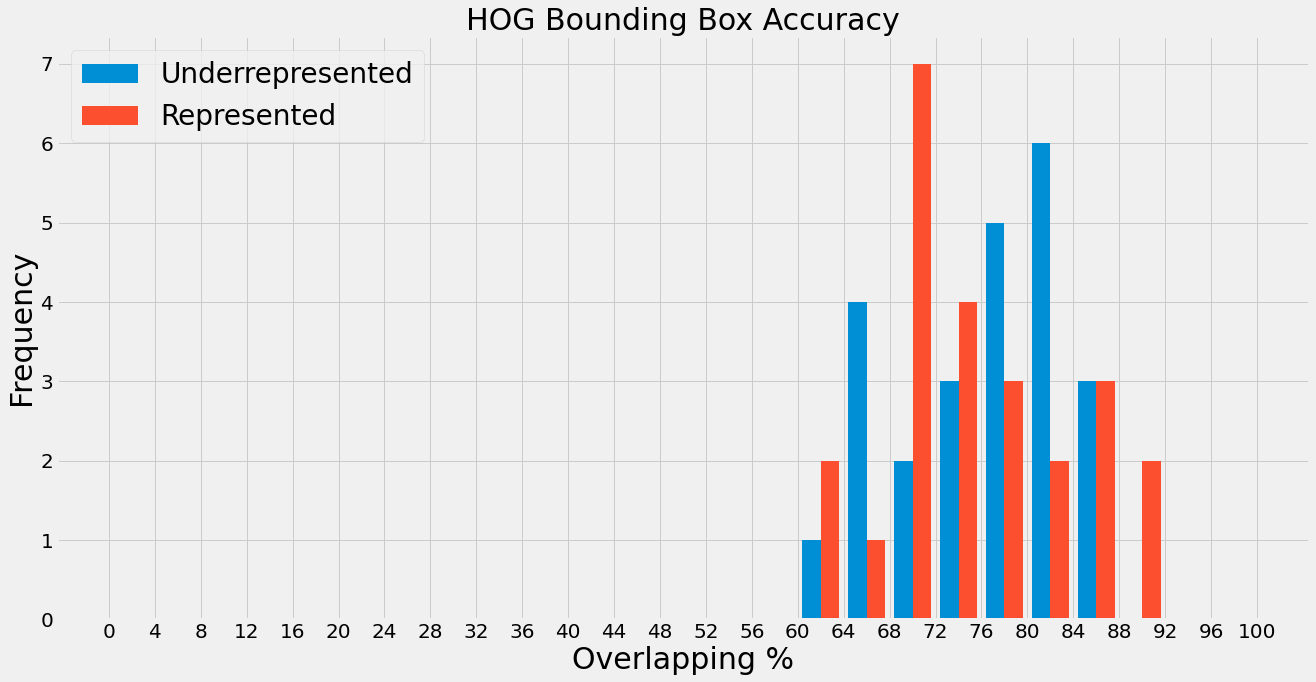
\includegraphics[width=\textwidth]{images/dlib_box.png}
    \caption{Bounding box accuracy histogram for HOG.}
    \label{dlib_box}
  \end{minipage}
  \hfill
  \begin{minipage}{0.49\textwidth}
    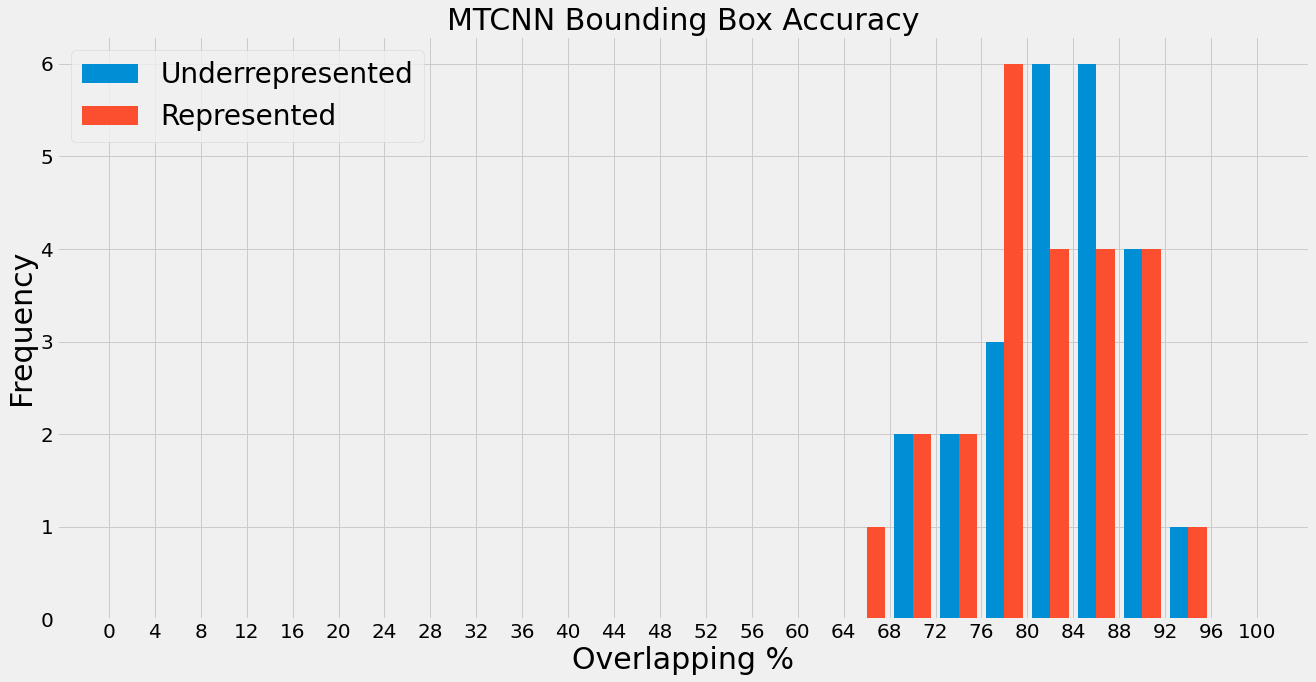
\includegraphics[width=\textwidth]{images/mtcnn_box.png}
    \caption{Bounding box accuracy histogram for MTCNN.}
    \label{mtcnn_box}
  \end{minipage}
  \hfill
  \begin{minipage}{0.49\textwidth}
    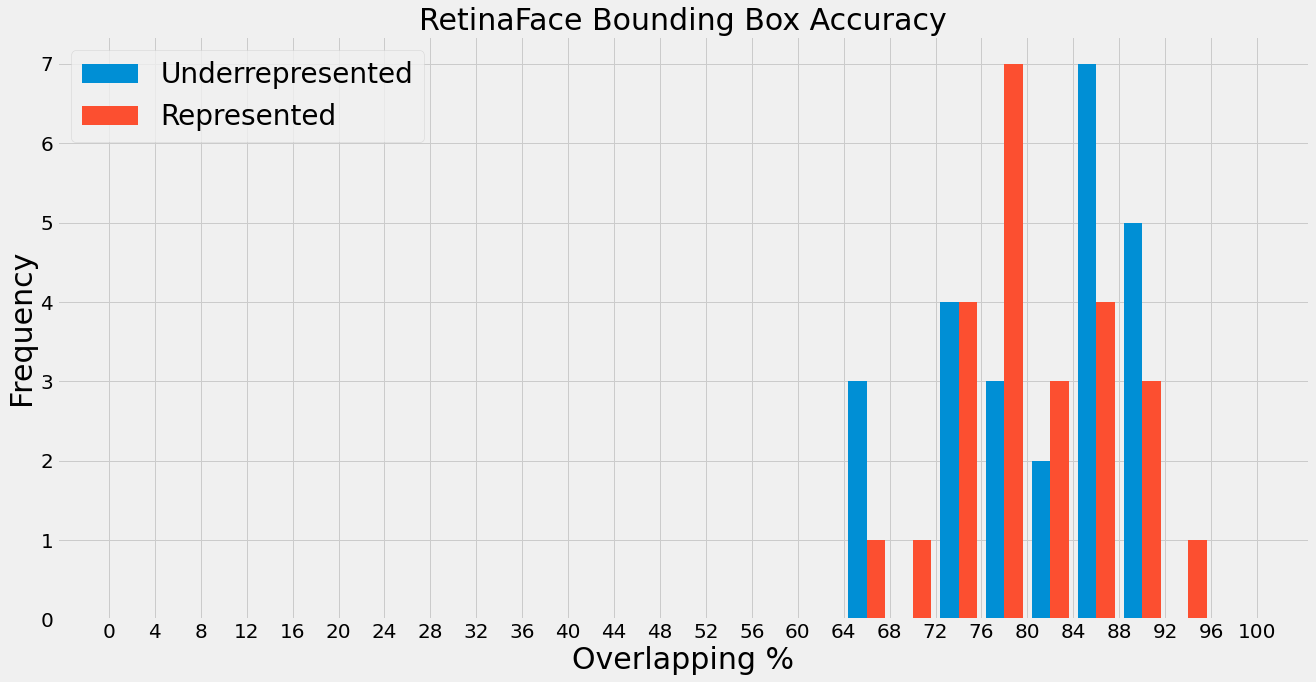
\includegraphics[width=\textwidth]{images/retinaface_box.png}
    \caption{Bounding box accuracy histogram for RetinaFace.}
    \label{retinaface_box}
  \end{minipage}
    \hfill
  \begin{minipage}{0.49\textwidth}
    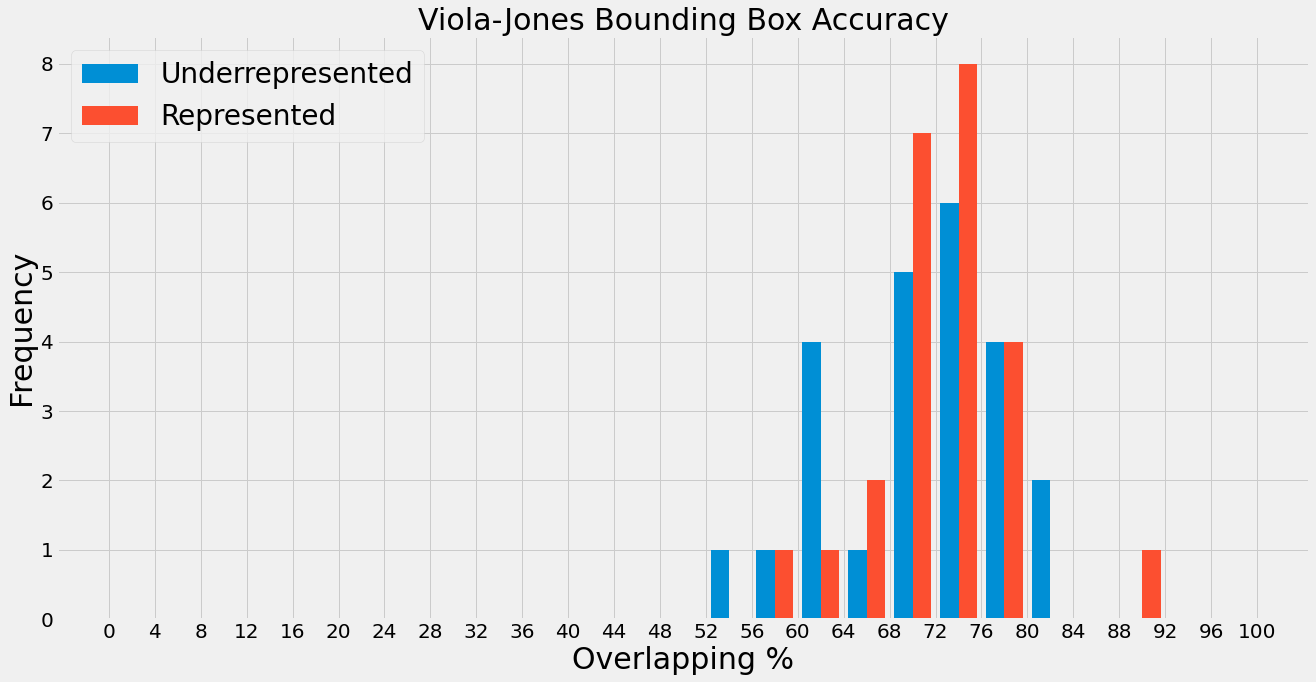
\includegraphics[width=\textwidth]{images/viola_box.png}
    \caption{Bounding box accuracy histogram for Viola-Jones.}
    \label{viola_box}
  \end{minipage} 
 
\end{figure}

For the HOG algorithm in figure \ref{dlib_box}, it is evident that majority of represented faces are between 68\% and 76\%, with the majority of underrepresented faces between 76\% to 80\%. However, in the lowest percentages from 60\% to 68\% there are 5 underrepresented faces and 3 represented faces. At the other end of the spectrum above 88\% there are no underrepresented faces but 2 represented faces. This shows that at the extremes, underrepresented faces perform worst. MTCNN shows that in figure \ref{mtcnn_box}, the bounding box overlap of both groups is very high in the percentages and very similar. There is the same amount of faces with an accuracy above 88\% for both groups. The difference is present between the 76\% to 88\% window, where represented faces perform slightly worst than underrepresented faces. Although overall the performance is very good for both groups. RetinaFace (figure \ref{retinaface_box}), shows underrepresented faces performing better as there are 12 faces present above 84\%, whereas there are only 8 for the represented group. Overall the performance for both groups is similar, with represented faces performing slightly worst. The Viola-Jones algorithm seen in figure \ref{viola_box}, shows that the algorithm performs worst for underrepresented faces as there are 6 underrepresented faces under 64\%, whereas there are only 2 represented faces. The majority of represented faces are in the accurate bounds of 68\% to 80\%, with their being 19 represented faces present in comparison to the 15 underrepresented faces.


%==================================================================================================================================
\chapter{Discussion}
This chapter contains the analysis of the results from the evaluations. They are explained with respect to the research question of the project to understand if, and why there exists a bias towards race and gender. 
\section{Viola-Jones}
This algorithm performs the worst in regards to its bounding boxes between both groups, although in its lowest percentages, there is a distinctly larger number of underrepresented faces than represented. This difference in performance could come from the fact that the the algorithm is an old foundational method. Its filter was created manually through the use of specific haar-like features. This feature representation is the core of the algorithm and is where the slight bias observed could be introduced. The haar-like features work by looking at the difference in regions of pixel intensity in the image. This helps the algorithm classify what features are being observed and if a face is detected. By using the difference in pixel intensities, the algorithm is looking directly at the difference in regions of brightness in an image. In represented faces of a lighter skin tone, this difference in brightness could be exaggerated and be easier for the classifier to understand. Whereas, in underrepresented darker skin toned faces, the difference between areas of intensity could be harder for the algorithm to distinguish as haar-like features. This would result in decreased accuracy with underrepresented faces, which is observed. However, it is important to state that there is a lack of information behind what images were used for the training of the algorithm. Therefore, it is viable that the bias could be introduced through the training data as well. An assumption can be made that because algorithm is one of the foundational methods in computer vision. That the goal early on in research wasn't to ensure fairness in the results but instead to just generate valid results. Meaning an unbiased dataset was probably not considered and in turn would be partly responsible for the slight bias seen.

% The reasoning behind this could stem from the foundational methods hand crafted classifier. The Viola Jones algorithm looks at differing areas of pixel intensity to determine its haar like features, an example being how the region around the eyes would be darker than the eye itself, this would result in a haar like feature. In represented faces of a lighter skin tone, this difference in intensity level would be more exaggerated and easier for the classifier to understand, where as with darker skin tones in underrepresented faces this particular difference in intensity could be harder to distinguish resulting in the algorithm being unable to detect a haarlike feature and resulting in greater inaccuracy.
\section{HOG}
\begin{figure}[h!]
  \centering
  \begin{minipage}{0.5\textwidth}
    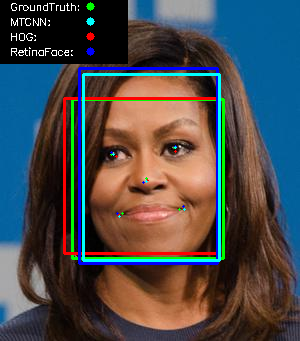
\includegraphics[width=\textwidth]{images/dlib_worst.png}
    \caption{Worst performing HOG face on average.}
    \label{dlib_worst}
  \end{minipage}
  \hfill
  \end{figure}
% As can be seen by the errors at threshold graphs, the DLIB algorithm and MTCNN algorithm show slight bias towards represented faces performing better. This is more evident in the MTCNN algorithm as throughout all thresholds there are consistently more errors with underrepresented faces.
The HOG algorithms performance after the 4 threshold indicates that it performs worst with underrepresented faces. By looking at the histograms and averages, it is clear to see that the majority of these large errors come from the mouth landmarks. This high difference could be the result of the algorithms landmark predictions being based on the bounding box generated through the HOG method. If the original bounding box prediction is inaccurate, then the likelihood of an inaccurate landmark prediction increases. The bounding box is generated through the use of HOG features which rely heavily on gradient differences to detect edges and distinguish faces. This could mean that since the gradients on a darker skin toned face differ from that of a lighter skin toned face, the algorithm could have trouble detecting the difference in gradient and the edges of the face, which would result in it being unable to place an accurate bounding box. This can be seen in Figure \ref{dlib_worst}, the bounding box is inaccurate and over estimates on the width of the face. This stems from the intensity difference between the shadows present and the skin tone on the left side of the face, resulting in difficulty for the algorithm to distinguish and detect the edge. This could be a valid reason and by looking at the bounding box overlap between the groups for the algorithm, it is clear that there is a slight difference between the accuracy of both groups. However, this difference is small, meaning that the bias is perhaps introduced somewhere else in the algorithm. The 68 point prediction is trained using the 68 point iBUG dataset (\cite{300w}). It is comprised of 135 training images annotated with 68 points. Combing through the dataset, it can be seen that 119 out of the 135 images are of represented faces. This means that the model trained to make predictions, is trained with biased data and therefore would perform worst when it comes across faces it isn't trained with. This reasoning follows that of \cite{prideorpre}, in which it is concluded that training with a specific group of data will result in better accuracy for that group, and in turn worst accuracy with any other groups that vary from the training source.
% The DLIB algorithms performance after the 4 threshold is worst for underrepresented faces and by looking at the histograms and averages its clear to see that the majority of these large errors come from the mouth landmarks. This high difference could come down to the fact that the algorithm uses pixel intensities to help guide its landmarks to the correct positions (\cite{onemilli}). The facial detection first alters the image to black and white as the algorithm doesn't require colours to work and instead uses intensity values. Since the darker skin toned faces have lower pixel intensities than lighter faces, it could mean that the algorithm would have trouble distinguishing certain features on the face and have trouble mapping the 68 points correctly. It is important to state when implementing the algorithms the DLIB algorithm was the only algorithm that used a 68 point detector as opposed to 5 point detector like the other two algorithms. This meant that the landmarks such as the eye landmarks were calculated as a representation of where they would be as opposed to the algorithm giving a prediction for them. This could result in greater inaccuracy overall for both groups which is seen when looking at the average error for the eye landmarks which is significantly higher for both groups. By looking into the worst performing DLIB face in figure \ref{dlib_worst} the differences become more apparent. Here the algorithm both overestimates the width of the face from the initial bounding box as well as underestimates the height. Since the original 68 point prediction made by the algorithm is scaled by the bounding box before being refined, it means that if there is a bad bounding box then the likelihood of an inaccurate prediction increases. The bounding box is generated through the use of HOG features which rely heavily on gradient differences to detect edges and distinguish faces. This could mean that because the gradients on a darker face differ from that of a lighter face, the algorithm could have trouble detecting the difference in gradient and the edges of the face which would result in it being unable to place an accurate bounding box. This bias exists through the design of the algorithm and is more likely i
\section{MTCNN}
The MTCNN algorithm clearly shows in the threshold graphs, that at every threshold the underrepresented faces perform worst than the represented faces. Looking into the algorithms structure, it is hard to see how a bias like this could exist within the algorithm itself. The MTCNN algorithm uses 3 networks to get bounding box and landmark coordinates. The first two networks propose and refine the bounding box with the final output network outputting the 5 landmark locations. At the start of the algorithm, the image is resized to reduce its complexity and find larger faces. This stage could be where some biased is introduced as by reducing the complexity, the algorithm could have trouble in predicting where the bounding boxes would be. However, as evident in the bounding box histogram, both groups perform very well when it comes to bounding box overlap. The algorithm doesn't use handcrafted feature descriptors like the HOG algorithm therefore, it is difficult to say that the bias exists within how the algorithm functions. Instead it is more likely the bias exists within how the algorithm was trained.

Data bias isn't a new concept within the computer vision and machine learning fields. It is when there exists a weighting or bias within the data that a model is trained with, which results in the models behaviour itself being weighted or biased (\cite{datasetbias}). In terms of the MTCNN algorithm, since the network used to predict landmark locations is trained on minimising the euclidean distance between the predicted landmarks and that ground truth landmarks. Then it is safe to assume that the training data plays a large part to why the algorithm performs in a biased way.
\begin{figure}[h!]
  \centering
  \begin{minipage}{\textwidth}
  \centering
    \includegraphics[width=0.5\textwidth]{images/celeba.png}
    \caption{Subset of avaliable attribites of CelebA dataset from: Large-scale CelebFaces Attributes (CelebA) Dataset (\cite{celeba}).}
    \label{celebattri}
  \end{minipage}
  \hfill
  \end{figure}
  
The algorithms networks are trained for face classification using the WIDER FACE dataset (\cite{widerface}), and landmark detection using the CelebA (\cite{celeba}) dataset. The landmarks are where the difference in accuracy between the groups is present. Each landmark performed worst for underrepresented faces, with the mouth landmarks showing the largest difference. Therefore, it is important to understand the composition of the CelebA dataset, as it was used for landmark training. This is a dataset consisting of 202,599 faces of 10,177 unique celebrities. Although the dataset is annotated well in terms features in the image, the annotations don't specify attributes related to race. Instead they relate to attributes like expression or face structure, a subset of these attributes are seen in figure \ref{celebattri}. This means that CelebA's annotations don't reflect human diversity well, as they fail to consider races, resulting in a biased set of annotations. A stronger reason for the algorithm performing with bias is due to the inherent sampling bias introduced by using celebrities faces in the dataset. Taking an example of Hollywood, it is generally understood that there is a lack of minority representation (\cite{hollywoo}). This is something that will therefore be reflected in a dataset such as the CelebA dataset, which contains famous celebrities. It means the algorithm is better trained to handle represented faces than it is underrepresented faces. This is because it wasn't trained using underrepresented faces, which results in failure to accurately identify features for them, and causes the algorithm to perform with a bias.
% Specifically the MTCNN algorithm was trained on the CelebA dataset which consisted of 202,599 annotated images of 10,177 unique celebrities. The images were collated from the CelebFaces dataset which contained images of celebrities that were taken from searching for celebrities names online. This resulted in the CelebA dataset containing around 20 images for each unique celebrity. This meant that the dataset then consisted of only those public figures who garnered the most internet fame to have 20 images available. This was most definitely weighted towards represented faces more than underrepresented faces as taking a simple example of Hollywood, there are more represented actors than their are underrepresented actors. Therefore its reasonable to assume that even though this dataset looks to include more ethnicity's, it still has proportionally much more represented faces which result in biased training.

\section{RetinaFace}
%heaverier wighting of featire pyramid so evertwihnt is not clean
This algorithm shows very consistent results in terms of the performance of both groups. Looking at the experiments it is clear that a bias doesn't exist within the RetinaFace algorithm, as the number of errors for represented and underrepresented faces was very similar at every threshold. The average difference at all the landmarks was also very low leaning only towards underrepresented faces performing worst at the right mouth landmark. Although, even this difference was small compared to differences shown in the other algorithms. It is important to say that the average error value for the underrepresented faces in the RetinaFace algorithm was the worst between all the algorithms, but it showed the least bias as the average error value for represented faces was very similar. This indicated that the algorithm was inaccurate for both groups. The algorithm was trained using the Wider Face (\cite{widerface}) dataset, similar to that of the MTCNN algorithm. The landmark annotations were manually annotated onto the WIDER FACE dataset, this allowed for both the face classification and landmark localisation to be trained using the same dataset. The unbiased performance could come from the fair dataset that was used to train the model. The collection method for the WIDER FACE dataset looks at different event categories like students or voters, and collates 1000 to 3000 images from the internet pertaining to these categories. This method of collection results in less of a sampling bias because the images aren't directly related to celebrities, in which there would be an inherent bias present. The spread of categories also helps include many different backgrounds and identities. However, this strong lack of bias could be a combination of both the fairer dataset and a component of the algorithm, the feature pyramid network. The FPN works by generating feature maps from the original image which contain rich semantic data, but are of a lower resolution. These maps can be used to reconstruct higher resolution layers with rich semantic information. However, due to the upsampling and downsampling of the feature maps, alot of the precise information can be lost. This means that features in images that could result in biased performance, have their complexity reduced, and the algorithm can make predictions on simpler feature maps it is better trained for. This could be a valid reason for the lack of bias, but since the algorithm is a deep learning algorithm, it is more likely that the dataset used to create the filter is responsible for the lack of bias.
% This means that when the layers are reconstructed, detail in the images are less precise, making the algorithm perform inaccurately. This inaccuracy of the algorithm with both groups results in the lack of bias because the images are reduced in complexity meaning the 

% This could be due to the complexity of certain landmarks on underrepresented faces that could introduce bias in the original image are reduced in accuracy, therefore allowing the detector to make predictions on simpler images it is better trained for.  
\section{Altering Images to Assess Dataset Bias}
\begin{figure}[h!]
  \centering
  \begin{minipage}{0.49\textwidth}
    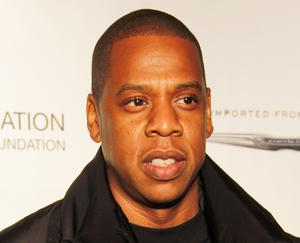
\includegraphics[width=\textwidth]{images/4_nocontrast.jpg}
    \caption{Original underrepresented face.}
    \label{4_nocontrast}
  \end{minipage}
  \hfill
  \begin{minipage}{0.49\textwidth}
    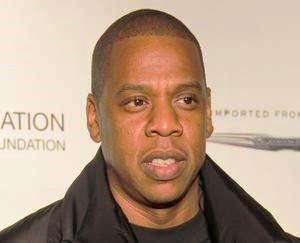
\includegraphics[width=\textwidth]{images/4_contrast.jpg}
    \caption{Lower contrast underrepresented face.}
    \label{4_contrast}
  \end{minipage}
  \hfill
\end{figure}

From the 3 algorithms it is clear to see that the MTCNN algorithm showed the most bias with its underrepresented faces performing worst compared to the represented faces. This bias seems to exist through the dataset the algorithm is trained on. For the next set of experiments, the focus was to see what factor in the underrepresented faces caused them to perform worst than the represented faces, and if the faces could be augmented such that the performance of the MTCNN algorithm could be improved. This would assist in assessing the dataset bias present.

To do this a subset of the dataset was used which had errors larger than a magnitude of 7 for the left and right mouth landmarks. These images were chosen because the mouth landmarks were the worst performing landmarks for the MTCNN algorithm. From this subset of 11 faces, 2 were represented males, 3 were underrepresented males and 6 were underrepresented females. The factor decided upon was altering the contrast of the images so that the subset of images more closely resembled the contrast of the training data. Through doing this the difference between the brightest and darkest parts of the image were reduced, this resulted in a lighter skin tone on the faces and the shadows became less pronounced. Other factors to alter such as brightness and sharpness were considered but after some testing it was found that the changing these factors impacted other parts of the image outwith the face. Every image of the subset was taken and its contrast decreased through Microsoft's image editor. This reduction in contrast led to the images being lighter in tone, with less difference between the highlights and shadows of the image. The change is visible from figure \ref{4_nocontrast} to figure \ref{4_contrast}.

\begin{table}[h!]
\centering
\begin{tabular}{|l|l|l|l|l|l|}
\hline
\textbf{id (gender/group)} & \textbf{face} & \textbf{feature} & \textbf{original} & \textbf{altered} & \textbf{difference} \\ \hline
\multirow{2}{*}{\textbf{1\_m\_m}} & \multirow{2}{*}{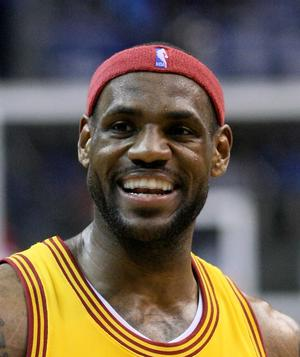
\includegraphics[width=6mm]{images/01_m_m.jpg}} & left\_mouth & 7.92 & 2.384 & 5.536 \\ \cline{3-6} 
 &  & right\_mouth & 8.615 & 3.002 & 5.613 \\ \hline
\multirow{2}{*}{\textbf{4\_m\_m}} & \multirow{2}{*}{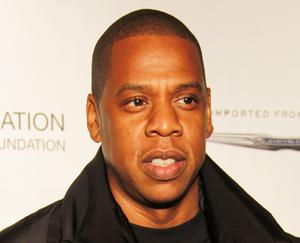
\includegraphics[width=8mm]{images/04_m_m.jpg}} & left\_mouth & 6.948 & 2.356 & 4.592 \\ \cline{3-6} 
 &  & right\_mouth & 8.075 & 3.077 & 4.998 \\ \hline
\multirow{2}{*}{\textbf{6\_m\_m}} & \multirow{2}{*}{\includegraphics[width=6mm]{images/06_m_m.jpg}} & left\_mouth & 7.48 & 3.214 & 4.266 \\ \cline{3-6} 
 &  & right\_mouth & 5.682 & 4.939 & 0.743 \\ \hline
\multirow{2}{*}{\textbf{13\_m\_r}} & \multirow{2}{*}{\includegraphics[width=6mm]{images/13_m_r.jpg}} & left\_mouth & 3.507 & 5.642 & -2.135 \\ \cline{3-6} 
 &  & right\_mouth & 9.871 & 10.8 & -0.929 \\ \hline
\multirow{2}{*}{\textbf{20\_m\_r}} & \multirow{2}{*}{\includegraphics[width=8mm]{images/20_m_r.jpg}} & left\_mouth & 7.417 & 6.915 & 0.502 \\ \cline{3-6} 
 &  & right\_mouth & 4.179 & 4.274 & -0.095 \\ \hline
\multirow{2}{*}{\textbf{27\_f\_m}} & \multirow{2}{*}{\includegraphics[width=7mm]{images/27_f_m.jpg}} & left\_mouth & 6.436 & 3.196 & 3.24 \\ \cline{3-6} 
 &  & right\_mouth & 7.292 & 6.484 & 0.808 \\ \hline
\multirow{2}{*}{\textbf{29\_f\_m}} & \multirow{2}{*}{\includegraphics[width=8mm]{images/29_f_m.jpg}} & left\_mouth & 2.001 & 1.308 & 0.693 \\ \cline{3-6} 
 &  & right\_mouth & 11.784 & 11.306 & 0.478 \\ \hline
\multirow{2}{*}{\textbf{30\_f\_m}} & \multirow{2}{*}{\includegraphics[width=6mm]{images/30_f_m.jpg}} & left\_mouth & 8.909 & 8.147 & 0.762 \\ \cline{3-6} 
 &  & right\_mouth & 0.941 & 1.186 & -0.245 \\ \hline
\multirow{2}{*}{\textbf{32\_f\_m}} & \multirow{2}{*}{\includegraphics[width=7mm]{images/32_f_m.jpg}} & left\_mouth & 2.409 & 3.808 & -1.399 \\ \cline{3-6} 
 &  & right\_mouth & 7.529 & 8.607 & 1.078 \\ \hline
\multirow{2}{*}{\textbf{33\_f\_m}} & \multirow{2}{*}{\includegraphics[width=7mm]{images/33_f_m.jpg}} & left\_mouth & 5.515 & 5.81 & -0.295 \\ \cline{3-6} 
 &  & right\_mouth & 7.898 & 7.217 & 0.681 \\ \hline
\multirow{2}{*}{\textbf{34\_f\_m}} & \multirow{2}{*}{\includegraphics[width=5.5mm]{images/34_f_m.jpg}} & left\_mouth & 7.931 & 16.856 & -8.925 \\ \cline{3-6} 
 &  & right\_mouth & 5.789 & 14.123 & -8.334 \\ \hline
\end{tabular}
\vspace*{3mm}
\caption{Error difference results from changing contrast.}
\label{results_changed}
\end{table}

% \begin{figure}[h!]
%   \centering
%   \begin{minipage}{0.7\textwidth}
%     \includegraphics[width=\textwidth]{images/results_changed.PNG}
%     \caption{Difference Results from Changing Contrast}
%     \label{results_changed}
%   \end{minipage}
%   \hfill
% \end{figure}
% Please add the following required packages to your document preamble:

\begin{figure}[h!]
  \centering
  \begin{minipage}{0.49\textwidth}
    \centering

    \includegraphics[width=0.70\textwidth]{images/lebron_result.png}
    \caption{Lebron James altered performance for MTCNN algorithm.}
    \label{lebron_result}
  \end{minipage}
  \hfill
    \begin{minipage}{0.49\textwidth}
      \centering
    \includegraphics[width=.63\textwidth]{images/bruce_result.png}
    \caption{Bruce Lee altered performance for MTCNN algorithm.}
    \label{bruce_result}
  \end{minipage}
  \hfill
\end{figure}
Running this subset of images through the MTCNN algorithm generated interesting results detailed in table \ref{results_changed}. The 3 male underrepresented faces were improved drastically by this change. Looking specifically at figure \ref{lebron_result}, we can see that the left eye error of 7.92 was reduced to 2.384 and the right mouth error of 8.615 was reduced to 3.002. The worst performing face of the algorithm was figure  \ref{bruce_result}, and by reducing the contrast of the face, the algorithm more accurately placed the landmarks. The left mouth and right mouth landmarks of 7.48 and 5.682 were reduced to 3.214 and 4.939 respectively. However, out of the 6 underrepresented women only 2 showed improvement on both landmarks, 3 showed improvement on a single landmark, and 1 performed worst on both when the images were altered. These results conclusive for the 3 underrepresented male faces were less so for female faces. This could be due to multiple factors outwith the experiment, such as facial expression and ground truth accuracy. 
\begin{figure}[h!]
  \centering
  \begin{minipage}{0.49\textwidth}
    \centering
    \includegraphics[width=0.6\textwidth]{images/whoopi_result.png}
    \caption{Whoopi Goldberg altered performance for MTCNN algorithm.}
    \label{whoopi_results}
  \end{minipage}
  \hfill
  \begin{minipage}{0.49\textwidth}
    \centering
    \includegraphics[width=0.61\textwidth]{images/lupita_result.png}
    \caption{Lupita Nyong'o altered performance for MTCNN algorithm.}
    \label{lupita_result}
  \end{minipage}
  \hfill
\end{figure}

For example figure \ref{whoopi_results}, showed a large smile which could effect the accuracy. This is because the algorithm could have a lack of training with expressions at this contrast, where the difference between the teeth and the lips is less pronounced. The ground truth accuracy also affected the results of the experiment. With certain faces like figure \ref{lupita_result}, the ground truth was slightly inaccurate. This means that the accuracy calculated could've shown improvement for both landmarks, but since the ground truth wasn't accurate, this improvement wasn't reflected properly. Even with these results for females, it is still evident that changing the contrast did overall have a positive influence in the algorithms performance. This further emphasises that a bias does exist within the data the algorithm was trained on, as by augmenting a subset of the images to resemble closer to the represented faces. The algorithm was able to provide a better performance for the majority of them.
\section{Components of Bias}
The results do indicate a bias existing within the MTCNN, and to a lesser degree that HOG and Viola-Jones algorithm. However, the algorithms have different reasons for why the bias could exist and by looking at these it is clear to distinguish two main components that can introduce bias. This is the bias introduced by the design of the algorithm, and the bias introduced through the dataset the algorithm is trained on. The design of the older algorithms like HOG and Viola-Jones are part of the former category because of their manually constructed filter and feature descriptors. The feature descriptors used for these algorithms could be encoded to use information from the image which varies between represented and underrepresented faces, like pixel intensity. This would mean the feature extracted for a represented face, might not be extracted for a underrepresented one causing the filter to behave differently between the groups. The MTCNN algorithm introduces bias through the latter category as the filter isn't directly created with pre-existing domain knowledge which could introduce bias, but instead the filter is created automatically using the learning task and training data. This means that there is more emphasis on the training data being the root cause for bias being introduced in the CNN methods. This is seen by improvement to the results after altering the contrast of the images to resemble the training data faces.

\section{Dataset Bias}
Dataset bias is the prevalent bias present in CNN methods. There are two reasons it exists. Its introduction through sampling bias, and its lack of mitigation through benchmark datasets.

% Dataset bias is an important factor to consider, if all modern CNN methods can fall victim to it. Understanding how the images are collated should lead to understanding how the bias is introduced. In the same sense that understanding how the algorithms are evaluated should assist in understanding why the bias still exists and hasn't been mitigated.
% It should be noted that it is not introduced purposefully to discriminate against a certain group. Its often introduced indirectly into algorithms through how the faces have been collated. However, when it is introduced, it can be very difficult to evaluate that it exists and remove it. 
%intricaies are lost
%==================================================================================================================================
% \chapter{Dataset Bias}
% \section{Introducing Bias}
% The largest contributing factor to bias within modern deep learning facial detection algorithms is the data they are trained with. The older algorithms like the Viola Jones algorithm (\cite{viola}) and HOG detectors (\cite{hog}) relied heavily on extracting features within the image and using handcrafted classifiers to help understand what was within the image. The Viola Jones algorithm specifically looked at regions of intensity in an image and created Haar-like features so that it could detect landmarks in the image and the HOG detector used histograms of the oriented gradients within an image. These algorithms which rely heavily on features are more prone to bias through the algorithm design, as the semantic information being taken from the images can directly be altered by features present in underrepresented faces that are not in represented faces like darker skin tone for example. The modern day algorithms rely on convolution neural networks for face detection and recognition tasks which step away from specific feature extraction and instead look to train a CNN for facial detection tasks (\cite{mtcnn},\cite{retinaface}). The CNN algorithms heavily rely on training data and this reflects on their performance. If an algorithm is trained on data that predominantly contains represented faces then when the algorithm is presented with an underrepresented face, it will be a case it is not prepared for and in turn will be unable to provide accurate results. 
% \subsection{Lack of Available Datasets}
% There is an extreme lack of datasets available which look to remove bias through having a collection of faces more representative than just a small subset of the population. At the onset of facial detection there wasn't much consideration into reducing bias because the goal early on was to improve detection accuracy and performance against benchmark datasets. The early training datasets created consisted of photos with challenging characteristics such as pose, expression or illumination. Race wasnt a characteristic that was annotated or placed in early datasetsCorrecting bias wasn't a consideration until the algorithms saw more use in real world scenarios where it became apparent that this was a large issue (\cite{nist}). The lack of datasets is 
\subsection{Sampling Bias}
Dataset sampling bias occurs when collating images for a dataset. It is the result of collecting images in a way such that the images don't have an equal probability to be selected. The most common form of sampling bias present in datasets is related to sampling celebrities. This is exhibited in many datasets such as the CelebA (\cite{celeba}), VGGFace2 (\cite{vggface2}) and PubFig (\cite{pubfig}) datasets. Specifically looking at the popular evaluation dataset, VGGFace2. It consists of 3.31 million images. The images were collated from Google image search and contain varying pose, age and most importantly ethnicity. From the 3.31 million images, there are only 9131 distinct faces. These distinct faces were chosen from an initial list of 500,000 public figures from the the Freebase knowledge graph (\cite{freebase}). The list was reduced in size by removing those names which didn't have enough credible photos along with them. This meant that the list then consisted of only those public figures who garnered the most fame. This was weighted towards represented faces more than underrepresented faces as looking at popular figures in terms of actors in Hollywood movies, there are more represented actors than their are underrepresented actors by a massive margin (\cite{hollywoo}). Therefore, it is reasonable to assume that even though this dataset looks to include more ethnicities, it still has proportionally more represented faces which results in biased training. However, the sampling bias present in datasets doesn't only come from celebrities, as the bias can be introduced indirectly when the dataset only looks at a specific category of person. The PPB dataset from \cite{gendershades}, looks to reduce bias for race and gender by using images of parliamentary members around the world. They succeed in reducing this bias present in the dataset but indirectly introduce another bias. Since all the faces are of parliamentary members, there is a large age bias present because the dataset doesn't contain any young faces. This shows the difficulties in using any specific category to  create a dataset, as sampling bias can easily and indirectly be introduced. 

% There is an inherent sampling bias present in many datasets. These datasets created consist of images collated from the internet of celebrities and other popular faces. This introduces an inherent bias because by sampling from  celebrities, then there will be a larger proportion of represented faces as proportionally there are less celebrities belonging to minorities. This is why its exhibited in many datasets such as the CelebA (\cite{celeba}), VGGFace2 (\cite{vggface2}) and PubFig (\cite{pubfig}) datasets. Specifically looking at the popular evaluation dataset, VGGFace2. It consists of 3.31 million images. The images were collated from Google image search and contain varying pose, age and most importantly ethnicity. From the 3.31 million images, there are only 9131 distinct faces. These distinct faces were chosen from an initial list of 500,000 public figures from the the Freebase knowledge graph. The list was reduced in size by removing those names which didn't have enough credible photos along with them. This meant that the list then consisted of only those public figures who garnered the most fame. This was weighted towards represented faces more than underrepresented faces as looking at popular figures in terms of actors in Hollywood movies, there are more represented actors than their are underrepresented actors by a massive margin (\cite{hollywoo}). Therefore its reasonable to assume that even though this dataset looks to include more ethnicities, it still has proportionally much more represented faces which results in biased training. The sampling bias present in datasets doesn't only come from celebrities, as the bias can be introduced indirectly when the dataset only looks at a specific category of person. The PPB dataset from \cite{gendershades}, looks to reduce bias for race and gender by using images of parliamentary members around the world. They succeed in reducing this bias present in the dataset but indirectly introduce another bias. Since all the faces are of parliamentary members, there is a large age bias present, as the dataset doesn't contain any young faces. This shows the difficulties in using any specific category to  create a dataset, as sampling bias can easily and indirectly be introduced. This is one of the main reasons bias is introduced into algorithms because there are not enough unbiased datasets available due to sampling bias.
The Diversity in Faces paper (\cite{dif}), analysed a number of widely available and popular face datasets. It went through each dataset and looked at the number of males, females and type of skin tones present in them. The findings were conclusive and showed that for every dataset considered, there was a higher percentage of lighter skin tone faces than darker skin tones (Table \ref{diftable}). The Pubfig dataset described above does result in a very uneven skew of skin tone as only 18\% of the dataset contains underrepresented faces with a darker skin tone. This is due to the sampling bias. The same is seen with the CelebA dataset, which the MTCNN algorithm uses to train its landmark localisation with. It is one of the least diversified datasets with only 14.2\% of images being of darker toned underrepresented individuals. It is important to take these results with a level of uncertainty because the Diversity in Faces paper has not yet been published, and the methodology behind how the results were gathered isn't entirely explained. However, these results do indicate a massive skew in the skin tone diversity of these datasets, which provides reasonable evidence to a sampling bias being present.
\begin{table}[h!]
\centering
\begin{minipage}{\textwidth}
\centering
\begin{tabular}{|l|l|l|l|l|}
\hline
\textbf{} & \multicolumn{2}{l|}{\textbf{Gender}} & \multicolumn{2}{l|}{\textbf{Skin Color/Type}} \\ \hline
\textbf{Dataset} & \textbf{Female} & \textbf{Male} & \textbf{Darker} & \textbf{Lighter} \\ \hline
LFW (\cite{300w}) & 22.5\% & 77.4\% & 18.8\% & 81.2\% \\ \hline
IJB-C (\cite{ijb-c}) & 37.4\% & 62.7\% & 18.0\% & 82.0\% \\ \hline
Pubfig (\cite{pubfig}) & 50.8\% & 49.2\% & 18.0\% & 82.0\% \\ \hline
CelebA (\cite{celeba})& 58.1\% & 42.0\% & 14.2\% & 85.8\% \\ \hline
UTKface (\cite{utkface}) & 47.8\% & 52.2\% & 35.6\% & 64.4\% \\ \hline
AgeDB (\cite{agedb}) & 40.6\% & 59.5\% & 5.4\% & 94.6\% \\ \hline
PPB (\cite{gendershades})& 44.6\% & 55.4\% & 46.4\% & 53.6\% \\ \hline
IMDB-Face (\cite{imdb}) & 45.0\% & 55.0\% & 12.0\% & 88.0\% \\ \hline
\end{tabular}
\vspace*{3mm}
\centering
\caption{Distribution of gender and skin color/type for seven prominent face image datasets From: Diversity in Faces (\cite{dif}). }
\label{diftable}
\end{minipage}
\end{table}

% Specifically the MTCNN algorithm was trained on the CelebA dataset which consisted of 202,599 annotated images of 10,177 unique celebrities. The images were collated from the CelebFaces dataset which contained images of celebrities that were taken from searching for celebrities names online. This resulted in the CelebA dataset containing around 20 images for each unique celebrity. This meant that the dataset then consisted of only those public figures who garnered the most internet fame to have 20 images available. This was most definitely weighted towards represented faces more than underrepresented faces as taking a simple example of Hollywood, there are more represented actors than their are underrepresented actors. Therefore its reasonable to assume that even though this dataset looks to include more ethnicity's, it still has proportionally much more represented faces which result in biased training.

% Specifically the MTCNN algorithm was trained on the VGGFace2 dataset which consisted of 3.31 million images. The images were collated from Google image search and consisted of varying pose, age and most importantly ethnicity. From the 3.31 million images there are only 9131 distinct faces. These distinct faces were chosen from an initial list of 500k public figures from the the Freebase knowledge graph. The list was reduced in size by removing those names which didn't have enough credible photos along with it. This meant that the list then consisted of only those public figures who garnered the most internet fame. This was most definitely weighted towards represented faces more than underrepresented faces as taking a simple example of Hollywood, there are more represented actors than their are underrepresented actors. Therefore its reasonable to assume that even though this dataset looks to include more ethnicity's, it still has proportionally much more represented faces which result in biased training.
\subsection{Benchmark Datasets}
The Labelled Faces in the Wild dataset (\cite{300w}) is a popular dataset amongst algorithms and frameworks as it is a benchmark dataset used to evaluate accuracy and robustness. A reason for its popularity is that it contains images of faces in unconstrained environments, with differing pose, expression and shadows. An assumption would be that a popular dataset used to evaluate the robustness of face detection performance "in the wild" would be representative of the real world, but in reality this dataset has many issues. These being that the dataset lacks representation of minorities as well as women, kids and the elderly. Benchmark datasets like this are a large reason to why bias exists within face detection algorithms. They aren't being used to train the algorithms directly but they are being used to evaluate them. This means that potentially biased algorithms are being evaluated against a dataset that doesn't consider bias. This results in high accuracy scores for these algorithms and indicates to others that they are accurate. This is occlusive to the real underlying issues and indirectly increases the bias present. Since there is no evaluation of the bias, it is not being mitigated and algorithms continue to use the same biased datasets resulting in biased performance. 
\section{Research Question}
% Underrepresented faces with a darker skin tone could cause the algorithm to misidentify the edges of a face which results in a biased result as faces of varying brightness would be treated differently.
To answer if there exists a bias within the face detection field is simple as both the results and research indicates that a bias exists in the scene towards both race and gender. This is evident from the difference in accuracy between the represented and underrepresented faces. To answer why there exists a bias is a more complicated question. There doesn't exist a bias within all the algorithms, therefore it isn't as straightforward as finding one factor across every algorithm that could introduce the bias. Instead each algorithm has to be specifically analysed to understand how the bias exists. Through doing so it is seen that bias can be introduced into the algorithms in two ways. One is through the design of the algorithm and the other is through the dataset which the algorithm is trained on. 

The Viola-Jones and HOG algorithms showed bias through both their design and dataset. The algorithms feature descriptors look directly at differences in brightness which could vary between groups, resulting in an algorithmic bias present in the design of the feature descriptors. The dataset bias was introduced through using datasets that lacked underrepresented faces. In the case of Viola-Jones this was assumed due to its foundational nature, and in the case of HOG. The 68 point iBUG dataset (\cite{300w}), only consisted of only 12\% underrepresented faces. The RetinaFace and MTCNN algorithms both showed sensitivity to bias through mainly the dataset they were trained on, instead of their design. The RetinaFace algorithm showed no bias due to being trained with the WIDER FACE dataset (\cite{widerface}), that contained a wide distribution of different genders and races. This was achieved through the sampling methodology, which looked at different events to ensure a wider range of genders and ethnic backgrounds. It was thought that the feature pyramid network present could reduce bias, but since the algorithm is a deep learning algorithm. It was likely that the dataset used to create the filter was responsible for the lack of bias. The MTCNN algorithm showed major bias due to being trained on the inherently biased CelebA dataset (\cite{celeba}). This bias was the result of sampling bias present when collating the images. Altering the worst performing images for the algorithm to match the characteristics of the training dataset, resulted in improved performance which emphasised the presence of dataset bias. The dataset bias present in the majority of the algorithms comes from two main factors. Its introduction through sampling bias and its lack of mitigation through benchmark dataset bias. These two factors create a cycle where algorithms using biased datasets are being evaluated as accurate by biased benchmark datasets. This results in the algorithms and datasets being perceived as accurate and implemented, even though there exists a bias.

It is clear that the image-based methods of MTCNN and RetinaFace introduce bias, or lack of bias through their dataset. Whereas the feature-based methods show more sensitivity to bias through their design. However, this isn't exclusive as analysis of the Viola-Jones and HOG algorithm indicate that dataset bias is still present.
% results gathered it can be seen that bias is introduced through two main means, dataset bias and
% algorithmic bias. Image based methods seem to be more sensitive to dataset bias, compared to
% feature based methods having more sensitivity to algorithmic bias. This however isn’t exclusive
% as the results of the paper show that components of deep learning methods still have an effect on
% their performance in relation to bias

% Through analysis of the HOG and Viola-Jones algorithms its evident that the bias is introduced through the design as well as the dataset. The algorithms feature descriptors look directly at differences in brightness which could vary between groups, resulting in an algorithmic bias. The dataset bias is introduced with the lack of underrepresented faces in the training data. The deep learning approaches of RetinaFace and MTCNN both show sensitivity to bias through their datasets

% This differs from the deep learning approaches of MTCNN and RetinaFace which show sensitivity to bias through the dataset the algorithm is trained with, more than the design of the algorithm. However, the results show that this isn't the only factor which affects the bias present in the algorithms as although both methods are deep learning CNN's, they have opposing performance when it comes to bias. The RetinaFace algorithm shows little to no bias existing as both groups perform equally. This isn't due to only the training data, as looking into the algorithm it uses a feature pyramid network. This component could reduce the bias as its upsampling and downsampling of the image could reduce the complexity of certain features that the dataset bias would introduce. The MTCNN algorithm doesn't use a FPN and exhibits the largest bias between all the algorithms. This bias exists due to the training data the algorithm was trained on being bias towards more represented faces than underrepresented faces. Altering the underrepresented faces such that they have simmilar contrast to the represented faces resulted in an improvement of some capacity to the accuracy. This further emphasised the effect of dataset bias to the CNN method. The reasons behind dataset bias come down to two factors, its introduction and its lack of mitigation. Its introduction comes from the inherent sampling bias present when creating the large datasets, which result in their being more represented faces than underrepresented faces. The lack of mitigation comes from the lack of benchmark datasets which evaluate the race and gender bias. This creates a cycle where datasets are being created through biased sampling, they are then being evaluated as accurate against a biased benchmark dataset, which results in more datasets being created following the same methodology. These factors combined are the largest reason to why dataset bias exists.

 

\section{Limitations of Results}
%size of dataset was small so reasoning is weak
%Lack of expeiremnts with landmarks for mtcnn
%
%Ground trruth accuracy
The results and evaluation of the algorithms had limitations associated with them. The limited size of the dataset meant that the results gathered had a higher variance within them. This variance affected the strength of the analysis and reasoning on why a bias existed as it was based on a small sample size. The analysis behind the feature-based algorithms poor performance is also not as strong as it could be. Further testing could've been done to see if altering the intensity of pixels would affect the feature extraction for the HOG and Viola-Jones algorithm. This would provide stronger evidence to the bias being present in the design of the algorithms. 
% Being accurate against a biased dataset only infers that the algorithm is accurate against a bias. To truly look at an algorithms accuracy in the wild, it should be evaluated against a dataset that is actually representative of the wild. This means the dataset should be diverse with races, gender and ages and not only expression, pose or illumination, which is the trap many benchmark datasets like LFW fall into.

% This serves as a reminder that even if your algorithm is accurate against a benchmark dataset like 300 AFLW this doesnt equate to it being accurate or unbiased. This is because being accurate against a bias dataset only means your algorithm is only accurate against a bias and to truly look at an algorithms accuracy it should be evaluated against a fairly weighted data set. The focus should be on including gender and race into accuracy as for an algorithm to have good "in the wild" performance then it should be able to perform with different races and genders as this is what it will encounter outwith its testing environment.

%talk about the dataset widerfaec and styff
% \section{Training}
% The 3 algorithms are all trained on different data sets. the DLIB algorithm is trained on the iBUG 300-W dataset which consisted of 135 images varying in pose and illumination. These images considered to be difficult are used to train the algorithm so that its accuracy is less affected by various factors. This dataset doesnt look to reduce bias at all, there is not an even number of males and females or represented and underrepresented faces. 
% The MTCNN algorithm was trained on the VGGFace2 dataset which consisted of 3.31 million images. The images were collated from Google image search and consisted of varying pose, age and most importantly ethnicity. How can a dataset that actively pursues varying ethnicity's then perform with a bias. I think this is due to how the faces were selected. From the 3.31 million images there are only 9131 distinct faces. These distinct faces were chosen from an initial list of 500k public figures from the the Freebase knowledge graph. The list was reduced in size by removing those names which didn't have enough credible photos along with it. This meant that the list then consisted of only those public figures who garnered the most internet fame. This was most definitely weighted towards represented faces more than underrepresented faces as taking a simple example of Hollywood, there are more represented actors than their are underrepresented actors. Therefore its reasonable to assume that even though this dataset looks to include more ethnicity's, it still has proportionally much more represented faces which result in biased training.
% \section{IBM: Diversity in Faces}
% \subsection{Coding Schemes}
% However there are some datasets that look to reduce the bias completely and provide enough images to train models to work better in the real world. IBM's Diveristy in Faces dataset is one such example (\cite{dif}). Here diversity in faces isn't reduced to only ethnicity or gender which some other datasets conclude is representative but instead diversity is put down to 10 different coding schemes which include gender, age, skin colour, facial symmetry and different craniofacial differences to name a few. This dataset looks to have an even distribution of faces according to their different coding schemes. This approach to diversity would mean a largely unbiased dataset as diversity is being statistically measured to ensure that the different factors that result in diversity are being evenly distributed. Algorithms training on this type of dataset would perform with much less bias as its not inherently being introduced at the training stage so any bias that exists would be within the algorithm itself. 
% \subsection{Dataset Groups}
% \begin{table}[h!]
% \centering
% \begin{minipage}{\textwidth}
% \centering
% \begin{tabular}{|l|l|l|l|l|}
% \hline
% \textbf{} & \multicolumn{2}{l|}{\textbf{Gender}} & \multicolumn{2}{l|}{\textbf{Skin Color/Type}} \\ \hline
% \textbf{Dataset} & \textbf{Female} & \textbf{Male} & \textbf{Darker} & \textbf{Lighter} \\ \hline
% LFW (\cite{300w}) & 22.5\% & 77.4\% & 18.8\% & 81.2\% \\ \hline
% IJB-C (\cite{ijb-c}) & 37.4\% & 62.7\% & 18.0\% & 82.0\% \\ \hline
% Pubfig (\cite{pubfig}) & 50.8\% & 49.2\% & 18.0\% & 82.0\% \\ \hline
% CelebA (\cite{celeba})& 58.1\% & 42.0\% & 14.2\% & 85.8\% \\ \hline
% UTKface (\cite{utkface}) & 47.8\% & 52.2\% & 35.6\% & 64.4\% \\ \hline
% AgeDB (\cite{agedb}) & 40.6\% & 59.5\% & 5.4\% & 94.6\% \\ \hline
% PPB (\cite{gendershades})& 44.6\% & 55.4\% & 46.4\% & 53.6\% \\ \hline
% IMDB-Face (\cite{imdb}) & 45.0\% & 55.0\% & 12.0\% & 88.0\% \\ \hline
% \end{tabular}
% \vspace*{3mm}
% \centering
% \caption{Distribution of Gender and Skin Color/Type for Seven Prominent Face Image Datasets From: Diversity in Faces (\cite{dif}) }
% \end{minipage}
% \end{table}
% The paper proposed alongside the dataset, analysed a number of widely available and popular face datasets. It went through each dataset and looked at the number of males, females and type of skin tones present in them. The findings were conclusive and showed that for every dataset considered there was a higher percentage of lighter skin tone faces than darker skin tones. The CelebA dataset which the MTCNN algorithm uses to train its landmark localisation with, was one of the least diversified datasets with only 14.2\% of images being of darker toned underrepresented individuals. The popular LFW dataset lacks diversity not only in small percentage of darker skin tones at 18.8\%, but also in its lack of females with only 22.5\% of the dataset containing females. It is important to take these results as not absolute because the paper itself hasn't been peer reviewed and the methodology behind how the results were gathered isn't entirely explained. However these results do indicate a massive skew in the skin tone diversity of these datasets, and to a lesser extent the skew in gender.



%==================================================================================================================================
\chapter{Conclusion}

\section{Summary}
This paper provided research into facial detection algorithms to investigate if and why there existed a bias towards race and gender. A novel dataset called the 5025 dataset was compiled consisting of an equal number of genders and representations for faces. Each algorithms performance was measured against represented and underrepresented faces within the dataset. The difference between the performance of the algorithms with these groups indicated if a bias was present. The results showed that a slight bias existed within the Viola-Jones and HOG algorithms due to their feature descriptors and training data. The MTCNN algorithm showed the largest bias due to its dataset, and the RetinaFace algorithm had the smallest difference between the groups, indicating that a bias wasn't present. This was because of its training data. The dataset factor of face detection was researched and it was found that the bias existed due to its introduction from sampling bias, and its lack of mitigation through biased benchmark datasets. 

% The dataset factor of face detection was researched and it was found that the sampling bias present in datasets used by algorithms affected their performance against underrepresented faces. The lack of underrepresented faces in benchmark datasets also meant that algorithms were being deemed accurate for real world use, even though their bias wasn't being evaluated.

\section{Future Work}
Due to the scope of the project along with the complexity of the face detection algorithms, there were many factors that were unable to be isolated and tested. Therefore, this leaves much room for further work, which includes:
\begin{itemize}
  \item Expand on face detection field by evaluating other algorithms with differing features like the R-CNN family of algorithms (\cite{rcnn}) or YOLO framework (\cite{yolo}). 
  \item Evaluate the algorithms on a larger dataset comprising of an evenly distributed number of represented and underrepresented faces.
  \item Isolate the results by gender to get insight into specifically the gender bias instead of the race and gender bias combined.
  \item Retrain the MTCNN algorithm using a fairer dataset to evaluate if there is any improvement against reducing the bias present.
\end{itemize}
These are the main directions that future work could be taken in. All try to improve the understanding behind the existence of bias, and work on bringing more robustness to the results. However, the most important consideration for any proposed future work is to continue a dialogue within the face detection field about the existence of bias, as it is only with understanding why the bias exists that it can be mitigated and fairness can be ensured.
% Directions for future work include further research into trying other possible algorithms that exhibit differing structures from the 4 described in this project. Potential algorithms include the R-CNN family of algorithms and the YOLO Framework, both of which were viable for this project but were unable to be implemented due to time constraints. The dataset bias for the MTCNN algorithm was explored but it could be extended by retraining the algorithm with a fairer dataset to see if it had any impact in reducing the bias present. It would also be interesting to extend the evaluation of the algorithms by using other datasets of a larger size 





% and was due in part to the feature pyramid network which through upsampling and downsampling could reduce the complexity in faces such that they were treated with less of a bias. The MCTNN algorithm showed the greatest difference between the groups and through inspection of the algorithm it was clear the dataset had a part to play. The underrepresented faces were then altered such that the reduction of contrast would make them similar to the represented faces and after doing so an improvement was seen in the performance of the MTCNN algorithm, further emphasising the effect the training data had. The paper also looked into the dataset bias that existed for algorithms

%==================================================================================================================================


% \chapter{Analysis/Requirements}
% What is the problem that you want to solve, and how did you arrive at it?
% \section{Guidance}
% Make it clear how you derived the constrained form of your problem via a clear and logical process. 

% %==================================================================================================================================
% \chapter{Design}
% How is this problem to be approached, without reference to specific implementation details? 
% \section{Guidance}
% Design should cover the abstract design in such a way that someone else might be able to do what you did, but with a different language or library or tool.

% %==================================================================================================================================
% \chapter{Implementation}
% What did you do to implement this idea, and what technical achievements did you make?
% \section{Guidance}
% You can't talk about everything. Cover the high level first, then cover important, relevant or impressive details.



% \section{General points}
% \begin{figure}[h!]
%   \centering
%   \begin{minipage}{0.49\textwidth}
%     \includegraphics[width=\textwidth]{images/dlib_box.png}
%     \caption{Bounding Box IoU Histogram DLIB}
%     \label{dlib_box}
%   \end{minipage}
%  \end{figure}
% These points apply to the whole dissertation, not just this chapter.



% \subsection{Figures}
% \emph{Always} refer to figures included, like Figure \ref{fig:relu}, in the body of the text. Include full, explanatory captions and make sure the figures look good on the page.
% You may include multiple figures in one float, as in Figure \ref{fig:synthetic}, using \texttt{subcaption}, which is enabled in the template.



% % Figures are important. Use them well.
% \begin{figure}
%     \centering
%     \includegraphics[width=0.5\linewidth]{images/relu.pdf}    

%     \caption{In figure captions, explain what the reader is looking at: ``A schematic of the rectifying linear unit, where $a$ is the output amplitude,
%     $d$ is a configurable dead-zone, and $Z_j$ is the input signal'', as well as why the reader is looking at this: 
%     ``It is notable that there is no activation \emph{at all} below 0, which explains our initial results.'' 
%     \textbf{Use vector image formats (.pdf) where possible}. Size figures appropriately, and do not make them over-large or too small to read.
%     }

%     % use the notation fig:name to cross reference a figure
%     \label{fig:relu} 
% \end{figure}


% \begin{figure}
%     \centering
%     \begin{subfigure}[b]{0.45\textwidth}
%         \includegraphics[width=\textwidth]{images/synthetic.png}
%         \caption{Synthetic image, black on white.}
%         \label{fig:syn1}
%     \end{subfigure}
%     ~ %add desired spacing between images, e. g. ~, \quad, \qquad, \hfill etc. 
%       %(or a blank line to force the subfigure onto a new line)
%     \begin{subfigure}[b]{0.45\textwidth}
%         \includegraphics[width=\textwidth]{images/synthetic_2.png}
%         \caption{Synthetic image, white on black.}
%         \label{fig:syn2}
%     \end{subfigure}
%     ~ %add desired spacing between images, e. g. ~, \quad, \qquad, \hfill etc. 
%     %(or a blank line to force the subfigure onto a new line)    
%     \caption{Synthetic test images for edge detection algorithms. \subref{fig:syn1} shows various gray levels that require an adaptive algorithm. \subref{fig:syn2}
%     shows more challenging edge detection tests that have crossing lines. Fusing these into full segments typically requires algorithms like the Hough transform.
%     This is an example of using subfigures, with \texttt{subref}s in the caption.
%     }\label{fig:synthetic}
% \end{figure}

% \clearpage

% \subsection{Equations}

% Equations should be typeset correctly and precisely. Make sure you get parenthesis sizing correct, and punctuate equations correctly 
% (the comma is important and goes \textit{inside} the equation block). Explain any symbols used clearly if not defined earlier. 

% For example, we might define:
% \begin{equation}
%     \hat{f}(\xi) = \frac{1}{2}\left[ \int_{-\infty}^{\infty} f(x) e^{2\pi i x \xi} \right],
% \end{equation}    
% where $\hat{f}(\xi)$ is the Fourier transform of the time domain signal $f(x)$.

% \subsection{Algorithms}
% Algorithms can be set using \texttt{algorithm2e}, as in Algorithm \ref{alg:metropolis}.

% % NOTE: line ends are denoted by \; in algorithm2e
% \begin{algorithm}
%     \DontPrintSemicolon
%     \KwData{$f_X(x)$, a probability density function returing the density at $x$.\; $\sigma$ a standard deviation specifying the spread of the proposal distribution.\;
%     $x_0$, an initial starting condition.}
%     \KwResult{$s=[x_1, x_2, \dots, x_n]$, $n$ samples approximately drawn from a distribution with PDF $f_X(x)$.}
%     \Begin{
%         $s \longleftarrow []$\;
%         $p \longleftarrow f_X(x)$\;
%         $i \longleftarrow 0$\;
%         \While{$i < n$}
%         {
%             $x^\prime \longleftarrow \mathcal{N}(x, \sigma^2)$\;
%             $p^\prime \longleftarrow f_X(x^\prime)$\;
%             $a \longleftarrow \frac{p^\prime}{p}$\;
%             $r \longleftarrow U(0,1)$\;
%             \If{$r<a$}
%             {
%                 $x \longleftarrow x^\prime$\;
%                 $p \longleftarrow f_X(x)$\;
%                 $i \longleftarrow i+1$\;
%                 append $x$ to $s$\;
%             }
%         }
%     }
    
% \caption{The Metropolis-Hastings MCMC algorithm for drawing samples from arbitrary probability distributions, 
% specialised for normal proposal distributions $q(x^\prime|x) = \mathcal{N}(x, \sigma^2)$. The symmetry of the normal distribution means the acceptance rule takes the simplified form.}\label{alg:metropolis}
% \end{algorithm}

% \subsection{Tables}

% If you need to include tables, like Table \ref{tab:operators}, use a tool like https://www.tablesgenerator.com/ to generate the table as it is
% extremely tedious otherwise. 

% \begin{table}[]
%     \caption{The standard table of operators in Python, along with their functional equivalents from the \texttt{operator} package. Note that table
%     captions go above the table, not below. Do not add additional rules/lines to tables. }\label{tab:operators}
%     %\tt 
%     \rowcolors{2}{}{gray!3}
%     \begin{tabular}{@{}lll@{}}
%     %\toprule
%     \textbf{Operation}    & \textbf{Syntax}                & \textbf{Function}                            \\ %\midrule % optional rule for header
%     Addition              & \texttt{a + b}                          & \texttt{add(a, b)}                                    \\
%     Concatenation         & \texttt{seq1 + seq2}                    & \texttt{concat(seq1, seq2)}                           \\
%     Containment Test      & \texttt{obj in seq}                     & \texttt{contains(seq, obj)}                           \\
%     Division              & \texttt{a / b}                          & \texttt{div(a, b) }  \\
%     Division              & \texttt{a / b}                          & \texttt{truediv(a, b) } \\
%     Division              & \texttt{a // b}                         & \texttt{floordiv(a, b)}                               \\
%     Bitwise And           & \texttt{a \& b}                         & \texttt{and\_(a, b)}                                  \\
%     Bitwise Exclusive Or  & \texttt{a \textasciicircum b}           & \texttt{xor(a, b)}                                    \\
%     Bitwise Inversion     & \texttt{$\sim$a}                        & \texttt{invert(a)}                                    \\
%     Bitwise Or            & \texttt{a | b}                          & \texttt{or\_(a, b)}                                   \\
%     Exponentiation        & \texttt{a ** b}                         & \texttt{pow(a, b)}                                    \\
%     Identity              & \texttt{a is b}                         & \texttt{is\_(a, b)}                                   \\
%     Identity              & \texttt{a is not b}                     & \texttt{is\_not(a, b)}                                \\
%     Indexed Assignment    & \texttt{obj{[}k{]} = v}                 & \texttt{setitem(obj, k, v)}                           \\
%     Indexed Deletion      & \texttt{del obj{[}k{]}}                 & \texttt{delitem(obj, k)}                              \\
%     Indexing              & \texttt{obj{[}k{]}}                     & \texttt{getitem(obj, k)}                              \\
%     Left Shift            & \texttt{a \textless{}\textless b}       & \texttt{lshift(a, b)}                                 \\
%     Modulo                & \texttt{a \% b}                         & \texttt{mod(a, b)}                                    \\
%     Multiplication        & \texttt{a * b}                          & \texttt{mul(a, b)}                                    \\
%     Negation (Arithmetic) & \texttt{- a}                            & \texttt{neg(a)}                                       \\
%     Negation (Logical)    & \texttt{not a}                          & \texttt{not\_(a)}                                     \\
%     Positive              & \texttt{+ a}                            & \texttt{pos(a)}                                       \\
%     Right Shift           & \texttt{a \textgreater{}\textgreater b} & \texttt{rshift(a, b)}                                 \\
%     Sequence Repetition   & \texttt{seq * i}                        & \texttt{repeat(seq, i)}                               \\
%     Slice Assignment      & \texttt{seq{[}i:j{]} = values}          & \texttt{setitem(seq, slice(i, j), values)}            \\
%     Slice Deletion        & \texttt{del seq{[}i:j{]}}               & \texttt{delitem(seq, slice(i, j))}                    \\
%     Slicing               & \texttt{seq{[}i:j{]}}                   & \texttt{getitem(seq, slice(i, j))}                    \\
%     String Formatting     & \texttt{s \% obj}                       & \texttt{mod(s, obj)}                                  \\
%     Subtraction           & \texttt{a - b}                          & \texttt{sub(a, b)}                                    \\
%     Truth Test            & \texttt{obj}                            & \texttt{truth(obj)}                                   \\
%     Ordering              & \texttt{a \textless b}                  & \texttt{lt(a, b)}                                     \\
%     Ordering              & \texttt{a \textless{}= b}               & \texttt{le(a, b)}                                     \\
%     % \bottomrule
%     \end{tabular}
%     \end{table}
% \subsection{Code}

% Avoid putting large blocks of code in the report (more than a page in one block, for example). Use syntax highlighting if possible, as in Listing \ref{lst:callahan}.

% \begin{lstlisting}[language=python, float, caption={The algorithm for packing the $3\times 3$ outer-totalistic binary CA successor rule into a 
%     $16\times 16\times 16\times 16$ 4 bit lookup table, running an equivalent, notionally 16-state $2\times 2$ CA.}, label=lst:callahan]
%     def create_callahan_table(rule="b3s23"):
%         """Generate the lookup table for the cells."""        
%         s_table = np.zeros((16, 16, 16, 16), dtype=np.uint8)
%         birth, survive = parse_rule(rule)

%         # generate all 16 bit strings
%         for iv in range(65536):
%             bv = [(iv >> z) & 1 for z in range(16)]
%             a, b, c, d, e, f, g, h, i, j, k, l, m, n, o, p = bv

%             # compute next state of the inner 2x2
%             nw = apply_rule(f, a, b, c, e, g, i, j, k)
%             ne = apply_rule(g, b, c, d, f, h, j, k, l)
%             sw = apply_rule(j, e, f, g, i, k, m, n, o)
%             se = apply_rule(k, f, g, h, j, l, n, o, p)

%             # compute the index of this 4x4
%             nw_code = a | (b << 1) | (e << 2) | (f << 3)
%             ne_code = c | (d << 1) | (g << 2) | (h << 3)
%             sw_code = i | (j << 1) | (m << 2) | (n << 3)
%             se_code = k | (l << 1) | (o << 2) | (p << 3)

%             # compute the state for the 2x2
%             next_code = nw | (ne << 1) | (sw << 2) | (se << 3)

%             # get the 4x4 index, and write into the table
%             s_table[nw_code, ne_code, sw_code, se_code] = next_code

%         return s_table

% \end{lstlisting}

% %==================================================================================================================================
% \chapter{Evaluation} 
% How good is your solution? How well did you solve the general problem, and what evidence do you have to support that?

% \section{Guidance}
% \begin{itemize}
%     \item
%         Ask specific questions that address the general problem.
%     \item
%         Answer them with precise evidence (graphs, numbers, statistical
%         analysis, qualitative analysis).
%     \item
%         Be fair and be scientific.
%     \item
%         The key thing is to show that you know how to evaluate your work, not
%         that your work is the most amazing product ever.
% \end{itemize}

% \section{Evidence}
% Make sure you present your evidence well. Use appropriate visualisations, reporting techniques and statistical analysis, as appropriate.

% If you visualise, follow the basic rules, as illustrated in Figure \ref{fig:boxplot}:
% \begin{itemize}
% \item Label everything correctly (axis, title, units).
% \item Caption thoroughly.
% \item Reference in text.
% \item \textbf{Include appropriate display of uncertainty (e.g. error bars, Box plot)}
% \item Minimize clutter.
% \end{itemize}

% See the file \texttt{guide\_to\_visualising.pdf} for further information and guidance.

% \begin{figure}
%     \centering
%     \includegraphics[width=1.0\linewidth]{images/boxplot_finger_distance.pdf}    

%     \caption{Average number of fingers detected by the touch sensor at different heights above the surface, averaged over all gestures. Dashed lines indicate
%     the true number of fingers present. The Box plots include bootstrapped uncertainty notches for the median. It is clear that the device is biased toward 
%     undercounting fingers, particularly at higher $z$ distances.
%     }

%     % use the notation fig:name to cross reference a figure
%     \label{fig:boxplot} 
% \end{figure}


% %==================================================================================================================================
% \chapter{Conclusion}    
% Summarise the whole project for a lazy reader who didn't read the rest (e.g. a prize-awarding committee).
% \section{Guidance}
% \begin{itemize}
%     \item
%         Summarise briefly and fairly.
%     \item
%         You should be addressing the general problem you introduced in the
%         Introduction.        
%     \item
%         Include summary of concrete results (``the new compiler ran 2x
%         faster'')
%     \item
%         Indicate what future work could be done, but remember: \textbf{you
%         won't get credit for things you haven't done}.
% \end{itemize}

% %==================================================================================================================================
% %
% % 
% %==================================================================================================================================
% %  APPENDICES  

\begin{appendices}

\chapter{Appendices}
\section{Bounding Box and Landmark Predictions on Faces}
\begin{figure}[h!]
  \centering
  \begin{minipage}{0.49\textwidth}
    \centering
     \includegraphics[width=\textwidth]{images/appendix/0.png}
    \caption{0\_m\_m performance across algorithms.}
    \label{whoopi_result}
  \end{minipage}
    \hfill
    \begin{minipage}{0.49\textwidth}
    \centering
     \includegraphics[width=\textwidth]{images/appendix/1.png}
    \caption{1\_m\_m performance across algorithms.}
    \label{whoopi_result}
  \end{minipage}
\end{figure}

\begin{figure}[h!]
  \centering
  \begin{minipage}{0.49\textwidth}
    \centering
     \includegraphics[width=\textwidth]{images/appendix/2.png}
    \caption{2\_m\_m performance across algorithms.}
    \label{whoopi_result}
  \end{minipage}
    \hfill
    \begin{minipage}{0.49\textwidth}
    \centering
     \includegraphics[width=\textwidth]{images/appendix/3.png}
    \caption{3\_m\_m performance across algorithms.}
    \label{whoopi_result}
  \end{minipage}
\end{figure}

\begin{figure}[h!]
  \centering
  \begin{minipage}{0.49\textwidth}
    \centering
     \includegraphics[width=\textwidth]{images/appendix/4.png}
    \caption{4\_m\_m performance across algorithms.}
    \label{whoopi_result}
  \end{minipage}
    \hfill
    \begin{minipage}{0.49\textwidth}
    \centering
     \includegraphics[width=\textwidth]{images/appendix/5.png}
    \caption{5\_m\_m performance across algorithms.}
    \label{whoopi_result}
  \end{minipage}
\end{figure}

\begin{figure}[h!]
  \centering
  \begin{minipage}{0.49\textwidth}
    \centering
     \includegraphics[width=\textwidth]{images/appendix/6.png}
    \caption{6\_m\_m performance across algorithms.}
    \label{whoopi_result}
  \end{minipage}
    \hfill
    \begin{minipage}{0.49\textwidth}
    \centering
     \includegraphics[width=\textwidth]{images/appendix/7.png}
    \caption{7\_m\_m performance across algorithms.}
    \label{whoopi_result}
  \end{minipage}
\end{figure}

\begin{figure}[h!]
  \centering
  \begin{minipage}{0.49\textwidth}
    \centering
     \includegraphics[width=\textwidth]{images/appendix/8.png}
    \caption{8\_m\_m performance across algorithms.}
    \label{whoopi_result}
  \end{minipage}
    \hfill
    \begin{minipage}{0.49\textwidth}
    \centering
     \includegraphics[width=\textwidth]{images/appendix/9.png}
    \caption{9\_m\_m performance across algorithms.}
    \label{whoopi_result}
  \end{minipage}
\end{figure}

\begin{figure}[h!]
  \centering
  \begin{minipage}{0.49\textwidth}
    \centering
     \includegraphics[width=\textwidth]{images/appendix/10.png}
    \caption{10\_m\_m performance across algorithms.}
    \label{whoopi_result}
  \end{minipage}
    \hfill
    \begin{minipage}{0.49\textwidth}
    \centering
     \includegraphics[width=\textwidth]{images/appendix/11.png}
    \caption{11\_m\_m performance across algorithms.}
    \label{whoopi_result}
  \end{minipage}
\end{figure}

\begin{figure}[h!]
  \centering
  \begin{minipage}{0.49\textwidth}
    \centering
     \includegraphics[width=\textwidth]{images/appendix/12.png}
    \caption{12\_m\_r performance across algorithms.}
    \label{whoopi_result}
  \end{minipage}
    \hfill
    \begin{minipage}{0.49\textwidth}
    \centering
     \includegraphics[width=\textwidth]{images/appendix/13.png}
    \caption{13\_m\_r performance across algorithms.}
    \label{whoopi_result}
  \end{minipage}
\end{figure}

\begin{figure}[h!]
  \centering
  \begin{minipage}{0.49\textwidth}
    \centering
     \includegraphics[width=\textwidth]{images/appendix/14.png}
    \caption{14\_m\_r performance across algorithms.}
    \label{whoopi_result}
  \end{minipage}
    \hfill
    \begin{minipage}{0.49\textwidth}
    \centering
     \includegraphics[width=\textwidth]{images/appendix/15.png}
    \caption{15\_m\_r performance across algorithms.}
    \label{whoopi_result}
  \end{minipage}
\end{figure}

\begin{figure}[h!]
  \centering
  \begin{minipage}{0.49\textwidth}
    \centering
     \includegraphics[width=\textwidth]{images/appendix/16.png}
    \caption{16\_m\_r performance across algorithms.}
    \label{whoopi_result}
  \end{minipage}
    \hfill
    \begin{minipage}{0.49\textwidth}
    \centering
     \includegraphics[width=\textwidth]{images/appendix/17.png}
    \caption{17\_m\_r performance across algorithms.}
    \label{whoopi_result}
  \end{minipage}
\end{figure}

\begin{figure}[h!]
  \centering
  \begin{minipage}{0.49\textwidth}
    \centering
     \includegraphics[width=\textwidth]{images/appendix/18.png}
    \caption{18\_m\_r performance across algorithms.}
    \label{whoopi_result}
  \end{minipage}
    \hfill
    \begin{minipage}{0.49\textwidth}
    \centering
     \includegraphics[width=\textwidth]{images/appendix/19.png}
    \caption{19\_m\_r performance across algorithms.}
    \label{whoopi_result}
  \end{minipage}
\end{figure}

\begin{figure}[h!]
  \centering
  \begin{minipage}{0.49\textwidth}
    \centering
     \includegraphics[width=\textwidth]{images/appendix/20.png}
    \caption{20\_m\_r performance across algorithms.}
    \label{whoopi_result}
  \end{minipage}
    \hfill
    \begin{minipage}{0.49\textwidth}
    \centering
     \includegraphics[width=\textwidth]{images/appendix/21.png}
    \caption{21\_m\_r performance across algorithms.}
    \label{whoopi_result}
  \end{minipage}
\end{figure}

\begin{figure}[h!]
  \centering
  \begin{minipage}{0.49\textwidth}
    \centering
     \includegraphics[width=\textwidth]{images/appendix/22.png}
    \caption{22\_m\_r performance across algorithms.}
    \label{whoopi_result}
  \end{minipage}
    \hfill
    \begin{minipage}{0.49\textwidth}
    \centering
     \includegraphics[width=\textwidth]{images/appendix/23.png}
    \caption{23\_m\_r performance across algorithms.}
    \label{whoopi_result}
  \end{minipage}
\end{figure}

\begin{figure}[h!]
  \centering
  \begin{minipage}{0.49\textwidth}
    \centering
     \includegraphics[width=\textwidth]{images/appendix/24.png}
    \caption{24\_f\_m performance across algorithms.}
    \label{whoopi_result}
  \end{minipage}
    \hfill
    \begin{minipage}{0.49\textwidth}
    \centering
     \includegraphics[width=\textwidth]{images/appendix/25.png}
    \caption{25\_f\_m performance across algorithms.}
    \label{whoopi_result}
  \end{minipage}
\end{figure}

\begin{figure}[h!]
  \centering
  \begin{minipage}{0.49\textwidth}
    \centering
     \includegraphics[width=\textwidth]{images/appendix/26.png}
    \caption{26\_f\_m performance across algorithms.}
    \label{whoopi_result}
  \end{minipage}
    \hfill
    \begin{minipage}{0.49\textwidth}
    \centering
     \includegraphics[width=\textwidth]{images/appendix/27.png}
    \caption{27\_f\_m performance across algorithms.}
    \label{whoopi_result}
  \end{minipage}
\end{figure}

\begin{figure}[h!]
  \centering
  \begin{minipage}{0.49\textwidth}
    \centering
     \includegraphics[width=\textwidth]{images/appendix/28.png}
    \caption{28\_f\_m performance across algorithms.}
    \label{whoopi_result}
  \end{minipage}
    \hfill
    \begin{minipage}{0.49\textwidth}
    \centering
     \includegraphics[width=\textwidth]{images/appendix/29.png}
    \caption{29\_f\_m performance across algorithms.}
    \label{whoopi_result}
  \end{minipage}
\end{figure}

\begin{figure}[h!]
  \centering
  \begin{minipage}{0.49\textwidth}
    \centering
     \includegraphics[width=\textwidth]{images/appendix/30.png}
    \caption{30\_f\_m performance across algorithms.}
    \label{whoopi_result}
  \end{minipage}
    \hfill
    \begin{minipage}{0.49\textwidth}
    \centering
     \includegraphics[width=\textwidth]{images/appendix/31.png}
    \caption{31\_f\_m performance across algorithms.}
    \label{whoopi_result}
  \end{minipage}
\end{figure}

\begin{figure}[h!]
  \centering
  \begin{minipage}{0.49\textwidth}
    \centering
     \includegraphics[width=\textwidth]{images/appendix/32.png}
    \caption{32\_f\_m performance across algorithms.}
    \label{whoopi_result}
  \end{minipage}
    \hfill
    \begin{minipage}{0.49\textwidth}
    \centering
     \includegraphics[width=\textwidth]{images/appendix/33.png}
    \caption{33\_f\_m performance across algorithms.}
    \label{whoopi_result}
  \end{minipage}
\end{figure}

\begin{figure}[h!]
  \centering
  \begin{minipage}{0.49\textwidth}
    \centering
     \includegraphics[width=\textwidth]{images/appendix/34.png}
    \caption{34\_f\_m performance across algorithms.}
    \label{whoopi_result}
  \end{minipage}
    \hfill
    \begin{minipage}{0.49\textwidth}
    \centering
     \includegraphics[width=\textwidth]{images/appendix/35.png}
    \caption{35\_f\_m performance across algorithms.}
    \label{whoopi_result}
  \end{minipage}
\end{figure}

\begin{figure}[h!]
  \centering
  \begin{minipage}{0.49\textwidth}
    \centering
     \includegraphics[width=\textwidth]{images/appendix/36.png}
    \caption{36\_f\_r performance across algorithms.}
    \label{whoopi_result}
  \end{minipage}
    \hfill
    \begin{minipage}{0.49\textwidth}
    \centering
     \includegraphics[width=\textwidth]{images/appendix/37.png}
    \caption{37\_f\_r performance across algorithms.}
    \label{whoopi_result}
  \end{minipage}
\end{figure}

\begin{figure}[h!]
  \centering
  \begin{minipage}{0.49\textwidth}
    \centering
     \includegraphics[width=\textwidth]{images/appendix/38.png}
    \caption{38\_f\_r performance across algorithms.}
    \label{whoopi_result}
  \end{minipage}
    \hfill
    \begin{minipage}{0.49\textwidth}
    \centering
     \includegraphics[width=\textwidth]{images/appendix/39.png}
    \caption{39\_f\_r performance across algorithms.}
    \label{whoopi_result}
  \end{minipage}
\end{figure}

\begin{figure}[h!]
  \centering
  \begin{minipage}{0.49\textwidth}
    \centering
     \includegraphics[width=\textwidth]{images/appendix/40.png}
    \caption{40\_f\_r performance across algorithms.}
    \label{whoopi_result}
  \end{minipage}
    \hfill
    \begin{minipage}{0.49\textwidth}
    \centering
     \includegraphics[width=\textwidth]{images/appendix/41.png}
    \caption{41\_f\_r performance across algorithms.}
    \label{whoopi_result}
  \end{minipage}
\end{figure}

\begin{figure}[h!]
  \centering
  \begin{minipage}{0.49\textwidth}
    \centering
     \includegraphics[width=\textwidth]{images/appendix/42.png}
    \caption{42\_f\_r performance across algorithms.}
    \label{whoopi_result}
  \end{minipage}
    \hfill
    \begin{minipage}{0.49\textwidth}
    \centering
     \includegraphics[width=\textwidth]{images/appendix/43.png}
    \caption{43\_f\_r performance across algorithms.}
    \label{whoopi_result}
  \end{minipage}
\end{figure}

\begin{figure}[h!]
  \centering
  \begin{minipage}{0.49\textwidth}
    \centering
     \includegraphics[width=\textwidth]{images/appendix/44.png}
    \caption{44\_f\_r performance across algorithms.}
    \label{whoopi_result}
  \end{minipage}
    \hfill
    \begin{minipage}{0.49\textwidth}
    \centering
     \includegraphics[width=\textwidth]{images/appendix/45.png}
    \caption{45\_f\_r performance across algorithms.}
    \label{whoopi_result}
  \end{minipage}
\end{figure}

\begin{figure}[h!]
  \centering
  \begin{minipage}{0.49\textwidth}
    \centering
     \includegraphics[width=\textwidth]{images/appendix/46.png}
    \caption{46\_f\_r performance across algorithms.}
    \label{whoopi_result}
  \end{minipage}
    \hfill
    \begin{minipage}{0.49\textwidth}
    \centering
     \includegraphics[width=\textwidth]{images/appendix/47.png}
    \caption{47\_f\_r performance across algorithms.}
    \label{whoopi_result}
  \end{minipage}
\end{figure}
\clearpage
\section{Viola-Jones Bounding Box Predictions on Faces}
\begin{figure}[h!]
  \centering
  \begin{minipage}{0.49\textwidth}
    \centering
     \includegraphics[width=\textwidth]{images/appendix/viola/0.png}
    \caption{0\_m\_m bounding box performance for Viola-Jones.}
    \label{whoopi_result}
  \end{minipage}
    \hfill
    \begin{minipage}{0.49\textwidth}
    \centering
     \includegraphics[width=\textwidth]{images/appendix/viola/1.png}
    \caption{1\_m\_m bounding box performance for Viola-Jones.}
    \label{whoopi_result}
  \end{minipage}
\end{figure}

\begin{figure}[h!]
  \centering
  \begin{minipage}{0.49\textwidth}
    \centering
     \includegraphics[width=\textwidth]{images/appendix/viola/2.png}
    \caption{2\_m\_m bounding box performance for Viola-Jones.}
    \label{whoopi_result}
  \end{minipage}
    \hfill
    \begin{minipage}{0.49\textwidth}
    \centering
     \includegraphics[width=\textwidth]{images/appendix/viola/3.png}
    \caption{3\_m\_m bounding box performance for Viola-Jones.}
    \label{whoopi_result}
  \end{minipage}
\end{figure}

\begin{figure}[h!]
  \centering
  \begin{minipage}{0.49\textwidth}
    \centering
     \includegraphics[width=\textwidth]{images/appendix/viola/4.png}
    \caption{4\_m\_m bounding box performance for Viola-Jones.}
    \label{whoopi_result}
  \end{minipage}
    \hfill
    \begin{minipage}{0.49\textwidth}
    \centering
     \includegraphics[width=\textwidth]{images/appendix/viola/5.png}
    \caption{5\_m\_m bounding box performance for Viola-Jones.}
    \label{whoopi_result}
  \end{minipage}
\end{figure}

\begin{figure}[h!]
  \centering
  \begin{minipage}{0.49\textwidth}
    \centering
     \includegraphics[width=\textwidth]{images/appendix/viola/6.png}
    \caption{6\_m\_m bounding box performance for Viola-Jones.}
    \label{whoopi_result}
  \end{minipage}
    \hfill
    \begin{minipage}{0.49\textwidth}
    \centering
     \includegraphics[width=\textwidth]{images/appendix/viola/7.png}
    \caption{7\_m\_m bounding box performance for Viola-Jones.}
    \label{whoopi_result}
  \end{minipage}
\end{figure}

\begin{figure}[h!]
  \centering
  \begin{minipage}{0.49\textwidth}
    \centering
     \includegraphics[width=\textwidth]{images/appendix/viola/8.png}
    \caption{8\_m\_m bounding box performance for Viola-Jones.}
    \label{whoopi_result}
  \end{minipage}
    \hfill
    \begin{minipage}{0.49\textwidth}
    \centering
     \includegraphics[width=\textwidth]{images/appendix/viola/9.png}
    \caption{9\_m\_m bounding box performance for Viola-Jones.}
    \label{whoopi_result}
  \end{minipage}
\end{figure}

\begin{figure}[h!]
  \centering
  \begin{minipage}{0.49\textwidth}
    \centering
     \includegraphics[width=\textwidth]{images/appendix/viola/10.png}
    \caption{10\_m\_m bounding box performance for Viola-Jones.}
    \label{whoopi_result}
  \end{minipage}
    \hfill
    \begin{minipage}{0.49\textwidth}
    \centering
     \includegraphics[width=\textwidth]{images/appendix/viola/11.png}
    \caption{11\_m\_m bounding box performance for Viola-Jones.}
    \label{whoopi_result}
  \end{minipage}
\end{figure}

\begin{figure}[h!]
  \centering
  \begin{minipage}{0.49\textwidth}
    \centering
     \includegraphics[width=\textwidth]{images/appendix/viola/12.png}
    \caption{12\_m\_r bounding box performance for Viola-Jones.}
    \label{whoopi_result}
  \end{minipage}
    \hfill
    \begin{minipage}{0.49\textwidth}
    \centering
     \includegraphics[width=\textwidth]{images/appendix/viola/13.png}
    \caption{13\_m\_r bounding box performance for Viola-Jones.}
    \label{whoopi_result}
  \end{minipage}
\end{figure}

\begin{figure}[h!]
  \centering
  \begin{minipage}{0.49\textwidth}
    \centering
     \includegraphics[width=\textwidth]{images/appendix/viola/14.png}
    \caption{14\_m\_r bounding box performance for Viola-Jones.}
    \label{whoopi_result}
  \end{minipage}
    \hfill
    \begin{minipage}{0.49\textwidth}
    \centering
     \includegraphics[width=\textwidth]{images/appendix/viola/15.png}
    \caption{15\_m\_r bounding box performance for Viola-Jones.}
    \label{whoopi_result}
  \end{minipage}
\end{figure}

\begin{figure}[h!]
  \centering
  \begin{minipage}{0.49\textwidth}
    \centering
     \includegraphics[width=\textwidth]{images/appendix/viola/16.png}
    \caption{16\_m\_r bounding box performance for Viola-Jones.}
    \label{whoopi_result}
  \end{minipage}
    \hfill
    \begin{minipage}{0.49\textwidth}
    \centering
     \includegraphics[width=\textwidth]{images/appendix/viola/17.png}
    \caption{17\_m\_r bounding box performance for Viola-Jones.}
    \label{whoopi_result}
  \end{minipage}
\end{figure}

\begin{figure}[h!]
  \centering
  \begin{minipage}{0.49\textwidth}
    \centering
     \includegraphics[width=\textwidth]{images/appendix/viola/18.png}
    \caption{18\_m\_r bounding box performance for Viola-Jones.}
    \label{whoopi_result}
  \end{minipage}
    \hfill
    \begin{minipage}{0.49\textwidth}
    \centering
     \includegraphics[width=\textwidth]{images/appendix/viola/19.png}
    \caption{19\_m\_r bounding box performance for Viola-Jones.}
    \label{whoopi_result}
  \end{minipage}
\end{figure}

\begin{figure}[h!]
  \centering
  \begin{minipage}{0.49\textwidth}
    \centering
     \includegraphics[width=\textwidth]{images/appendix/viola/20.png}
    \caption{20\_m\_r bounding box performance for Viola-Jones.}
    \label{whoopi_result}
  \end{minipage}
    \hfill
    \begin{minipage}{0.49\textwidth}
    \centering
     \includegraphics[width=\textwidth]{images/appendix/viola/21.png}
    \caption{21\_m\_r bounding box performance for Viola-Jones.}
    \label{whoopi_result}
  \end{minipage}
\end{figure}

\begin{figure}[h!]
  \centering
  \begin{minipage}{0.49\textwidth}
    \centering
     \includegraphics[width=\textwidth]{images/appendix/viola/22.png}
    \caption{22\_m\_r bounding box performance for Viola-Jones.}
    \label{whoopi_result}
  \end{minipage}
    \hfill
    \begin{minipage}{0.49\textwidth}
    \centering
     \includegraphics[width=\textwidth]{images/appendix/viola/23.png}
    \caption{23\_m\_r bounding box performance for Viola-Jones.}
    \label{whoopi_result}
  \end{minipage}
\end{figure}

\begin{figure}[h!]
  \centering
  \begin{minipage}{0.49\textwidth}
    \centering
     \includegraphics[width=\textwidth]{images/appendix/viola/24.png}
    \caption{24\_f\_m bounding box performance for Viola-Jones.}
    \label{whoopi_result}
  \end{minipage}
    \hfill
    \begin{minipage}{0.49\textwidth}
    \centering
     \includegraphics[width=\textwidth]{images/appendix/viola/25.png}
    \caption{25\_f\_m bounding box performance for Viola-Jones.}
    \label{whoopi_result}
  \end{minipage}
\end{figure}

\begin{figure}[h!]
  \centering
  \begin{minipage}{0.49\textwidth}
    \centering
     \includegraphics[width=\textwidth]{images/appendix/viola/26.png}
    \caption{26\_f\_m bounding box performance for Viola-Jones.}
    \label{whoopi_result}
  \end{minipage}
    \hfill
    \begin{minipage}{0.49\textwidth}
    \centering
     \includegraphics[width=\textwidth]{images/appendix/viola/27.png}
    \caption{27\_f\_m bounding box performance for Viola-Jones.}
    \label{whoopi_result}
  \end{minipage}
\end{figure}

\begin{figure}[h!]
  \centering
  \begin{minipage}{0.49\textwidth}
    \centering
     \includegraphics[width=\textwidth]{images/appendix/viola/28.png}
    \caption{28\_f\_m bounding box performance for Viola-Jones.}
    \label{whoopi_result}
  \end{minipage}
    \hfill
    \begin{minipage}{0.49\textwidth}
    \centering
     \includegraphics[width=\textwidth]{images/appendix/viola/29.png}
    \caption{29\_f\_m bounding box performance for Viola-Jones.}
    \label{whoopi_result}
  \end{minipage}
\end{figure}

\begin{figure}[h!]
  \centering
  \begin{minipage}{0.49\textwidth}
    \centering
     \includegraphics[width=\textwidth]{images/appendix/viola/30.png}
    \caption{30\_f\_m bounding box performance for Viola-Jones.}
    \label{whoopi_result}
  \end{minipage}
    \hfill
    \begin{minipage}{0.49\textwidth}
    \centering
     \includegraphics[width=\textwidth]{images/appendix/viola/31.png}
    \caption{31\_f\_m bounding box performance for Viola-Jones.}
    \label{whoopi_result}
  \end{minipage}
\end{figure}

\begin{figure}[h!]
  \centering
  \begin{minipage}{0.49\textwidth}
    \centering
     \includegraphics[width=\textwidth]{images/appendix/viola/32.png}
    \caption{32\_f\_m bounding box performance for Viola-Jones.}
    \label{whoopi_result}
  \end{minipage}
    \hfill
    \begin{minipage}{0.49\textwidth}
    \centering
     \includegraphics[width=\textwidth]{images/appendix/viola/33.png}
    \caption{33\_f\_m bounding box performance for Viola-Jones.}
    \label{whoopi_result}
  \end{minipage}
\end{figure}

\begin{figure}[h!]
  \centering
  \begin{minipage}{0.49\textwidth}
    \centering
     \includegraphics[width=\textwidth]{images/appendix/viola/34.png}
    \caption{34\_f\_m bounding box performance for Viola-Jones.}
    \label{whoopi_result}
  \end{minipage}
    \hfill
    \begin{minipage}{0.49\textwidth}
    \centering
     \includegraphics[width=\textwidth]{images/appendix/viola/35.png}
    \caption{35\_f\_m bounding box performance for Viola-Jones.}
    \label{whoopi_result}
  \end{minipage}
\end{figure}

\begin{figure}[h!]
  \centering
  \begin{minipage}{0.49\textwidth}
    \centering
     \includegraphics[width=\textwidth]{images/appendix/viola/36.png}
    \caption{36\_f\_r bounding box performance for Viola-Jones.}
    \label{whoopi_result}
  \end{minipage}
    \hfill
    \begin{minipage}{0.49\textwidth}
    \centering
     \includegraphics[width=\textwidth]{images/appendix/viola/37.png}
    \caption{37\_f\_r bounding box performance for Viola-Jones.}
    \label{whoopi_result}
  \end{minipage}
\end{figure}

\begin{figure}[h!]
  \centering
  \begin{minipage}{0.49\textwidth}
    \centering
     \includegraphics[width=\textwidth]{images/appendix/viola/38.png}
    \caption{38\_f\_r bounding box performance for Viola-Jones.}
    \label{whoopi_result}
  \end{minipage}
    \hfill
    \begin{minipage}{0.49\textwidth}
    \centering
     \includegraphics[width=\textwidth]{images/appendix/viola/39.png}
    \caption{39\_f\_r bounding box performance for Viola-Jones.}
    \label{whoopi_result}
  \end{minipage}
\end{figure}

\begin{figure}[h!]
  \centering
  \begin{minipage}{0.49\textwidth}
    \centering
     \includegraphics[width=\textwidth]{images/appendix/viola/40.png}
    \caption{40\_f\_r bounding box performance for Viola-Jones.}
    \label{whoopi_result}
  \end{minipage}
    \hfill
    \begin{minipage}{0.49\textwidth}
    \centering
     \includegraphics[width=\textwidth]{images/appendix/viola/41.png}
    \caption{41\_f\_r bounding box performance for Viola-Jones.}
    \label{whoopi_result}
  \end{minipage}
\end{figure}

\begin{figure}[h!]
  \centering
  \begin{minipage}{0.49\textwidth}
    \centering
     \includegraphics[width=\textwidth]{images/appendix/viola/42.png}
    \caption{42\_f\_r bounding box performance for Viola-Jones.}
    \label{whoopi_result}
  \end{minipage}
    \hfill
    \begin{minipage}{0.49\textwidth}
    \centering
     \includegraphics[width=\textwidth]{images/appendix/viola/43.png}
    \caption{43\_f\_r bounding box performance for Viola-Jones.}
    \label{whoopi_result}
  \end{minipage}
\end{figure}

\begin{figure}[h!]
  \centering
  \begin{minipage}{0.49\textwidth}
    \centering
     \includegraphics[width=\textwidth]{images/appendix/viola/44.png}
    \caption{44\_f\_r bounding box performance for Viola-Jones.}
    \label{whoopi_result}
  \end{minipage}
    \hfill
    \begin{minipage}{0.49\textwidth}
    \centering
     \includegraphics[width=\textwidth]{images/appendix/viola/45.png}
    \caption{45\_f\_r bounding box performance for Viola-Jones.}
    \label{whoopi_result}
  \end{minipage}
\end{figure}

\begin{figure}[h!]
  \centering
  \begin{minipage}{0.49\textwidth}
    \centering
     \includegraphics[width=\textwidth]{images/appendix/viola/46.png}
    \caption{46\_f\_r bounding box performance for Viola-Jones.}
    \label{whoopi_result}
  \end{minipage}
    \hfill
    \begin{minipage}{0.49\textwidth}
    \centering
     \includegraphics[width=\textwidth]{images/appendix/viola/47.png}
    \caption{47\_f\_r bounding box performance for Viola-Jones.}
    \label{whoopi_result}
  \end{minipage}
\end{figure}
\clearpage
\section{MTCNN Contrast Altered Predictions on Faces}
\begin{figure}[h!]
  \centering
  \begin{minipage}{0.49\textwidth}
    \centering
     \includegraphics[width=\textwidth]{images/mtcnn/1.png}
    \caption{1\_m\_m MTCNN contrast altered performance.}
    \label{whoopi_result}
  \end{minipage}
    \hfill
    \begin{minipage}{0.49\textwidth}
    \centering
     \includegraphics[width=\textwidth]{images/mtcnn/4.png}
    \caption{4\_m\_m MTCNN contrast altered performance.}
    \label{whoopi_result}
  \end{minipage}
\end{figure}

\begin{figure}[h!]
  \centering
  \begin{minipage}{0.49\textwidth}
    \centering
     \includegraphics[width=\textwidth]{images/mtcnn/6.png}
    \caption{6\_m\_m MTCNN contrast altered performance.}
    \label{whoopi_result}
  \end{minipage}
    \hfill
    \begin{minipage}{0.49\textwidth}
    \centering
     \includegraphics[width=\textwidth]{images/mtcnn/13.png}
    \caption{13\_m\_r MTCNN contrast altered performance.}
    \label{whoopi_result}
  \end{minipage}
\end{figure}

\begin{figure}[h!]
  \centering
  \begin{minipage}{0.49\textwidth}
    \centering
     \includegraphics[width=\textwidth]{images/mtcnn/20.png}
    \caption{20\_m\_r MTCNN contrast altered performance.}
    \label{whoopi_result}
  \end{minipage}
    \hfill
    \begin{minipage}{0.49\textwidth}
    \centering
     \includegraphics[width=\textwidth]{images/mtcnn/27.png}
    \caption{27\_f\_m MTCNN contrast altered performance.}
    \label{whoopi_result}
  \end{minipage}
\end{figure}

\begin{figure}[h!]
  \centering
  \begin{minipage}{0.49\textwidth}
    \centering
     \includegraphics[width=\textwidth]{images/mtcnn/29.png}
    \caption{29\_f\_m MTCNN contrast altered performance.}
    \label{whoopi_result}
  \end{minipage}
    \hfill
    \begin{minipage}{0.49\textwidth}
    \centering
     \includegraphics[width=\textwidth]{images/mtcnn/30.png}
    \caption{30\_f\_m MTCNN contrast altered performance.}
    \label{whoopi_result}
  \end{minipage}
\end{figure}

\begin{figure}[h!]
  \centering
  \begin{minipage}{0.49\textwidth}
    \centering
     \includegraphics[width=\textwidth]{images/mtcnn/32.png}
    \caption{32\_f\_m MTCNN contrast altered performance.}
    \label{whoopi_result}
  \end{minipage}
    \hfill
    \begin{minipage}{0.49\textwidth}
    \centering
     \includegraphics[width=\textwidth]{images/mtcnn/33.png}
    \caption{33\_f\_m MTCNN contrast altered performance.}
    \label{whoopi_result}
  \end{minipage}
\end{figure}
\begin{figure}[h!]
  \centering
  \begin{minipage}{0.49\textwidth}
    \centering
     \includegraphics[width=\textwidth]{images/mtcnn/34.png}
    \caption{34\_f\_m MTCNN contrast altered performance.}
    \label{whoopi_result}
  \end{minipage}
    \hfill
\end{figure}





\end{appendices}

%==================================================================================================================================
%   BIBLIOGRAPHY   

% The bibliography style is abbrvnat
% The bibliography always appears last, after the appendices.

\bibliographystyle{abbrvnat}

\bibliography{l4proj}

\end{document}
